% Options for packages loaded elsewhere
\PassOptionsToPackage{unicode}{hyperref}
\PassOptionsToPackage{hyphens}{url}
\PassOptionsToPackage{dvipsnames,svgnames*,x11names*}{xcolor}
%
\documentclass[
  12pt,
  english,
  oneside]{report}
\usepackage{lmodern}
\usepackage{setspace}
\usepackage{amssymb,amsmath}
\usepackage{ifxetex,ifluatex}
\usepackage{graphicx}
\usepackage{listings}
\usepackage[numbers,sort&compress]{natbib}

\ifnum 0\ifxetex 1\fi\ifluatex 1\fi=0 % if pdftex
  \usepackage[T1]{fontenc}
  \usepackage[utf8]{inputenc}
  \usepackage{textcomp} % provide euro and other symbols
\else % if luatex or xetex
  \usepackage{unicode-math}
  \defaultfontfeatures{Scale=MatchLowercase}
  \defaultfontfeatures[\rmfamily]{Ligatures=TeX,Scale=1}
\fi
% Use upquote if available, for straight quotes in verbatim environments
\IfFileExists{upquote.sty}{\usepackage{upquote}}{}
\IfFileExists{microtype.sty}{% use microtype if available
  \usepackage[]{microtype}
  \UseMicrotypeSet[protrusion]{basicmath} % disable protrusion for tt fonts
}{}
\makeatletter
\@ifundefined{KOMAClassName}{% if non-KOMA class
  \IfFileExists{parskip.sty}{%
    \usepackage{parskip}
  }{% else
    \setlength{\parindent}{0pt}
    \setlength{\parskip}{6pt plus 2pt minus 1pt}}
}{% if KOMA class
  \KOMAoptions{parskip=half}}
\makeatother
\usepackage{xcolor}
\IfFileExists{xurl.sty}{\usepackage{xurl}}{} % add URL line breaks if available
\IfFileExists{bookmark.sty}{\usepackage{bookmark}}{\usepackage{hyperref}}
\hypersetup{
  pdftitle={Ambiguity-Aware Query Selection for Reliable Natural Language Question Answering over Semiconductor Supply Chain Knowledge Graphs},
  pdfauthor={Eleni Tsaousi},
  pdflang={en},
  pdfkeywords= { Enterprise Knowledge Graphs, SPARQL, Large Language Models, Query Selection, Ambiguity Detection},
  colorlinks=true,
  linkcolor=black,
  filecolor=Maroon,
  citecolor=black,
  urlcolor=black,
  pdfcreator={LaTeX via pandoc}}
\urlstyle{same} % disable monospaced font for URLs
\usepackage[a4paper,bindingoffset=10mm,inner=30mm,outer=30mm,top=30mm,bottom=30mm]{geometry}
\usepackage{color}
\usepackage{fancyvrb}
\usepackage{float}
\usepackage[section]{placeins}
\usepackage{xurl}
\usepackage{seqsplit}

\setcounter{topnumber}{5}
\setcounter{bottomnumber}{5}
\setcounter{totalnumber}{10}
\renewcommand{\topfraction}{0.9}
\renewcommand{\bottomfraction}{0.8}
\renewcommand{\textfraction}{0.07}
\renewcommand{\floatpagefraction}{0.7}
\usepackage{tabularx}
\usepackage{array}
\usepackage{booktabs}

\newcommand{\VerbBar}{|}
\newcommand{\VERB}{\Verb[commandchars=\\\{\}]}
\DefineVerbatimEnvironment{Highlighting}{Verbatim}{commandchars=\\\{\}}
% Add ',fontsize=\small' for more characters per line
\usepackage{framed}
\definecolor{shadecolor}{RGB}{248,248,248}
\newenvironment{Shaded}{\begin{snugshade}}{\end{snugshade}}
\newcommand{\AlertTok}[1]{\textcolor[rgb]{0.94,0.16,0.16}{#1}}
\newcommand{\AnnotationTok}[1]{\textcolor[rgb]{0.56,0.35,0.01}{\textbf{\textit{#1}}}}
\newcommand{\AttributeTok}[1]{\textcolor[rgb]{0.77,0.63,0.00}{#1}}
\newcommand{\BaseNTok}[1]{\textcolor[rgb]{0.00,0.00,0.81}{#1}}
\newcommand{\BuiltInTok}[1]{#1}
\newcommand{\CharTok}[1]{\textcolor[rgb]{0.31,0.60,0.02}{#1}}
\newcommand{\CommentTok}[1]{\textcolor[rgb]{0.56,0.35,0.01}{\textit{#1}}}
\newcommand{\CommentVarTok}[1]{\textcolor[rgb]{0.56,0.35,0.01}{\textbf{\textit{#1}}}}
\newcommand{\ConstantTok}[1]{\textcolor[rgb]{0.00,0.00,0.00}{#1}}
\newcommand{\ControlFlowTok}[1]{\textcolor[rgb]{0.13,0.29,0.53}{\textbf{#1}}}
\newcommand{\DataTypeTok}[1]{\textcolor[rgb]{0.13,0.29,0.53}{#1}}
\newcommand{\DecValTok}[1]{\textcolor[rgb]{0.00,0.00,0.81}{#1}}
\newcommand{\DocumentationTok}[1]{\textcolor[rgb]{0.56,0.35,0.01}{\textbf{\textit{#1}}}}
\newcommand{\ErrorTok}[1]{\textcolor[rgb]{0.64,0.00,0.00}{\textbf{#1}}}
\newcommand{\ExtensionTok}[1]{#1}
\newcommand{\FloatTok}[1]{\textcolor[rgb]{0.00,0.00,0.81}{#1}}
\newcommand{\FunctionTok}[1]{\textcolor[rgb]{0.00,0.00,0.00}{#1}}
\newcommand{\ImportTok}[1]{#1}
\newcommand{\InformationTok}[1]{\textcolor[rgb]{0.56,0.35,0.01}{\textbf{\textit{#1}}}}
\newcommand{\KeywordTok}[1]{\textcolor[rgb]{0.13,0.29,0.53}{\textbf{#1}}}
\newcommand{\NormalTok}[1]{#1}
\newcommand{\OperatorTok}[1]{\textcolor[rgb]{0.81,0.36,0.00}{\textbf{#1}}}
\newcommand{\OtherTok}[1]{\textcolor[rgb]{0.56,0.35,0.01}{#1}}
\newcommand{\PreprocessorTok}[1]{\textcolor[rgb]{0.56,0.35,0.01}{\textit{#1}}}
\newcommand{\RegionMarkerTok}[1]{#1}
\newcommand{\SpecialCharTok}[1]{\textcolor[rgb]{0.00,0.00,0.00}{#1}}
\newcommand{\SpecialStringTok}[1]{\textcolor[rgb]{0.31,0.60,0.02}{#1}}
\newcommand{\StringTok}[1]{\textcolor[rgb]{0.31,0.60,0.02}{#1}}
\newcommand{\VariableTok}[1]{\textcolor[rgb]{0.00,0.00,0.00}{#1}}
\newcommand{\VerbatimStringTok}[1]{\textcolor[rgb]{0.31,0.60,0.02}{#1}}
\newcommand{\WarningTok}[1]{\textcolor[rgb]{0.56,0.35,0.01}{\textbf{\textit{#1}}}}
\usepackage{longtable,booktabs}
% Correct order of tables after \paragraph or \subparagraph
\usepackage{etoolbox}
\makeatletter
\patchcmd\longtable{\par}{\if@noskipsec\mbox{}\fi\par}{}{}
\makeatother
% Allow footnotes in longtable head/foot
\IfFileExists{footnotehyper.sty}{\usepackage{footnotehyper}}{\usepackage{footnote}}
\makesavenoteenv{longtable}
\usepackage{graphicx}
\makeatletter
\def\maxwidth{\ifdim\Gin@nat@width>\linewidth\linewidth\else\Gin@nat@width\fi}
\def\maxheight{\ifdim\Gin@nat@height>\textheight\textheight\else\Gin@nat@height\fi}
\makeatother
% Scale images if necessary, so that they will not overflow the page
% margins by default, and it is still possible to overwrite the defaults
% using explicit options in \includegraphics[width, height, ...]{}
\setkeys{Gin}{width=\maxwidth,height=\maxheight,keepaspectratio}
% Set default figure placement to htbp
\makeatletter
\def\fps@figure{htbp}
\makeatother
\setlength{\emergencystretch}{3em} % prevent overfull lines
\providecommand{\tightlist}{%
  \setlength{\itemsep}{0pt}\setlength{\parskip}{0pt}}
\setcounter{secnumdepth}{2} % chapter, section, subsection numbering
\ifxetex
  % Load polyglossia as late as possible: uses bidi with RTL langages (e.g. Hebrew, Arabic)
  \usepackage{polyglossia}
  \setmainlanguage[variant=swiss]{german}
\else
  \usepackage[shorthands=off,main=english]{babel}
\fi
\newlength{\cslhangindent}
\setlength{\cslhangindent}{1.5em}

\newenvironment{cslreferences}[2]
  {%
    \begin{list}{}{%
      \setlength{\leftmargin}{\cslhangindent}%
      \setlength{\itemindent}{-\cslhangindent}%
      \setlength{\itemsep}{0.5\baselineskip}%
      \setlength{\parsep}{0pt}%
      \setlength{\topsep}{0pt}%
      \setlength{\partopsep}{0pt}%
    }%
    \small
  }
  {%
    \end{list}
  }

\newcommand{\CSLBlock}[1]{\item #1}
\newcommand{\CSLLeftMargin}[1]{\item[#1]}
\newcommand{\CSLRightInline}[1]{#1}
\newcommand{\CSLIndent}[1]{\hspace{\cslhangindent}#1}

\begin{document}
% Continous footnote numbering
% \counterwithout{footnote}{chapter}

\begin{titlepage}
    \begin{center}

      
\includegraphics[width=0.4\textwidth]{template/uzh_logo_d_pos.pdf}

        \vspace*{2.5cm}

        \huge
        {Ambiguity-Aware Query Selection for Reliable Natural Language Question Answering over Semiconductor Supply Chain Knowledge Graphs}

        \vspace{0.5cm}

        \large
        {A Hybrid LLM, Machine Learning, and Graph-Grounded Routing Approach for the True Demand Knowledge Graph}

        \vspace{1.5cm}

        \Large
        {Eleni Tsaousi}

        \normalsize
        {24-745-119}

        \vspace{1.5cm}

        \normalsize
        Master's thesis\\
        submitted for the degree of\\
        \textbf{Master of Science UZH in Informatics}\\
        with a major in Data Science\\
        at the Faculty of Business, Economics and Informatics\\
        of the University of Zurich

        \vfill

        \normalsize
        Academic supervisor: {Prof. Dr. Anikó Hannák}\\
        Industry supervisor: {Dr. Hans Ehm, Infineon Technologies AG}\\
        
        \vspace{0.8cm}
        
        \normalsize
        {Department of Informatics}\\
        University of Zurich\\
        In collaboration with Infineon Technologies AG\\
        Submission date: {15 September 2026}

    \end{center}
\end{titlepage}

\clearpage\mbox{}\thispagestyle{empty}\clearpage
\renewcommand{\abstractname}{Abstract}
\begin{abstract}
This thesis investigates reliable natural-language question answering over a semiconductor supply-chain knowledge graph. The use case is the True Demand knowledge graph, which represents survey-grounded demand, shortage, inventory, vehicle-sales, and autonomous-driving information as RDF triples. The goal is to make this graph accessible to users who do not know SPARQL, while avoiding the unreliability and cost of a naive single-step LLM-to-query pipeline.

The proposed system combines deterministic graph-supported routing, ontology definition lookup through the Digital Reference ontology, LLM-based SPARQL candidate generation, ML-based query selection, confidence routing, execution checks, and graph-grounded answer synthesis. The architecture separates candidate generation from candidate selection: the LLM proposes possible SPARQL interpretations, while downstream validation and ranking decide whether a candidate is reliable enough to execute.

The final system is evaluated on a repaired and audited mixed 1000-question benchmark covering True Demand KG analytics, ontology definition questions, and graph-grounded advisory questions. The system achieves 89.4\% audited answer-level accuracy. It answers 514 questions through deterministic graph-supported or ontology routes with 97.9\% accuracy, while the remaining 486 questions enter the LLM fallback route and reach 80.5\% answer-level accuracy. Compared with an all-LLM baseline, the system reduces cold-cache LLM calls by 51.4\%; in a warm-cache run, only 35 new LLM calls were required. On the repaired 1000-question KG selection benchmark, guarded ML reranking improves strict Top-1 selection accuracy from 51.7\% to 53.6\%, while candidate coverage remains 81.4\%. A clean 200-question holdout refinement confirms the same trend: pairwise XGBoost learning-to-rank improves strict Top-1 selection from 51.5\% to 54.0\% and execution-plausible selection from 80.5\% to 83.0\%. The results show that LLM candidate generation is often useful, but reliable KGQA requires ambiguity-aware selection, deterministic routing, benchmark validation, and graph-grounded execution.

\emph{Keywords: knowledge graphs, SPARQL, large language models, query selection, ambiguity, semiconductor supply chain, True Demand}
\end{abstract}

\renewcommand{\abstractname}{Zusammenfassung}
\begin{abstract}
Diese Masterarbeit untersucht zuverlässige natürlichsprachliche Fragebeantwortung über einem Knowledge Graph im Halbleiter-Lieferkettenkontext. Im Mittelpunkt steht der True Demand Knowledge Graph, der umfragebasierte Informationen zu Nachfrage, Engpässen, Beständen, Fahrzeugverkäufen und autonomen Fahrfunktionen als RDF-Daten modelliert. Ziel ist es, diese Daten für Nutzerinnen und Nutzer zugänglich zu machen, die keine SPARQL-Kenntnisse besitzen.

Das entwickelte System kombiniert deterministische graphgestützte Weiterleitung, Definitionen aus der Digital-Reference-Ontologie, LLM-basierte SPARQL-Kandidatengenerierung, ML-basierte Query-Auswahl, Confidence-Routing, Ausführungsprüfungen und graphgestützte Antwortsynthese. In einer reparierten und geprüften gemischten Evaluation mit 1000 Fragen erreicht das System 89.4\% geprüfte Antwortgenauigkeit und reduziert Cold-Cache-LLM-Aufrufe um 51.4\% gegenüber einer reinen LLM-Baseline. Die Ergebnisse zeigen, dass zuverlässige KGQA-Systeme nicht nur gute Kandidaten generieren müssen, sondern auch robuste Auswahl-, Validierungs-, Benchmark- und Routing-Mechanismen benötigen.

\emph{Schlüsselwörter: Knowledge Graphs, SPARQL, Large Language Models, Query Selection, Ambiguität, Halbleiter-Lieferketten}
\end{abstract}

\renewcommand{\abstractname}{Danksagung}
\begin{abstract}
I would like to thank my academic and industry supervisors for their guidance and feedback throughout this thesis. I am also grateful to the colleagues who supported the True Demand use case, provided domain context, and helped validate the practical relevance of the system. Finally, I thank my family and friends for their support during the development and writing process.
\end{abstract}
\clearpage\mbox{}\thispagestyle{empty}\clearpage
% \pagestyle{empty}
% \thispagestyle{empty}
% \newpage


\pagenumbering{arabic}                  % arabic page numbers
\setcounter{page}{1}


\chapter{Introduction}

\section{Motivation}

Semiconductor supply chains depend on reliable information about future demand, current demand, shortages, inventories, and technology transitions. Decisions about capacity planning, allocation, sourcing, and investment are strongly affected by how demand signals are interpreted. In practice, however, these signals are rarely simple. Business partners may report expected needs under uncertainty, may increase reported demand to secure supply, or may provide information at different levels of aggregation. As a result, supply-chain stakeholders must distinguish between reported demand, expected future demand, and the underlying ``true'' demand signal.

This distinction is especially important in the semiconductor domain because supply chains are long, capital-intensive, and exposed to strong amplification effects. A small change or uncertainty at the customer side can propagate upstream and create larger planning distortions. In such a setting, the availability of structured, trustworthy, and interpretable demand information becomes a practical requirement rather than only a data-management concern. The True Demand use case is motivated by this challenge. It aims to move from assumption-based demand interpretation toward a more knowledge-based view of demand, where survey responses and derived indicators are represented in a structured graph.

The True Demand knowledge graph is the main data foundation of this thesis. It represents survey-grounded supply-chain information as RDF triples. Instead of storing demand-related information only in disconnected spreadsheets, reports, or local files, the graph links survey responses, companies, regions, quarters, vehicle types, technology categories, shortage indicators, inventory trends, order-cancellation responses, autonomous-driving indicators, and vehicle-sales observations. This representation makes the data queryable through SPARQL and provides a structured basis for graph-grounded analysis.

However, the existence of a knowledge graph does not automatically make the information accessible. SPARQL is powerful, but it requires users to know the graph schema, the correct class names, the relevant predicates, the expected aggregation, and the possible graph paths. A business user may know the question they want to ask, such as whether future demand differs across regions, but may not know whether the graph stores this information through \texttt{FutureDemandAnalysis}, \texttt{DemandForRegion}, \texttt{Quarter}, or another modelling structure. In an enterprise context, this gap limits the practical value of the graph.

Natural-language question answering over knowledge graphs can reduce this barrier. A user should be able to ask questions such as ``Show total current demand from OEM customers by region'' or ``How does future demand change by quarter?'' and receive a graph-grounded answer. Large language models (LLMs) are useful in this setting because they can translate natural-language questions into candidate SPARQL queries. Nevertheless, a naive LLM-to-SPARQL system is not reliable enough for decision-support use. It may generate a syntactically valid query that answers the wrong question, uses the wrong metric, omits a required survey scope, aggregates at the wrong level, or returns no graph evidence.

The core motivation of this thesis is therefore not simply to use an LLM for SPARQL generation, but to control and evaluate the entire decision pipeline around the LLM. The system must decide whether a question can be answered deterministically, whether it needs LLM candidate generation, which generated candidate should be selected, whether the selected query returns graph evidence, and whether the user should instead be asked for clarification. In other words, the LLM is useful, but it cannot be the only reliability mechanism.

The final system also integrates the Digital Reference (DR) ontology as a complementary semantic resource. The DR is a shared semiconductor ontology that documents agreed concepts, classes, properties, labels, and relationship meanings across the project context. The main analytical data source remains the True Demand knowledge graph. The DR ontology is added for a different purpose: it supports concept-level and model-level questions. This allows users to ask not only analytical questions such as ``How does future demand change by region?'', but also ontology questions such as ``What is a Technology Node?'', ``Define Future Demand'', or ``What does \texttt{is processed by} mean?'' The DR ontology is therefore not a replacement for the True Demand graph. It strengthens the interface by helping users understand the terminology and model concepts behind the data.

This combination reflects the intended use of the system. A non-technical user should be able to explore both data and meaning: data questions should be answered from the True Demand KG, while concept questions should be answered from the DR ontology. The resulting system is a hybrid KGQA application that combines deterministic graph-supported routing, ontology definition lookup, LLM-based candidate generation, ML-based candidate selection, execution checks, and graph-grounded answer synthesis.

\section{Problem Statement}

The central problem studied in this thesis is reliable query selection for LLM-based knowledge graph question answering. Given a natural-language question, an LLM can often generate several plausible SPARQL queries. These candidates may all be syntactically valid and may all use vocabulary from the graph schema. Nevertheless, they may answer different business questions. For example, one candidate may count records, another may sum a demand metric, and another may compute a top-ranked value. Similarly, a demand question may be interpreted as current demand, future demand, regional demand, or survey-specific demand.

This creates a selection problem. The system must decide which candidate query should be executed, whether the question can be answered deterministically without the LLM, or whether the user should be asked for clarification. The problem is especially challenging in the True Demand graph because the data is survey-grounded and uneven. Some domains, such as vehicle-sales observations, contain many records. Other domains, such as inventory development or current-demand baselines, contain smaller aggregated survey outputs. As a result, schema-valid queries may still be semantically wrong or may return no graph evidence.

The difficulty is not only syntactic. A query can use the correct namespace, valid classes, and existing predicates while still being wrong. For example, a query may use a valid future-demand class when the user asked for current demand. A query may include a \texttt{COUNT} aggregation when the user asked for a demand value. A query may select the highest category when the user asked for a full breakdown by category. Such errors are difficult to detect if the system only checks whether the SPARQL is valid.

The problem is also not limited to analytical SPARQL queries. Once ontology definition questions are supported through the DR ontology, the system must distinguish between data questions and model questions. A question such as ``What is Future Demand?'' should not be interpreted as a request to aggregate future-demand records. It should be routed to ontology definition lookup. Conversely, ``Show future demand by quarter'' should be routed to the KG analytics layer. The final system therefore requires both query selection and request-type routing.

There is also a cost dimension. If every user question is sent directly to an LLM, the system becomes slower and more expensive than necessary. Many frequent questions are graph-supported and can be answered through deterministic templates. Definition questions can be answered through DR ontology lookup. Advisory questions can be answered through controlled graph-grounded summaries. The system therefore needs a routing strategy that uses the LLM only when it is needed.

In summary, the problem addressed in this thesis is the following: how can a natural-language interface over a semiconductor supply-chain knowledge graph answer questions reliably, reduce unnecessary LLM usage, distinguish analytical and ontology questions, and select the correct query when multiple valid-looking SPARQL candidates are available?

\section{Research Objectives}

The thesis has five main objectives:

\begin{enumerate}
    \item \textbf{Make the True Demand KG accessible through natural language.} The system should allow non-technical users to ask graph-backed questions without writing SPARQL.
    \item \textbf{Separate deterministic graph-supported routing from LLM fallback.} Frequent and unambiguous graph capabilities should be answered without LLM calls, while ambiguous or unsupported questions should enter the candidate-generation and selection pipeline.
    \item \textbf{Improve candidate selection under ambiguity.} The system should evaluate raw LLM ordering, schema-aware selection, and guarded ML reranking to determine whether ML improves the selection of correct SPARQL candidates.
    \item \textbf{Integrate ontology-level explanation through the DR ontology.} Users should be able to ask concept and property definition questions in addition to numerical KG analytics questions.
    \item \textbf{Evaluate reliability, cost, and practical usefulness.} The final system should be evaluated not only by selection accuracy, but also by end-to-end answer correctness, LLM-call reduction, and the difficulty of remaining errors.
\end{enumerate}

These objectives require evaluating the system at two levels. First, the candidate-selection layer must be evaluated on LLM-generated candidate sets. Second, the complete system must be evaluated end-to-end, including deterministic routing, DR ontology lookup, advisory templates, LLM fallback, answer synthesis, and cost reduction.

\section{Research Questions}

The work is guided by the following research questions:

\begin{enumerate}
    \item \textbf{RQ1:} How accurately can an LLM generate candidate SPARQL queries for the True Demand knowledge graph, and how often does the correct query appear somewhere in the candidate set?
    \item \textbf{RQ2:} To what extent is query selection, rather than query generation, the main bottleneck in LLM-based KGQA for this graph?
    \item \textbf{RQ3:} Does guarded ML reranking improve the selection of correct SPARQL candidates compared with raw LLM ordering and schema-only selection?
    \item \textbf{RQ4:} How much of the final user-facing workload can be answered through deterministic graph-supported routing or ontology lookup without calling the LLM?
    \item \textbf{RQ5:} How reliable is the final hybrid system when evaluated end-to-end on KG analytics, ontology definition, and advisory questions?
\end{enumerate}

These questions separate the scientific selection problem from the engineering system problem. RQ1--RQ3 focus on candidate generation and selection. RQ4--RQ5 focus on the complete system as it would be used by a business user.

\section{Contributions}

This thesis makes the following contributions:

\begin{itemize}
    \item It implements a hybrid KGQA architecture for the True Demand knowledge graph, combining deterministic graph-supported routing, LLM-based SPARQL candidate generation, guarded ML reranking, confidence routing, and graph-grounded answer synthesis.
    \item It introduces a clear separation between \emph{candidate generation}, \emph{candidate selection}, and \emph{final answer correctness}, preventing the evaluation from conflating LLM generation quality with system-level user-facing performance.
    \item It integrates the Digital Reference ontology as a deterministic definition layer, allowing ontology-model questions to be answered without relying on free-form LLM generation.
    \item It evaluates the final system on a mixed 1000-question benchmark covering 800 KG analytics questions, 150 ontology definition questions, and 50 advisory questions.
    \item It shows that the final system reaches 89.4\% audited answer-level accuracy while reducing cold-cache LLM calls by 51.4\% compared with an all-LLM baseline.
    \item It demonstrates that guarded ML improves strict repaired KG candidate selection from 51.7\% to 53.6\%, with a clean pairwise learning-to-rank holdout refinement reaching 54.0\% strict Top-1 and 83.0\% execution-plausible selection, while the final hybrid system achieves much higher answer-level accuracy through deterministic routing, ontology lookup, execution checks, and answer-level validation.
\end{itemize}

\section{Scope and Delimitations}

This thesis focuses on question answering over an existing RDF-based True Demand graph and a DR ontology resource. It does not attempt to solve the entire problem of demand forecasting. The system does not create new demand forecasts or estimate future market demand independently. Instead, it makes existing survey-grounded graph data accessible through natural language and evaluates how reliably the system can select and execute the correct graph query.

The thesis also does not claim that every possible semiconductor supply-chain question can be answered. The graph is bounded by the survey data and ontology content available at the time of the experiments. Some business questions may be meaningful but unsupported because the required metric, dimension, or relationship was not collected or modeled in the graph. For this reason, the system distinguishes between graph-supported questions, ontology-definition questions, advisory questions, and unsupported or ambiguous requests.

Finally, the system is evaluated as a research prototype rather than as a fully production-hardened enterprise application. The focus is on architecture, reliability mechanisms, evaluation methodology, and empirical results. Production deployment would require additional access control, monitoring, security review, data governance, and integration with enterprise infrastructure.

\section{Thesis Structure}

The remainder of the thesis is structured as follows. Chapter~2 introduces the relevant background on knowledge graphs, SPARQL, LLM-based KGQA, query selection, ambiguity, and enterprise AI reliability. Chapter~3 describes the True Demand knowledge graph, the survey-grounded data it contains, the schema abstraction used by the system, the DR ontology integration, and the benchmark data used for evaluation.

Chapter~4 presents the system architecture. It explains the hybrid pipeline consisting of deterministic routing, capability resolution, LLM candidate generation, validation, feature extraction, ML reranking, confidence routing, SPARQL execution, answer synthesis, and user-interface components. Chapter~5 describes the methodology, including benchmark construction, evaluation metrics, ambiguity measurement, and system-level evaluation.

Chapter~6 reports the experimental results. It separates LLM-only selection results from full-system results, analyzes the fallback subset, reports the impact of guarded ML, and evaluates the final system on the mixed 1000-question benchmark. Chapter~7 discusses what worked, what remains difficult, the practical value for Infineon, and the limitations of the current system. Chapter~8 concludes the thesis and outlines directions for future work.


\chapter{Background and Related Work}

\section{Knowledge Graphs and SPARQL}

Knowledge graphs represent information as entities, relationships, and attributes rather than as isolated rows in a table. In the RDF data model, information is expressed as triples of the form subject--predicate--object. A subject identifies the entity being described, a predicate identifies the relationship or property, and the object is either another resource or a literal value. This representation is useful for supply-chain data because the same entity can participate in many relationships: a survey response can be linked to a company, a region, a quarter, a vehicle type, a technology category, and one or more numerical indicators.

The semantic value of a knowledge graph comes from the combination of instance data and schema or ontology information. The instance graph contains concrete records and values, while the ontology defines classes, properties, relationships, and constraints. In this thesis, the True Demand graph provides the instance-level survey and analytical data, while the schema abstraction and the Digital Reference ontology provide conceptual structure and terminology. This distinction is important because analytical questions and definition questions are answered through different mechanisms.

SPARQL is the standard query language for RDF graphs. It allows users to select graph patterns, join resources through predicates, filter values, and compute aggregations such as counts, sums, averages, and grouped breakdowns. A SPARQL query is therefore expressive enough to answer questions such as ``future demand by region'' or ``vehicle sales by month''. However, SPARQL also creates an entry-level syntactic barrier before the graph vocabulary problem even begins: users must know how to write triple patterns, variables, prefixes, filters, aggregation clauses, and grouping expressions. Beyond this syntax, SPARQL also requires detailed knowledge of the graph vocabulary. A user must know which class stores the relevant observation, which predicate connects it to the required dimension, and which literal property contains the metric. This makes direct SPARQL access difficult for non-technical users.

The True Demand use case illustrates this difficulty. A business phrase such as ``demand by region'' can correspond to several graph structures: current demand, regional demand, future demand, OEM demand, Tier1 demand, or semiconductor demand. Each interpretation may be schema-valid, but only one may match the user's intended question. For this reason, the thesis treats natural-language access to the graph not merely as query generation, but as a controlled process of routing, validation, selection, and execution.

% ============================================================
% Related Work (detailed version)
% Covers every entry in related_work_references.bib.
% Intended to extend Chapter 2 (Background and Related Work),
% following Section 2.1 (Knowledge Graphs and SPARQL).
% Requires: \bibliography{related_work_references}
% ============================================================

\subsection{Reliability implications for KGQA}
\label{subsec:kgqa-reliability-foundations}

Section~2.1 already introduced the RDF data model and SPARQL as the
foundation of the True Demand graph, following the W3C specifications for
RDF~\cite{cyganiak2014rdf} and SPARQL~\cite{harris2013sparql}. It is worth
returning briefly to this foundation before discussing LLM-based access
methods, because the reliability problems studied in this thesis are, in a
precise sense, a consequence of the same expressiveness that makes RDF and
SPARQL useful. \citet{hogan2021knowledge} survey the knowledge graph
literature broadly and emphasize that the value of a knowledge graph comes
from the joint availability of instance data and schema/ontology
information -- a distinction this thesis relies on directly in separating
the True Demand instance graph from its schema abstraction
(Section~3.3). Their survey also documents how varied ``knowledge graph''
construction and access methods are across domains, from open encyclopedic
graphs to narrow enterprise graphs; the True Demand graph sits firmly in
the latter category, and this distinction turns out to matter a great deal
once natural-language access is layered on top of it, as the remainder of
this chapter discusses.

\section{LLM-Based Knowledge Graph Question Answering}
\label{sec:llm-kgqa-detailed}

\subsection{From Semantic Parsing to LLM-Based Generation}

Before the widespread availability of large language models, KGQA systems
relied on pipelines composed of entity linking, relation detection, and
template- or grammar-based semantic parsing, tightly coupled to a specific
knowledge base's schema. \citet{diefenbach2018core} provide a detailed
survey of these ``core techniques'' -- entity recognition and linking,
relation extraction, and query construction -- and show that most
pre-LLM systems achieve reasonable accuracy only on narrow question types
for which the pipeline was explicitly engineered. \citet{lan2021survey}
extend this picture to \emph{complex} KBQA, where questions require
multi-hop reasoning, constraints, and aggregation, and identify
compositional generalization as the main open problem: a system trained to
answer simple factoid questions typically fails on structurally novel
combinations of the same relations. \citet{yani2021challenges} narrow the
focus back to simpler KGQA and propose a taxonomy distinguishing
information-retrieval-based approaches (which rank candidate answers
directly) from semantic-parsing-based approaches (which construct an
explicit formal query first). The system developed in this thesis belongs
unambiguously to the semantic-parsing family, since every user-facing
answer is backed by an explicit, inspectable SPARQL query -- a design
choice motivated directly by the auditability requirement discussed in
Table~4.1.

These three surveys collectively motivate why LLMs are attractive for KGQA:
they replace hand-engineered semantic parsers with a general-purpose
sequence generation capability. However, they also foreshadow the central
finding of this thesis. \citet{lan2021survey} note that even
learned semantic parsers exhibit systematic failures where a schema-valid
formal query is structurally close to, but subtly different from, the
correct query -- for example, using the wrong aggregation or missing a
constraint. LLM-based generation does not eliminate this failure mode; it
changes how frequently it occurs and how it must be detected, which is
precisely the subject of Sections~\ref{sec:query-selection-detailed} and
\ref{sec:ambiguity-detailed} below.

\subsection{Direct Text-to-SPARQL Generation with LLMs}

A substantial and rapidly growing body of work studies LLMs as direct
translators from natural language to SPARQL. \citet{meyer2024assessing}
conduct one of the more systematic evaluations of this capability,
benchmarking several LLM families under controlled variations of schema
exposure (full ontology, filtered schema slice, or no schema) and prompting
style. Their central finding -- that providing a constrained, relevant
schema slice improves accuracy substantially more than either omitting
schema information or providing the full, unfiltered ontology -- directly
supports the family-aware schema-slicing strategy used during candidate
generation in this thesis (Section~4.5, Table~4.6), where the system can
optionally restrict the prompt to a single capability family (e.g.,
future demand, vehicle sales) rather than exposing the full 58-class
schema for every question.

\citet{avila2024experiments} report a smaller-scale but detailed case
study using ChatGPT over a domain-specific graph, closer in spirit to the
True Demand setting than the encyclopedic benchmarks discussed below. Their
error analysis is particularly relevant: they find that the majority of
incorrect generations are not syntax errors but \emph{class confusion}
errors, where the model selects a plausible but incorrect class from among
several semantically related options. This is structurally identical to
the current-demand-versus-future-demand confusion documented as a concrete
graph constraint in Section~3.5.5 of this thesis, and it is one of the
strongest pieces of external evidence that schema-valid generation is not
sufficient for correctness -- a claim this thesis verifies quantitatively
through the schema-only selection results in Table~6.1.
\citet{dabramo2025investigating} broaden this style of investigation across
a wider range of open-source and proprietary models and additionally vary
the number and source of few-shot exemplars. Their result that exemplars
drawn from previously validated question--query pairs outperform generic,
hand-written examples motivated the inclusion of a dedicated
\emph{validated examples} input in the candidate-generation prompt used in
this thesis (Table~4.6), separate from the static schema context.

Two further prompting-centric works are relevant to the generation stage
specifically. \citet{zahera2024generating} apply chain-of-thought
prompting, asking the model to reason step by step about the intended
metric, entity, and constraint before emitting SPARQL; this decomposition
strategy improves generation accuracy on questions with multiple
constraints, but the authors do not evaluate what happens when the
decomposition itself is ambiguous, i.e., when two different but equally
plausible decompositions exist -- a gap that this thesis' explicit
candidate-generation-then-selection separation addresses by keeping
multiple full SPARQL candidates in play rather than committing early to a
single reasoning path. \citet{kovriguina2023sparqlgen} instead study
one-shot generation (SPARQLGEN), retrieving a single closest exemplar
question--query pair and using it as the only demonstration; this is a
lighter-weight alternative to full schema-context prompting and could, in
principle, be combined with the deterministic-first routing strategy of
this thesis to reduce prompt size further for capability-adjacent but not
exactly matching questions.

Finally, \citet{emonet2024llm} target a harder generation setting:
federated SPARQL queries spanning multiple, independently governed
knowledge graphs, requiring the model to select which endpoint holds which
predicate in addition to constructing the query itself. Although the True
Demand graph in this thesis is a single, unified graph rather than a
federation, the schema-selection sub-problem they solve -- deciding which
of several candidate vocabularies is relevant to a given question -- is
structurally analogous to the capability-family routing performed by the
request router in Section~4.4, and their reported difficulty in this
setting (lower accuracy than single-graph baselines) reinforces why this
thesis treats capability resolution as a separate, earlier pipeline stage
rather than folding it into the generation prompt itself.
\citet{liu2024spinach} take a different architectural approach entirely:
rather than generating a single query and accepting its result, SPINACH
executes an intermediate query, inspects the result (including empty or
malformed results), and iteratively repairs the query through further LLM
calls, continuing until a plausible non-empty result is produced or a
retry budget is exhausted. This agentic repair loop achieves strong results
on the challenging QALD-style benchmark it is evaluated on, but it also
substantially increases the number of LLM calls per question -- the same
cost concern that motivates the deterministic-routing-first design of this
thesis (Section~4.4) and the reported 51.4\% cold-cache LLM-call reduction
(Table~6.7). The two approaches are complementary rather than competing:
SPINACH's execution-in-the-loop repair could, in principle, be applied
\emph{within} this thesis' LLM fallback route as an additional repair step
before candidates reach the validation and ranking stage, an idea returned
to in the future-work discussion of Chapter~8.

Bridging KGQA and general LLM reliability, \citet{agrawal2024knowledge}
survey the broader question of whether knowledge graphs, used either as
retrieval sources or as generation targets, reduce LLM hallucination. Their
central conclusion -- that grounding only reduces hallucination when the
system can \emph{verify} that a generated interpretation is actually
supported by the graph, rather than merely referencing graph vocabulary --
is essentially a restatement, at survey level, of the core empirical
finding of this thesis: schema-valid SPARQL is not the same as
graph-supported, correct SPARQL, and verification requires execution-aware
checks beyond vocabulary matching (Section~4.6).

\subsection{Benchmarks for KGQA}

Progress in text-to-SPARQL and KGQA more broadly has been measured through
a small number of widely reused benchmarks, and it is useful to examine
them critically rather than simply list them, since their properties
explain why this thesis constructs a dedicated benchmark instead of reusing
an existing one.

\citet{trivedi2017lcquad} introduced LC-QuAD, pairing 5{,}000 natural
language questions with SPARQL queries over DBpedia, generated through a
template-based process and then verified by crowd workers. Its successor,
LC-QuAD~2.0~\cite{dubey2019lcquad2}, scales this to 30{,}000 questions over
both Wikidata and DBpedia and broadens the question types to include
boolean, counting, and multi-fact questions. Both datasets are constructed
over broad, general-purpose encyclopedic graphs with rich, redundant
schema coverage: many entities have dozens of applicable properties, and
most reasonable natural-language phrasings correspond to \emph{some}
existing graph path, even if not always the intended one. The QALD
challenge series, beginning with QALD-9~\cite{usbeck2018qald9} and later
extended multilingually through QALD-9-plus~\cite{perevalov2022qald9plus},
similarly targets DBpedia and Wikidata, but evaluates the complete
question-answering pipeline -- including answer retrieval and
verbalization -- rather than SPARQL generation in isolation, using GERBIL
QA as a shared benchmarking platform.

\citet{banerjee2023dblpquad} depart from this encyclopedic setting and
construct DBLP-QuAD, a benchmark over the DBLP scholarly graph -- a
narrower, more structurally regular domain closer in spirit to the True
Demand graph than DBpedia or Wikidata are. Even so, DBLP's schema is far
more uniform than the True Demand schema: nearly every entity is a
publication, author, or venue, connected through a small number of stable
relation types, whereas the True Demand graph mixes eight structurally
different capability areas (Table~3.2) with highly uneven instance counts
ranging from 9 (\texttt{Company}) to 94{,}859
(\texttt{VehicleSalesObservation}), as shown in Table~3.4. None of
LC-QuAD, LC-QuAD~2.0, QALD, or DBLP-QuAD captures this combination of
(i) survey-grounded, uneven class distributions, (ii) many
schema-valid-but-empty query paths, and (iii) domain-specific ambiguity
between closely related metrics (current versus future demand, OEM versus
Tier1 scope). This gap is the primary methodological justification for the
dedicated 1000-question full-system benchmark and companion selection
benchmarks constructed in Chapter~5 of this thesis, rather than adopting an
existing public benchmark directly.

\section{Candidate Generation and Query Selection}
\label{sec:query-selection-detailed}

\subsection{The Generate-Then-Rank Paradigm}

The architectural separation between candidate generation and candidate
selection, central to this thesis (Section~4.3), has a well-developed
analogue in the text-to-SQL literature, where it is often called
``generate-then-rank.'' Its statistical justification traces back to
\citet{wang2023selfconsistency}, who showed, in the context of
chain-of-thought reasoning rather than structured query generation, that
sampling multiple independent reasoning paths and selecting the most
frequent final answer (self-consistency) substantially outperforms taking
the single most likely generation. Although self-consistency was proposed
for free-form reasoning, its underlying assumption -- that the LLM's
output distribution places non-trivial probability mass on the correct
answer even when the arg-max output is wrong -- is exactly the assumption
tested empirically in this thesis through the Any-Correct coverage metric
(Section~5.2), which reached 81.4\% on the repaired 1000-question KG
selection benchmark (Table~6.1, Table~6.3), confirming that the correct
SPARQL candidate is often present even when it is not selected first.

\citet{pourreza2024chasesql} operationalize this idea specifically for
text-to-SQL in CHASE-SQL, combining three complementary generation
strategies -- divide-and-conquer decomposition, execution-plan-based
chain-of-thought, and instance-aware few-shot synthesis -- to maximize
candidate diversity, and then applying a \emph{learned pairwise selection
agent} that compares candidates against each other rather than scoring
each one independently. Pairwise comparison is reported to be more robust
than independent (pointwise) scoring when candidates are structurally
similar, which is consistent with why the guarded ML selector in this
thesis is deliberately conservative: it only overrides the default
candidate when score, rank, and margin conditions are jointly satisfied
(Listing~4.4), rather than trusting an independent per-candidate score in
isolation. \citet{li2025xiyansql} reach a similar conclusion via a
different route in XiYan-SQL: they show empirically that plain
self-consistency voting degrades when no candidate achieves a clear
majority among sampled generations, which happens precisely in the
close-competition cases this thesis' score-margin guard is designed to
detect (Section~4.7). Their proposed alternative -- a dedicated,
trained selection model fed by a curated listwise comparison dataset --
mirrors the design of the guarded ML reranker evaluated in Section~6.2 of
this thesis, though XiYan-SQL's selector operates over free-form SQL text
representations, whereas this thesis' selector operates over explicit,
structured query-plan and schema-derived features (Table~4.7), which
proved important given the negative result for pure schema-membership
selection reported in Table~6.1.

\citet{li2024usingllm} propose a training-free alternative: rather than
learning a ranker from labeled data, they automatically generate synthetic
test databases, predict expected execution results for each candidate
using an LLM, and rerank candidates by how well their actual execution
results match the predicted expectation. This approach is attractive
because it removes the dependency on a labeled ranking dataset, which is
often the practical bottleneck in applying a learned reranker in a new
domain. It is also a useful point of comparison for this thesis' guarded
ML reranker, which \emph{does} require labeled grouped candidate data
(the 601-group ranker training set described in Table~3.7) -- collecting
and calibrating this labeled data was itself a non-trivial part of the
methodology in Chapter~5, and a synthetic-execution-based reranker along
the lines of \citet{li2024usingllm} could reduce this labeling burden in
future extensions of the system, as noted in Section~8.2.

\subsection{Feature-Based Ranking and Gradient-Boosted Models}

The specific choice of a gradient-boosted tree model for the guarded ML
selector follows a long-standing preference in feature-based ranking tasks
for models that handle heterogeneous, mixed-type tabular features robustly
without requiring large amounts of labeled data. \citet{chen2016xgboost}
introduce XGBoost, a scalable and regularized implementation of gradient
boosting that remains a standard choice for this class of problem, in part
because it natively supports feature importance inspection -- useful for
the auditability requirement discussed in Table~4.1 -- and because it
tends to be substantially more label-efficient than deep neural rankers
when the training set is in the hundreds, rather than the tens of
thousands, of labeled examples, which matches the scale of the 601-group
ranker training set used in this thesis (Table~3.7).

\subsection{The Limits of Schema-Only Selection}

A consistent, and somewhat counter-intuitive, finding recurring across this
literature -- and independently reproduced in this thesis -- is that pure
schema-validity or schema-membership scoring is a weak, and sometimes
actively harmful, selection signal. \citet{pourreza2024chasesql} and
\citet{li2025xiyansql} both motivate their move away from purely
schema-based or purely execution-based selection heuristics by observing
that valid, well-formed candidates frequently answer a subtly different
question. This thesis provides a direct quantitative confirmation of this
pattern: schema-only selection achieves only 48.2\% Top-1 accuracy on the
repaired full selection benchmark, \emph{lower} than raw LLM ordering at
51.7\% and guarded ML at 53.6\% (Table~6.1, Table~6.3). Across both the text-to-SQL literature reviewed here and this
thesis' text-to-SPARQL setting, the implication is the same: schema
validity should be treated as a necessary filter, not a ranking signal in
its own right, and effective selection requires additional features
capturing answer shape, aggregation type, and execution behavior.

\section{Ambiguity and Clarification in Natural Language Interfaces}
\label{sec:ambiguity-detailed}

\subsection{Detecting and Resolving Ambiguity}

\citet{wang2023knowwhat} present one of the first systematic studies
explicitly targeting ambiguous and unanswerable text-to-SQL questions,
proposing a taxonomy of ambiguity causes and a weakly supervised
detecting-then-explaining model. Their taxonomy distinguishes several
concrete ambiguity categories, including column ambiguity (which of
several similarly named columns is intended), value ambiguity (how a
vague qualitative term such as ``recent'' should be resolved to a concrete
value or range), and scope ambiguity (whether an implicit filter, such as
an organizational unit, should be applied). Mapped onto the True Demand
domain, these categories correspond closely to the concrete graph
constraints catalogued in Section~3.5.5 of this thesis: survey-scope
ambiguity (OEM, Tier1, or Semiconductor origin), metric ambiguity
(current versus future demand), and answer-shape ambiguity (a grouped
breakdown versus a top-ranked value). This correspondence suggests that
ambiguity taxonomies developed for relational text-to-SQL transfer
reasonably well to graph-based question answering, despite the different
target query language, because the underlying source of ambiguity is
linguistic and business-semantic rather than specific to the query
language's syntax.

\citet{ding2025ambisql} build directly on this line of work with AmbiSQL,
an interactive system that detects ambiguous spans in a question,
classifies the type of ambiguity, and generates targeted multiple-choice
clarification questions before SQL generation is attempted at all. Their
reported improvement in accuracy on ambiguous queries, once clarification
is incorporated, is substantial, and provides strong external support for
treating clarification as a legitimate, first-class routing outcome --
exactly the role clarification plays in the confidence-routing policy of
this thesis (Figure~4.3), rather than treating it as a fallback failure
state to be minimized at all costs. One notable architectural difference
is that AmbiSQL resolves ambiguity \emph{before} any SQL candidate is
generated, using targeted clarification questions derived from parsing the
natural-language input directly, whereas this thesis resolves ambiguity
\emph{after} candidate generation, using entropy and margin computed over
already-generated SPARQL candidates (Section~5.3). The latter design was
chosen because, in the True Demand setting, many apparent surface-level
ambiguities (e.g., ``demand by region'') do not actually translate into
multiple valid SPARQL interpretations once the capability inventory is
consulted -- the ambiguity is often resolved deterministically by
checking which capabilities exist, rather than requiring a separate
natural-language ambiguity classifier. A hybrid approach, applying
AmbiSQL-style pre-generation clarification specifically for the subset of
questions that fail deterministic capability resolution, is a promising
direction for future work.

\subsection{Formalizing Ambiguity as Uncertainty}

A separate but complementary strand of work formalizes ambiguity not
through rule-based taxonomies but through information-theoretic measures
computed over model outputs. \citet{kuhn2023semantic} introduce semantic
entropy, addressing a specific technical problem with naively applying
entropy to free-text generations: many distinct token sequences express
the same meaning, so raw output-level entropy overstates uncertainty. Their
solution clusters sampled generations by semantic equivalence, using a
natural language inference model to determine which generations entail
each other, and computes entropy over the resulting clusters rather than
over raw outputs. \citet{farquhar2024detecting} extend this method into a
general-purpose hallucination-detection technique and demonstrate, at
considerably larger scale and across a range of open-domain
question-answering tasks, that semantic-cluster entropy correlates with
factual correctness -- crucially, without requiring task-specific
supervision, which makes it attractive as a general reliability signal
rather than a narrowly trained classifier.

This thesis adopts a structurally related idea, computing normalized
Shannon entropy~\cite{shannon1948mathematical} over a softmax-normalized
distribution of candidate scores (Section~5.3), but applies it directly
over discrete, structured SPARQL candidates rather than over clustered
free-text generations. This difference is not incidental: because SPARQL
candidates are already discrete, syntactically comparable objects (unlike
free text, where two paraphrases must first be clustered before entropy is
meaningful), this thesis' setting largely avoids the semantic-equivalence
clustering problem that motivates \citet{kuhn2023semantic} in the first
place -- two SPARQL candidates are either the same query (up to trivial
normalization) or meaningfully different, without the graded semantic
similarity judgments required for free text. This makes structured-query
entropy comparatively cheaper to compute and interpret than semantic
entropy over free-form generations, at the cost of not capturing
equivalence between two \emph{differently written} SPARQL queries that
happen to produce identical results -- a limitation acknowledged in the
entropy interpretation discussion of Section~6.5 and one that
execution-result clustering (rather than query-text clustering) could
address in future work.

Both \citet{kuhn2023semantic} and \citet{farquhar2024detecting} explicitly
caution against treating entropy as a direct, ground-truth measure of
question difficulty or correctness: a model can be confidently wrong (low
entropy, incorrect answer) or diffusely correct (high entropy despite the
correct answer being reachable). This thesis adopts exactly this cautious
framing in Section~5.3 and Section~6.5, treating entropy as one input to
confidence routing among several -- score, margin, safety flags, and
execution behavior (Table~4.9) -- rather than as a standalone decision
rule, directly following the interpretive stance established in this
uncertainty-estimation literature.

\section{Enterprise Reliability, Retrieval Grounding, and Hallucination}
\label{sec:reliability-detailed}

The broader retrieval-augmented generation (RAG) literature provides a
useful, more general lens on the reliability requirements motivating this
thesis' architecture, even though the True Demand system does not perform
text retrieval in the conventional sense. \citet{lewis2020retrieval}
introduced RAG as a mechanism for grounding LLM generation in retrieved
external documents, combining a retriever and a generator in a
retrieve-then-read pipeline; their original motivation -- that parametric
LLM knowledge alone is insufficient for knowledge-intensive tasks and must
be supplemented with an external, inspectable source -- is directly
analogous to this thesis' motivation for grounding every answer in
executed SPARQL results rather than in the LLM's own beliefs about the
semiconductor domain (Section~1.1). \citet{ji2023survey} survey
hallucination in natural language generation broadly and draw a useful
distinction between \emph{intrinsic} hallucination (output that actively
contradicts the source) and \emph{extrinsic} hallucination (output that
cannot be verified from the source at all, whether or not it happens to be
true). Framed in these terms, the controlled no-answer behavior and
confidence-routing policy described in Section~4.8 of this thesis is best
understood as a targeted mechanism against extrinsic hallucination
specifically: rather than allowing the system to state a plausible-sounding
but graph-unverifiable answer, execution-aware validation (Section~4.6)
ensures that any automatically returned answer is traceable to actual
RDF triples and a specific SPARQL execution.

\citet{gao2023retrieval} survey RAG architectures more specifically and
propose a naive-to-modular categorization, where naive RAG simply
concatenates retrieved passages into the prompt, while modular RAG
incorporates query rewriting, iterative retrieval, and retrieval routing as
distinct, composable components. Positioned within this categorization, the
True Demand KGQA system sits toward the more structured, modular end of
the spectrum: rather than retrieving unstructured passages, the ``retrieval''
step is capability resolution and schema-context construction
(Section~4.5), and grounding is verified not through surface-level citation
of retrieved text but through actual SPARQL execution against the graph
(Section~4.9). This distinction matters because a central failure mode of
naive text-based RAG -- retrieving a plausible but ultimately irrelevant
passage and generating a confident answer from it -- has a direct structural
analogue in this thesis' setting, namely a schema-valid SPARQL candidate
that happens to execute successfully but answers a different question,
precisely the failure mode the execution-aware and answer-shape features in
Table~4.7 are designed to catch.

Taken together, the RAG and hallucination literature reviewed in this
section supports, at a general level, the central architectural claim
underlying this thesis: an LLM embedded within a larger, independently
verifiable pipeline is substantially more reliable than an LLM used as a
single-shot generator, regardless of whether the grounding source is
unstructured text, as in classical RAG, or a structured, executable
knowledge graph, as in the KGQA setting studied throughout this thesis.

\section{Semiconductor Supply Chain Knowledge Graphs and Demand Modeling}
\label{sec:domain-detailed}

\subsection{The Bullwhip Effect as Business Motivation}

The True Demand use case is ultimately motivated by a long-standing,
well-documented problem in supply chain management: the amplification of
demand signals as they propagate upstream through a multi-tier supply
chain, commonly known as the bullwhip effect. \citet{lee1997bullwhip}
provide the original, and still widely cited, characterization of this
phenomenon, identifying four principal causes: demand-signal processing
(forecasting from noisy downstream orders rather than true end demand),
order batching (periodic rather than continuous ordering, which distorts
the perceived arrival pattern of demand), shortage gaming (over-ordering
during perceived shortages to secure allocation, directly mirrored in the
order-cancellation and shortage-status capability areas of the True Demand
graph described in Table~3.2), and price fluctuations (forward buying in
response to promotions or anticipated price changes). \citet{chen2000quantifying}
subsequently formalize this effect quantitatively for a simple two-stage
supply chain, deriving closed-form expressions for how forecasting method,
lead time, and information sharing jointly determine the degree of
variance amplification observed upstream. Their analytical result --
that even statistically optimal forecasting still amplifies demand
variance whenever lead times are non-trivial -- provides a rigorous
justification for why \emph{structured, survey-grounded} demand data,
rather than inferred or purely order-derived demand signals, is valuable:
it offers a way to partially decouple the observed signal from the
amplification dynamics that \citet{chen2000quantifying} show are otherwise
unavoidable. This is precisely the motivation articulated for the True
Demand concept in Section~3.1 of this thesis, where survey responses are
used specifically because they aim to capture demand closer to its source
rather than after several stages of order-based distortion.

\subsection{Knowledge Graphs in Semiconductor Supply Chains}

Applications of knowledge graph technology specifically within
semiconductor supply chains remain comparatively rare in the published
literature, which makes \citet{ramzy2021knowgraphpm} an especially
significant point of comparison for this thesis. Their system,
KnowGraph-PM, is a knowledge-graph-based dynamic pricing model for
semiconductor supply chains, developed in collaboration with Infineon
Technologies AG -- the same industry partner as this thesis. KnowGraph-PM
represents customer profiles, order behavior, and lead-time information as
RDF triples, and expresses the pricing logic itself directly as a SPARQL
query executed over this graph: the price premium for a given customer and
order is computed by evaluating a SPARQL query that incorporates customer
class, location, and requested lead time relative to standard lead times.
The authors validate their constructed graph using \emph{competency
questions} -- a curated set of natural-language questions that the graph
must be able to answer, each translated by the authors into a corresponding
SPARQL query and checked for correctness and non-emptiness before the
graph is considered fit for purpose.

This thesis extends the underlying philosophy of \citet{ramzy2021knowgraphpm}
in two specific directions. First, where KnowGraph-PM addresses a single,
relatively narrow task (dynamic pricing) with a small, fixed set of
competency questions verified once during graph construction, this thesis
addresses open-ended natural-language question answering across eight
structurally different capability areas (Table~3.2), where the set of
possible questions cannot be enumerated in advance and must instead be
handled through a general routing and candidate-generation pipeline
(Chapter~4). Second, where competency questions in
\citet{ramzy2021knowgraphpm} are translated into SPARQL manually by the
graph's authors as a one-time validation step, this thesis automates and
scales the same underlying idea -- checking whether natural-language
questions map to correct, non-empty SPARQL queries -- into a
1000-question benchmark-driven evaluation methodology (Chapter~5) that is
re-executable and extensible rather than a fixed, manually verified
checklist. Despite these differences in scope, \citet{ramzy2021knowgraphpm}
establishes two precedents directly relevant to this thesis: first, that
RDF and SPARQL are a practical and industrially validated representation
for survey-and-order-grounded semiconductor supply chain data at scale;
and second, that competency-question-style validation, in which
correctness is checked against actual query execution rather than against
schema conformance alone, is an effective and industry-tested way to
establish trust in a supply-chain knowledge graph before it is exposed to
end users -- directly foreshadowing the execution-aware validation
philosophy formalized in Section~4.6 of this thesis.

\subsection{Positioning This Thesis at the Intersection}

Taken together, the works reviewed in this section establish two largely
separate bodies of knowledge: a mature, decades-old literature on demand
distortion and the bullwhip effect in supply chains
(\citealt{lee1997bullwhip}; \citealt{chen2000quantifying}), and a small
but growing literature on applying knowledge graphs within the
semiconductor supply chain domain specifically
(\citealt{ramzy2021knowgraphpm}). Neither of these literatures, on its
own, addresses the natural-language accessibility problem that is the
central technical contribution of this thesis. The bullwhip-effect
literature explains \emph{why} structured, survey-grounded demand
representation matters, but says nothing about how non-technical users
should query such a representation. The knowledge-graph-in-semiconductor
literature, represented here primarily by \citet{ramzy2021knowgraphpm},
demonstrates that RDF and SPARQL are practical for this domain, but treats
natural-language access as, at most, a manually curated validation step
rather than as the system's primary interface. This thesis operates
precisely at the intersection of these two literatures and the
LLM-based KGQA literature reviewed in Section~\ref{sec:llm-kgqa-detailed}
through \ref{sec:reliability-detailed}: it takes survey-grounded,
bullwhip-motivated semiconductor demand data, represented following the
RDF/SPARQL precedent established by \citet{ramzy2021knowgraphpm}, and makes
it accessible through the kind of ambiguity-aware, candidate-selection-based
natural-language interface studied throughout the broader KGQA and
text-to-SQL literature -- while additionally showing, through the
comparative benchmark results in Chapter~6, that naive single-shot LLM
generation is insufficient for this purpose and that the reliability
mechanisms surveyed in this chapter (deterministic routing, guarded
selection, ambiguity-aware confidence routing, and execution-grounded
validation) are each independently necessary.

\section{Summary and Positioning of This Thesis}
\label{sec:related-work-summary}

The literature reviewed in this chapter can be organized along two axes:
the \emph{mechanism} used to achieve reliability (deterministic routing,
candidate generation and selection, ambiguity detection, or execution-based
grounding) and the \emph{domain} in which it has been studied (open-domain
KGQA, text-to-SQL, general RAG/hallucination mitigation, or
semiconductor supply chains specifically). Table~\ref{tab:related-work-summary}
summarizes this positioning.

\begin{table}[htbp]
\centering
\caption{Positioning of this thesis relative to the reviewed literature.}
\label{tab:related-work-summary}
\begin{tabular}{p{3.3cm}p{5.3cm}p{5.3cm}}
\hline
\textbf{Dimension} & \textbf{Prior work} & \textbf{This thesis} \\
\hline
Query generation &
Direct text-to-SPARQL / text-to-SQL generation, often single-query or
agentic repair
(\citealt{meyer2024assessing}; \citealt{avila2024experiments};
\citealt{liu2024spinach}) &
Multi-candidate generation explicitly separated from selection;
deterministic routing used first when possible \\
Candidate selection &
Self-consistency voting, pairwise LLM judges, or trained rerankers, mostly
for SQL
(\citealt{wang2023selfconsistency}; \citealt{pourreza2024chasesql};
\citealt{li2025xiyansql}) &
Feature-based, guarded gradient-boosted reranker over SPARQL-specific
query-plan and execution features (\citealt{chen2016xgboost}) \\
Ambiguity handling &
Rule-based ambiguity taxonomies and pre-generation clarification
(\citealt{wang2023knowwhat}; \citealt{ding2025ambisql}); semantic-cluster
entropy over free text (\citealt{kuhn2023semantic};
\citealt{farquhar2024detecting}) &
Post-generation entropy and margin over discrete SPARQL candidates,
combined with schema and execution safety flags \\
Reliability framing &
General RAG / hallucination mitigation over unstructured text
(\citealt{lewis2020retrieval}; \citealt{ji2023survey};
\citealt{gao2023retrieval}) &
Execution-grounded verification against a structured, executable
knowledge graph rather than surface-level text citation \\
Domain &
Encyclopedic (DBpedia, Wikidata) or scholarly (DBLP) KGQA benchmarks
(\citealt{trivedi2017lcquad}; \citealt{dubey2019lcquad2};
\citealt{banerjee2023dblpquad}); semiconductor pricing over a knowledge
graph (\citealt{ramzy2021knowgraphpm}) &
Survey-grounded, uneven, multi-domain semiconductor demand graph with a
custom 1000-question benchmark (Chapter~3, Chapter~5) \\
\hline
\end{tabular}
\end{table}

No single piece of prior work combines all five dimensions in
Table~\ref{tab:related-work-summary}: the query-selection and
candidate-generation literature is concentrated in the SQL domain rather
than SPARQL; the ambiguity and entropy literature is concentrated in
general-purpose or relational settings rather than knowledge graphs; and
the one directly comparable semiconductor knowledge graph application,
\citet{ramzy2021knowgraphpm}, does not address open-ended natural-language
access at all. This gap is the specific contribution this thesis fills,
and the remaining chapters -- system architecture (Chapter~4), methodology
(Chapter~5), and results (Chapter~6) -- can be read as a direct, empirical
test of whether the reliability mechanisms established piecemeal across
this literature, when combined into a single hybrid pipeline and applied
to a genuinely difficult, survey-grounded industrial knowledge graph,
produce a system that is both accurate and practically usable.

\chapter{Data and Knowledge Graph}
\label{chap:data-kg}

This chapter describes the data foundation used by the proposed question-answering system. The goal is to make clear what the True Demand knowledge graph contains, how it is represented, which parts of the graph are relevant for natural-language question answering, and where the limitations of the current data lie. This distinction is important because the reliability of a knowledge-graph question answering (KGQA) system depends not only on the LLM and the query-selection method, but also on the coverage, structure, and semantics of the underlying graph.

\section{True Demand Use Case}
\label{sec:true-demand-use-case}

The use case addressed in this thesis is natural-language question answering over the True Demand knowledge graph in the semiconductor supply-chain context. The True Demand concept is motivated by a practical business problem: demand signals in semiconductor supply chains are often uncertain, delayed, or distorted. Business partners may communicate requirements that do not directly correspond to actual demand, for example because of buffer-stock strategies, uncertainty about future production, or attempts to secure supply in constrained markets. Such behavior can amplify the bullwhip effect, where small changes in downstream demand propagate into larger fluctuations upstream in the supply chain.

The True Demand approach aims to move from assumption-based demand interpretation toward more structured, knowledge-based demand analysis. In the current graph, this is represented through survey-grounded data collected from different parts of the semiconductor and automotive ecosystem. The data captures reported demand, future-demand expectations, current-demand baselines, inventory trends, order-cancellation responses, shortage status, vehicle-sales observations, and autonomous-driving related indicators. These survey responses are represented as RDF triples and linked to common dimensions such as survey origin, region, quarter, vehicle type, technology category, component, and year.

From the perspective of this thesis, the business goal is not only to store the survey data, but to make it accessible to users who do not know SPARQL or the internal ontology structure. A business user should be able to ask questions such as:

\begin{itemize}
    \item ``Show total current demand from OEM customers by region.''
    \item ``How does future demand change by quarter and technology category?''
    \item ``What is the average autonomous-driving development percentage by vehicle type and SAE level?''
    \item ``How many companies report a shortage by survey type?''
\end{itemize}

These questions are simple at the user-interface level, but they require the system to identify the intended metric, select the correct graph class, determine grouping dimensions, generate or select a valid SPARQL query, execute it against the graph, and summarize the result. The True Demand use case is therefore well-suited for studying reliable LLM-based KGQA: the data is structured, the schema is non-trivial, and many user questions admit several plausible but semantically different query interpretations.

\subsection{Data provenance and transformation}
\label{subsec:data-provenance-transformation}

The data used in this thesis originates from structured True Demand survey artefacts rather than from unstructured web text. The survey process is designed to collect confidential demand-related signals from different actors in the semiconductor supply-chain ecosystem, including OEM, Tier1, and semiconductor-oriented perspectives. These inputs are transformed into a common RDF representation so that heterogeneous survey answers can be queried through a unified graph interface.

The transformation process maps survey fields and derived analytical outputs into typed RDF resources, predicates, and literal values. For example, company-related information is represented through company resources and survey-origin classes, regional demand records are represented through demand-analysis entities linked to regions, and time-related values are normalized into quarter, month, or year resources where supported by the data. Numeric survey values, such as demand quantities, percentage changes, participant counts, and vehicle-sales units, are represented as literal properties attached to the corresponding analysis or observation entities.

This provenance has two important consequences for the KGQA system. First, answers are graph-backed: a returned result must be supported by RDF triples produced from the survey transformation pipeline. Second, answerability is bounded by the actual survey coverage. A question may be meaningful from a business perspective but still not be answerable if the corresponding metric, dimension, or combination of dimensions was not collected or transformed into the graph. This is why the final system distinguishes between schema-valid questions and graph-supported questions.

\section{Graph Content}
\label{sec:graph-content}

The current True Demand RDF graph contains survey-grounded observations and derived analytical records. The graph is stored as Turtle and executed through SPARQL, either locally through RDFLib or through Apache Jena Fuseki. In the current exported version used for the experiments, the graph contains 1,159,883 RDF triples, 102,590 resource nodes, and 102,564 subject entities. The graph uses 85 distinct predicates at the RDF level. A companion schema abstraction is stored separately in JSON and contains 58 classes, 32 object-style predicates, 48 literal/data properties, and 70 declared relationships.

\begin{table}[ht]
\centering
\caption{Scale of the True Demand graph and schema used in this thesis.}
\label{tab:true-demand-scale}
\begin{tabular}{lr}
\hline
\textbf{Element} & \textbf{Count} \\
\hline
RDF triples in graph & 1,159,883 \\
Resource nodes / entities & 102,590 \\
Subject entities & 102,564 \\
Distinct RDF predicates in graph & 85 \\
Schema classes & 58 \\
Schema predicates & 32 \\
Schema data properties & 48 \\
Declared schema relationships & 70 \\
\hline
\end{tabular}
\end{table}

The graph is not a generic public-domain knowledge graph. It is a domain-specific, survey-grounded graph designed around the True Demand setting. Its content can be grouped into eight main areas, which are also the main capability groups used by the KGQA system:

\begin{enumerate}
    \item \textbf{Future demand}: expected future demand changes by region, quarter, vehicle type, technology category, and survey group.
    \item \textbf{Regional/current demand}: regional demand quantities and percentage changes, linked to survey origin and time-related dimensions.
    \item \textbf{Vehicle sales}: actual and forecast vehicle-sales observations, mainly organized by time period and vehicle-related information.
    \item \textbf{Shortage status}: company-level shortage indicators and counts by survey group or shortage status.
    \item \textbf{Autonomous driving}: autonomous-driving development indicators by vehicle type, SAE level, year, and survey origin.
    \item \textbf{Inventory}: inventory-development and target-indicator information by component, technology category, and trend.
    \item \textbf{Order cancellation}: order-cancellation responses and participant counts by technology category and response type.
    \item \textbf{Catalog lookup}: available companies, regions, technology categories, and quarter labels.
\end{enumerate}

Table~\ref{tab:domain-capabilities} summarizes the major question-answering domains and the dimensions supported by the current system. These domains are important because they define which questions can be answered deterministically through graph-supported templates and which questions require LLM-based candidate generation and ranking.

\begin{table}[htbp]
\centering
\caption{Main graph-supported capability areas used by the KGQA system.}
\label{tab:domain-capabilities}
\small
\begin{tabularx}{\textwidth}{
>{\raggedright\arraybackslash}p{3.2cm}
>{\raggedright\arraybackslash}X
>{\raggedright\arraybackslash}p{3.2cm}
}
\toprule
\textbf{Capability} & \textbf{Supported dimensions} & \textbf{Typical aggregations} \\
\midrule
Future demand & Region, quarter, vehicle type, technology category, survey group. & AVG, SUM, COUNT, MAX, MIN. \\
Regional demand & Region, quarter, survey group, vehicle type. & SUM, AVG, COUNT, MAX, MIN. \\
Vehicle sales & Month, year, vehicle type. & SUM, AVG, COUNT. \\
Shortage & Shortage status, survey group, technology category. & COUNT. \\
Autonomous driving & Vehicle type, SAE level, year, survey group. & AVG, COUNT, MAX. \\
Inventory & Component, technology category, trend. & SUM, COUNT. \\
Order cancellation & Technology category, response type. & SUM, COUNT. \\
Catalog lookup & Companies, regions, technology categories, quarter labels. & COUNT / list. \\
\bottomrule
\end{tabularx}
\end{table}

\subsection{Answerable query capabilities}
\label{subsec:answerable-query-capabilities}

For practical KGQA, the system does not treat the schema as a flat list of terms. Instead, it uses a capability-oriented view of the graph. A capability is a graph-supported combination of a metric, one or more dimensions, an aggregation, and a valid SPARQL path that returns data. This is stricter than ontology membership alone. For example, \texttt{Month} is a valid class in the graph, but it is not automatically a valid breakdown dimension for every demand-related metric. Similarly, \texttt{Region} is a valid dimension, but the correct path from a metric to region depends on the analytical class involved.

This distinction is important for both accuracy and usability. If the system suggests a query completion such as ``future demand by region'', then the graph should contain a supported path for future-demand records grouped by region. Conversely, suggestions that are only schema-valid but return no rows should not be presented as guided options to the user. The capability layer therefore acts as an intermediate representation between the raw graph and the natural-language interface.

\begin{table}[htbp]
\centering
\caption{Examples of answerable graph capabilities used by the system.}
\label{tab:capability-examples}
\small
\begin{tabularx}{\textwidth}{
>{\raggedright\arraybackslash}p{3.4cm}
>{\raggedright\arraybackslash}p{5.0cm}
>{\raggedright\arraybackslash}X
}
\toprule
\textbf{User intent} & \textbf{Graph capability and required elements} & \textbf{Typical output} \\
\midrule
Future demand by region 
& Future-demand analysis grouped by region, using \texttt{FutureDemandAnalysis}, region-related predicates, and demand-change values. 
& Grouped table. \\

Vehicle sales by month 
& Vehicle-sales units grouped by month, using \texttt{VehicleSalesObservation}, \texttt{Month}, and \texttt{unitsSold}. 
& Monthly totals. \\

Shortage by survey status 
& Shortage counts by survey group or status, using \texttt{Company}, shortage predicates, and survey-origin information. 
& Grouped counts. \\

Autonomous driving by vehicle type and SAE level 
& Average development percentage by vehicle and SAE level, using \texttt{AutonomousDrivingDevelopment}, vehicle type, SAE level, and percentage values. 
& Grouped averages. \\

Inventory trend by component 
& Inventory records grouped by component or trend, using inventory-development classes, component predicates, and trend predicates. 
& Grouped table. \\
\bottomrule
\end{tabularx}
\end{table}

The capability inventory is also used to reduce unnecessary LLM usage. Frequent and unambiguous capability patterns can be routed directly to deterministic SPARQL templates. More ambiguous questions, or questions outside the known capability inventory, are passed to the LLM-based candidate-generation and ranking pipeline. This separation allows the system to answer simple graph-supported questions quickly while preserving the more flexible LLM pipeline for cases where interpretation is genuinely uncertain.

The largest part of the graph consists of vehicle-sales observations. In the current graph, the class \texttt{VehicleSalesObservation} contains 94,859 instances. Other important classes include FutureDemandAnalysis with 211 instances, DemandForRegion with 120 instances, AutonomousDrivingDevelopment with 45 instances, OrderCancellation with 30 instances, and CurrentDemandAnalysis with 14 instances. The graph also contains inventory-related classes, including InventoryDevelopment\_Tier1 and InventoryDevelopment\_Semi, as well as supporting catalog classes such as Region, Quarter, TechnologyCategory, SAELevel, and Company.

\begin{table}[ht]
\centering
\caption{Selected class counts in the current True Demand RDF graph.}
\label{tab:selected-class-counts}
\begin{tabular}{lr}
\hline
\textbf{Class} & \textbf{Instances} \\
\hline
\texttt{VehicleSalesObservation} & 94,859 \\
\texttt{FutureDemandAnalysis} & 211 \\
\texttt{DemandForRegion} & 120 \\
\texttt{Month} & 48 \\
\texttt{AutonomousDrivingDevelopment} & 45 \\
\texttt{OrderCancellation} & 30 \\
\texttt{Quarter} & 16 \\
\texttt{ConversionFactor} & 15 \\
\texttt{CurrentDemandAnalysis} & 14 \\
\texttt{InventoryDevelopment\_Tier1} & 13 \\
\texttt{InventoryDevelopment\_Semi} & 10 \\
\texttt{Company} & 9 \\
\texttt{TechnologyCategory} & 5 \\
\texttt{Region} & 5 \\
\texttt{SAELevel} & 5 \\
\hline
\end{tabular}
\end{table}

The class distribution shows that the graph is uneven. Some areas, such as vehicle sales, are represented by many records, while other survey-driven areas are much smaller. This affects the QA system directly. A question about monthly vehicle sales is likely to return many rows, while a question about a narrow autonomous-driving or inventory breakdown may return only a few rows. For this reason, the system cannot assume that every schema-valid question is also data-supported. This observation motivated the implementation of graph-aware suggestions and direct templates that are checked against actual graph contents.

Figure~\ref{fig:true-demand-ontology-areas} visually introduces the main ontology areas used by the KGQA system.

\begin{figure}[ht]
\centering
% Source file converted from overview/true_demand_ontology_relationships.svg.
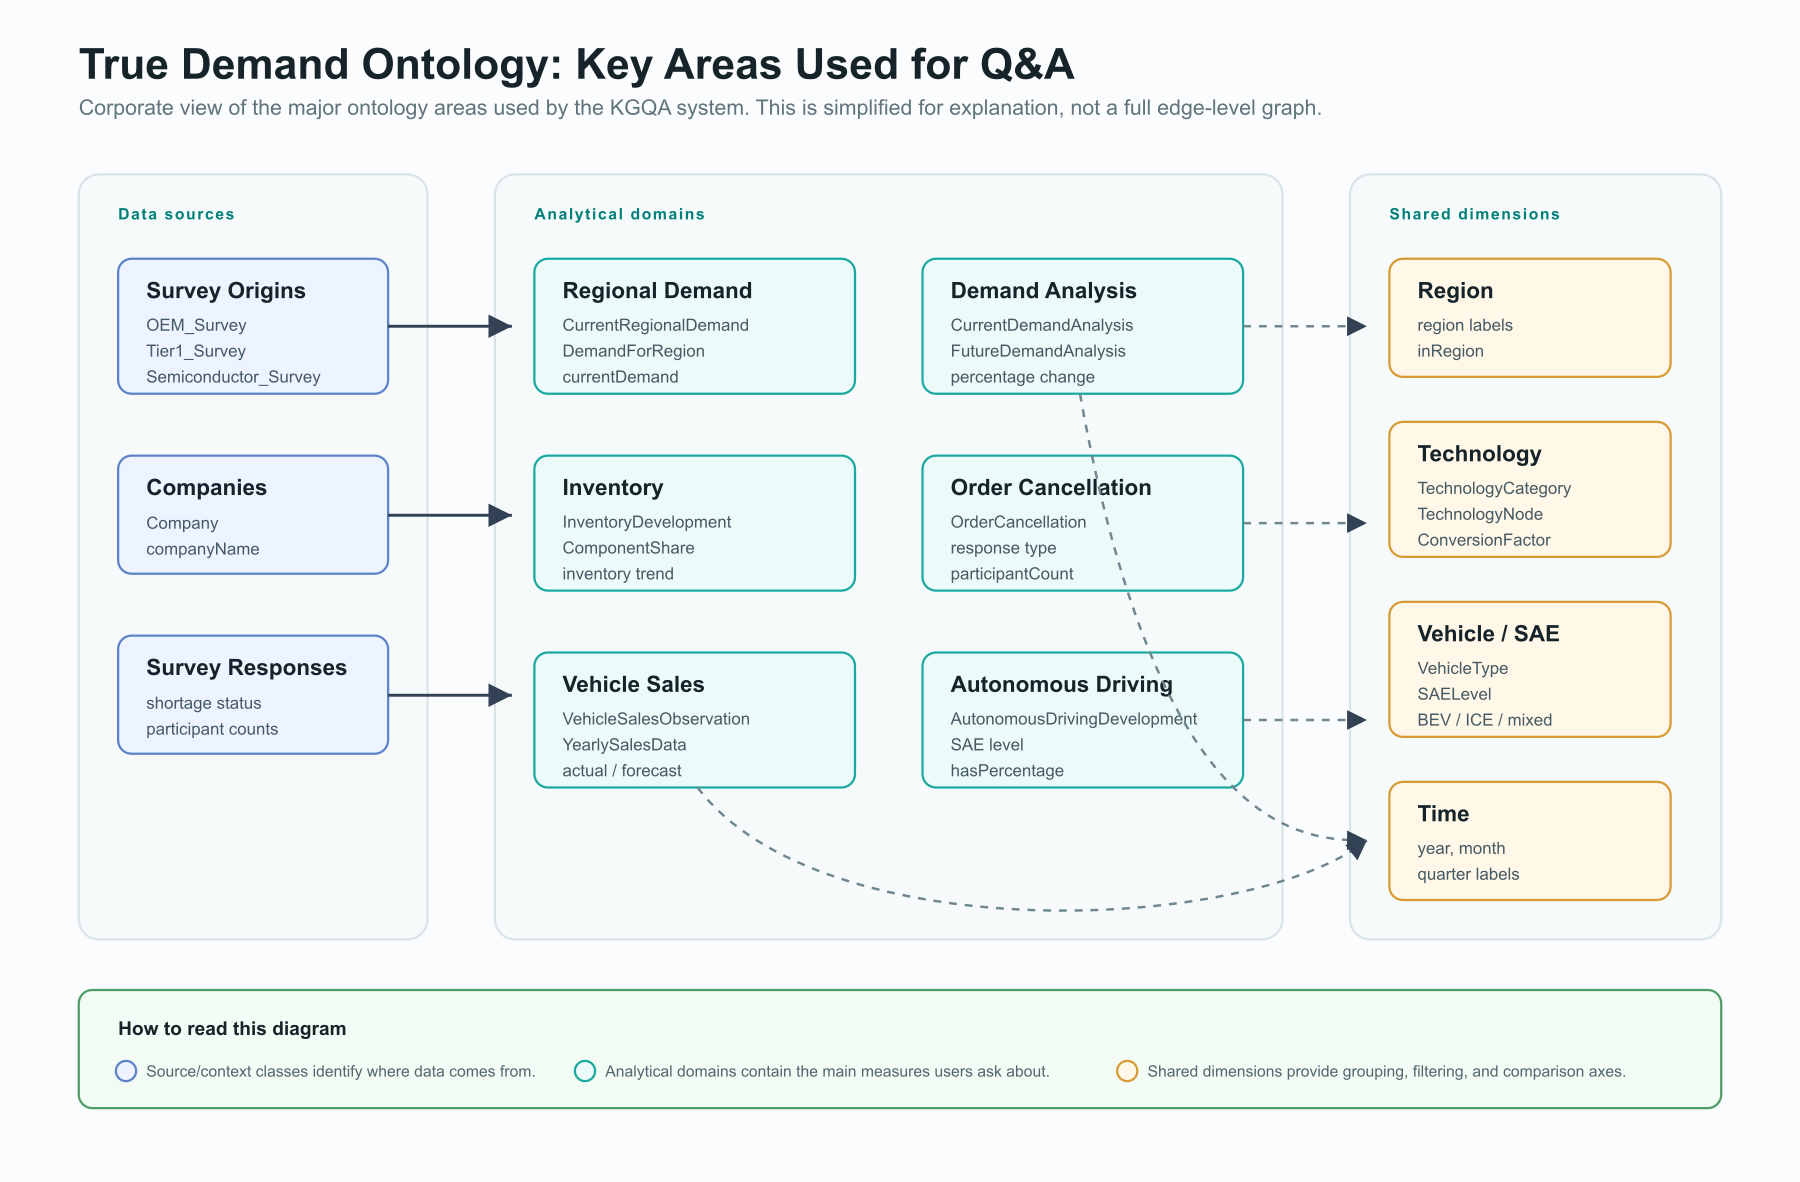
\includegraphics[width=0.95\textwidth]{true_demand_ontology_relationships.png}
\caption{Main ontology areas used by the True Demand KGQA system.}
\label{fig:true-demand-ontology-areas}
\end{figure}

\section{Ontology and Schema}
\label{sec:ontology-and-schema}

It is important to distinguish between the knowledge graph and the ontology/schema layer. The \textbf{knowledge graph} contains the actual RDF triples: concrete survey records, companies, regions, months, demand observations, vehicle-sales records, shortage indicators, and other instance-level data. The \textbf{ontology/schema} describes the conceptual structure of this graph: classes, properties, relationships, and expected connections between concepts.

The KGQA system uses both layers. SPARQL execution is performed over the full RDF graph. In contrast, candidate generation, validation, ranking, autocomplete, and direct routing use a schema abstraction derived from the graph. This schema abstraction is stored in \texttt{data/infineon/schema.json} and contains:

\begin{itemize}
    \item \textbf{Classes}, such as \texttt{Company}, \texttt{Region}, \texttt{FutureDemandAnalysis}, \texttt{CurrentDemandAnalysis}, \texttt{VehicleSalesObservation}, \texttt{OrderCancellation}, and \texttt{AutonomousDrivingDevelopment}.
    \item \textbf{Object-style predicates}, such as \texttt{hasSurveyOrigin}, \texttt{inRegion}, \texttt{forTimePeriod}, \texttt{analyzesVehicleType}, \texttt{analyzesTechnologyCategory}, \texttt{hasSAELevel}, and \texttt{forComponent}.
    \item \textbf{Data properties}, such as \texttt{totalDemand}, \texttt{percentageChange}, \texttt{totalDemandPercentageChange}, \texttt{unitsSold}, \texttt{participantCount}, \texttt{companyName}, \texttt{regionName}, and \texttt{periodLabel}.
    \item \textbf{Declared relationships}, which specify how classes are connected through predicates.
\end{itemize}

\begin{table}[htbp]
\centering
\caption{Distinction between schema, instance graph, and capability inventory.}
\label{tab:kg-schema-capability-layers}
\small
\begin{tabularx}{\textwidth}{
>{\raggedright\arraybackslash}p{3.2cm}
>{\raggedright\arraybackslash}p{5.2cm}
>{\raggedright\arraybackslash}X
}
\toprule
\textbf{Layer} & \textbf{Contains} & \textbf{Used for / example} \\
\midrule
Ontology / schema 
& Classes, predicates, relationships, and abstract graph structure. 
& Used for prompt construction, schema validation, visualization, and feature extraction. Example: \texttt{FutureDemandAnalysis}, \texttt{inRegion}. \\

Instance knowledge graph 
& Concrete survey records, observations, entities, and literal values. 
& Used for SPARQL execution, evidence retrieval, and answer generation. Example: a demand record with region and numeric value. \\

Capability inventory 
& Supported metric--dimension--aggregation combinations that return graph rows. 
& Used for direct routing, guided autocomplete, and clarification filtering. Example: future demand by region; vehicle sales by month. \\
\bottomrule
\end{tabularx}
\end{table}

The schema is used to constrain the LLM and reduce hallucinated query structures. For example, instead of asking the LLM to invent SPARQL over an unknown graph, the system provides canonical class and property names. This helps the model generate syntactically and structurally plausible candidates. However, schema validity is not sufficient for answer correctness. A query may use valid classes and predicates but still answer the wrong business question. For example, a question asking for a grouped regional breakdown may be incorrectly answered by a scalar count query, or a question about future demand may be confused with current demand if the candidate query selects the wrong analysis class.

For this reason, the schema is also used after candidate generation. The system extracts query-plan and answer-shape features from each candidate query, including:

\begin{itemize}
    \item whether the query uses aggregation such as \texttt{COUNT}, \texttt{SUM}, or \texttt{AVG};
    \item whether the query contains a \texttt{GROUP BY} clause when the question asks for a breakdown;
    \item whether the query selects the expected metric and dimension variables;
    \item whether the query uses the expected survey scope, such as OEM, Tier1, or Semiconductor;
    \item whether the query is a ranked query, a scalar query, a grouped table, or a list lookup.
\end{itemize}

This schema-derived representation is central to the selection problem studied in this thesis. The LLM often generates multiple valid-looking SPARQL queries. The system must then decide which candidate best matches the user intent. The ontology and schema therefore play two roles: they guide generation and provide features for downstream validation and ranking.

The extracted ontology file, \texttt{data/infineon/true\_demand\_ontology\_extracted.ttl}, is used primarily for schema inspection and explanation. It is smaller than the full graph because it contains the schema-level view rather than every instance-level survey record. During development, external ontology viewers were useful for checking the first schema-level representation, but the final user-facing system uses the integrated Streamlit graph overview and answer evidence graph instead. The full graph remains the execution backend for SPARQL queries.

\subsection{Digital Reference ontology integration}
\label{subsec:digital-reference-ontology}

In the final system version, the True Demand graph is complemented with a Digital Reference (DR) ontology resource. This addition was motivated by the requirement that users should not only ask analytical questions over survey data, but also ask questions about the model itself. Examples include ``What is True Demand?'', ``Define Future Demand'', ``What is a Technology Node?'', or ``What does \texttt{is processed by} mean?'' These questions are not ordinary data-aggregation questions. They ask for ontology-level descriptions, labels, and concept explanations.

The DR ontology is treated as a separate deterministic information source rather than as another LLM prompt. At startup, the system loads the DR ontology, extracts ontology terms, labels, comments, class/property types, and available definitions, and stores them in a lookup index. When the user asks a definition-style question, the router first attempts to resolve the requested term against this ontology index. If a unique ontology term is found, the answer can be produced without an LLM call. This is important for both reliability and cost: the definition answer should be grounded in the ontology, not invented by the LLM.

The combined system therefore uses two complementary graph layers:

\begin{itemize}
    \item \textbf{True Demand KG}: instance-level survey and analytical data used for SPARQL execution and numerical answers.
    \item \textbf{DR ontology}: conceptual and definitional information used for ontology-model questions and terminology explanation.
\end{itemize}

This distinction is important because the KG and the ontology answer different types of questions. The KG can answer questions such as ``Show current demand by region'' because it contains demand records and numeric values. The DR ontology can answer questions such as ``What is a Technology Node?'' because it contains concept-level definitions and model metadata. In the final interface, both are exposed through the same natural-language question box, but the routing layer decides whether the request is a KG analytics question, an ontology-definition question, an advisory question, or an unsupported question.

\begin{table}[htbp]
\centering
\caption{Question types covered by the final combined KG and DR ontology system.}
\label{tab:kg-dr-question-types}
\small
\begin{tabularx}{\textwidth}{
>{\raggedright\arraybackslash}p{3.8cm}
>{\raggedright\arraybackslash}p{5.0cm}
>{\raggedright\arraybackslash}X
}
\toprule
\textbf{Question type} & \textbf{Example} & \textbf{Primary route} \\
\midrule
KG analytical aggregation & ``Show total current demand from OEM customers by region.'' & True Demand KG, deterministic template or LLM-to-SPARQL fallback. \\
KG catalog lookup & ``Which technology categories are available?'' & True Demand KG catalog query. \\
Ontology definition & ``What is a Technology Node?'' & DR ontology deterministic definition lookup. \\
Ontology property explanation & ``What does \texttt{is processed by} mean?'' & DR ontology term/property lookup. \\
Advisory graph-grounded question & ``Based on current demand, which region should be monitored?'' & Deterministic advisory template over KG results. \\
\bottomrule
\end{tabularx}
\end{table}

For the thesis, it is useful to include a small schema example to show how a natural-language question maps to the graph. For example, a question about total current demand by region can be represented as a grouped SPARQL query over \texttt{DemandForRegion}, \texttt{Region}, \texttt{hasSurveyOrigin}, and \texttt{totalDemand}. Listing~\ref{lst:example-current-demand-query} shows a simplified query pattern.

\begin{lstlisting}[caption={Example graph-supported SPARQL query pattern for current demand by region.}, label={lst:example-current-demand-query}]
SELECT ?regionName (SUM(?demand) AS ?totalDemand) WHERE {
  ?entry a survey:DemandForRegion ;
         survey:hasSurveyOrigin ?origin ;
         survey:inRegion ?region ;
         survey:totalDemand ?demand .
  ?region survey:regionName ?regionName .
}
GROUP BY ?regionName
ORDER BY ?regionName
\end{lstlisting}

This example illustrates the structure that the QA system must recover from the user question: the metric is \texttt{totalDemand}, the analytical class is \texttt{DemandForRegion}, and the grouping dimension is \texttt{Region}. Similar patterns exist for future demand, shortage counts, vehicle sales, autonomous-driving indicators, inventory, and order-cancellation responses.

\section{Benchmark and Evaluation Data}
\label{sec:benchmark-evaluation-data}

In addition to the RDF graph itself, the thesis uses curated natural-language question sets and evaluation artefacts. These artefacts serve a different purpose from the graph. The graph defines what can be queried; the benchmark data defines how the KGQA system is evaluated. This separation is important because a question-answering benchmark must test not only whether the graph contains the relevant information, but also whether the system can identify the intended graph query from a natural-language request.

The repository contains an initial curated split of True Demand KGQA examples with training, development, and test files. These examples pair natural-language questions with expected query behavior and are used to develop prompts, schema features, ranking features, and evaluation scripts. The system also uses a larger set of generated and audited questions for system-level analysis, including efficiency and manual correctness evaluation. In the evaluation chapter, these datasets are used separately depending on the metric being reported.

\begin{table}[htbp]
\centering
\caption{Main data artefacts used for development and evaluation.}
\label{tab:evaluation-data-assets}
\footnotesize
\setlength{\tabcolsep}{4pt}
\begin{tabularx}{\textwidth}{
>{\raggedright\arraybackslash}p{2.9cm}
>{\raggedright\arraybackslash}p{2.0cm}
>{\raggedright\arraybackslash}X
}
\toprule
\textbf{Artefact} & \textbf{Size} & \textbf{Role} \\
\midrule
RDF graph & 1.16M triples & Full RDF execution backend for SPARQL queries
(\path{graph.ttl}) \\
Schema abstraction & 58 classes & Schema abstraction for prompting, validation, ranking, and routing
(\path{schema.json}) \\
DR ontology & DR ontology & Ontology definitions and model-level terminology lookup
(\path{DigitalReference.ttl}) \\
Ranker training data & 601 groups & Historical grouped candidate data for ML ranking
(\path{final1000_wf_train_ranker_data.json}) \\
KG selection benchmark & 1000 KG questions & Repaired LLM-only generation and selection benchmark
(\path{true_demand_final_1000_gold_repaired.json}) \\
Calibration split & 200 questions & Calibration split for guarded ML reranking
(\path{true_demand_final1000_calibration_200.json}) \\
Holdout split & 800 questions & Held-out selection evaluation after calibration
(\path{true_demand_final1000_holdout_800.json}) \\
Full-system benchmark & 1000 mixed questions & Final end-to-end system benchmark derived from the repaired KG benchmark, DR ontology questions, and advisory questions
(\path{true_demand_full_system_1000_repaired.json}) \\
DR ontology benchmark & 300 questions & Deterministic DR ontology definition benchmark
(\path{dr_ontology_benchmark_current.json}) \\
\bottomrule
\end{tabularx}
\end{table}

For the final evaluation, two types of results are reported separately. The first is \textbf{selection accuracy}, which evaluates how well the system selects the correct query among generated candidates. This is the scientific evaluation of ambiguity-aware query selection and is measured on candidate sets where LLM-generated alternatives exist. The second is \textbf{system accuracy}, which evaluates the end-to-end system, including deterministic direct templates, DR ontology definition routing, advisory templates, LLM-generated candidates, reranking, confidence routing, and answer synthesis. This distinction prevents direct graph-supported questions from artificially hiding the difficulty of the ambiguous selection problem, while still allowing the final system to be evaluated as an engineering artefact.

The final system benchmark contains 1000 mixed user-facing questions. Of these, 800 are KG analytics questions, 150 are DR ontology definition questions, and 50 are graph-grounded advisory questions. This composition reflects the intended user experience: a non-technical user may ask for numerical analysis, ask what a concept means, or ask for a data-grounded planning signal through the same interface.

The KG analytics part of the benchmark was repaired before the final evaluation. Early validation showed that some gold queries were syntactically valid but semantically wrong, while others returned empty results because they used unsupported paths or overly specific classes. These cases were inspected against the loaded RDF graph in Fuseki, corrected where the graph contained an appropriate answer path, and excluded from being treated as validated ground truth until they returned meaningful results. The final benchmark therefore reports results against the repaired gold dataset rather than against the first generated version of the question set.

\begin{table}[htbp]
\centering
\caption{Composition of the final 1000-question full-system benchmark.}
\label{tab:final-system-benchmark-composition}
\small
\begin{tabular}{lrr}
\toprule
\textbf{Question type} & \textbf{Questions} & \textbf{Share} \\
\midrule
True Demand KG analytics & 800 & 80.0\% \\
DR ontology definitions & 150 & 15.0\% \\
Graph-grounded advisory questions & 50 & 5.0\% \\
\midrule
Total & 1000 & 100.0\% \\
\bottomrule
\end{tabular}
\end{table}

\section{Data Limitations}
\label{sec:data-limitations}

The True Demand graph provides a valuable structured representation of survey-based semiconductor supply-chain information, but it also has limitations that directly affect KGQA performance. These limitations are important because they define what the system can answer reliably and what should be routed to clarification, fallback, or rejection.

\subsection{Survey-grounded coverage}

The graph is grounded in partner survey data and derived survey transformations. This means that the graph reflects what was collected, modeled, and transformed from the survey process. It does not contain every possible business fact about semiconductor supply chains. For example, the graph may contain future-demand percentages by region or technology category, but it may not contain every possible combination of product, customer, plant, lead time, or manufacturing process. A natural-language interface must therefore distinguish between questions that are answerable from the graph and questions that sound plausible but are not supported by the available data.

\subsection{Uneven class distribution}

The graph is highly uneven. Vehicle-sales observations dominate the instance-level graph, while several analytical areas contain much fewer records. This does not mean that the smaller areas are unimportant. Rather, they represent more aggregated survey outputs. However, this has practical consequences for query answering: some questions naturally return many rows, while others return only one or a few rows. The system therefore cannot rely only on schema terms. It must check whether a suggested query path actually returns data.

\subsection{Schema-valid does not mean semantically correct}

Many incorrect LLM-generated candidates are not syntactically invalid. They may use valid classes, valid predicates, and valid SPARQL syntax, but still answer a different question. For example:

\begin{itemize}
    \item a grouped breakdown may be replaced by a scalar count;
    \item a current-demand question may be answered using future-demand classes;
    \item a question asking for all groups may be answered by a ranked top-one query;
    \item a survey-specific question may omit the required survey origin;
    \item an answerable-looking query may return zero rows because the specific graph path does not exist.
\end{itemize}

This limitation is central to the thesis. It motivates the use of ML-based query selection, confidence routing, execution-aware validation, and graph-supported direct templates. The goal is not only to generate valid SPARQL, but to select a query that matches the intended business interpretation and returns graph-backed evidence.

\subsection{Ontology definitions and documentation coverage}

The True Demand graph contains class and relationship structure, but it does not always contain rich human-readable definitions for every class, metric, or business concept. For instance, a class such as \texttt{Company} may exist as a schema element, but the instance graph may not contain a detailed textual definition explaining what counts as a company in the business context. The final system mitigates this limitation by integrating the Digital Reference ontology as a deterministic definition source. However, the quality of definition answers remains bounded by the labels, comments, and metadata available in the ontology. If a concept is missing or poorly documented in the DR ontology, the system should not invent a definition; it should report that no reliable definition is available.

\subsection{Concrete examples of graph constraints}
\label{subsec:concrete-graph-constraints}

Several limitations only become visible when natural-language questions are executed against the graph. These examples are useful because they show why the system cannot rely only on the ontology labels:

\begin{itemize}
    \item \textbf{Time granularity is domain-specific.} Vehicle-sales observations support month-level questions, but future-demand and current-demand survey outputs are not necessarily available at the same monthly granularity. Therefore, ``vehicle sales by month'' can be graph-supported while ``future demand by month'' may not be.
    \item \textbf{Survey scope changes the meaning of a query.} Demand, shortage, inventory, and autonomous-driving records may be associated with different survey origins such as OEM, Tier1, or Semiconductor. Omitting this scope can lead to a broader or different interpretation than the user intended.
    \item \textbf{Breakdown and ranking are different answer shapes.} A question phrased as ``by region'' or ``by vehicle type'' normally asks for a grouped table. It should not be automatically converted into ``which region is highest'' unless the user explicitly asks for a top, maximum, or highest value.
    \item \textbf{Catalog entities do not guarantee analytical support.} A region, technology category, or vehicle type may exist in the graph catalog, but not every metric is connected to every catalog value through a non-empty analytical path.
    \item \textbf{Counts can be misleading if the user asks for a metric.} A count of records may be valid SPARQL, but it is not the same as a total demand value, average percentage, or grouped business metric.
\end{itemize}

These examples motivated the final design of answerable autocomplete and capability-guided direct templates. The guiding principle is that user-facing suggestions should represent answerable graph paths, not merely possible ontology terms.

\subsection{Implications for the KGQA system}

These data limitations shaped several design decisions in the final system:

\begin{itemize}
    \item \textbf{Graph-supported autocomplete and guided examples}: suggested terms and generated questions should be backed by query paths that return rows.
    \item \textbf{Direct deterministic templates}: frequent graph-supported question patterns can be answered without calling the LLM.
    \item \textbf{Execution-aware selection}: candidate queries that return no rows or violate the requested answer shape should be penalized or avoided.
    \item \textbf{Clarification}: when multiple plausible interpretations remain, the system should ask the user to choose rather than force an unreliable answer.
    \item \textbf{Separation of metrics}: selection accuracy, system accuracy, coverage, and LLM cost must be reported separately because direct graph-supported questions and LLM-needed ambiguous questions have different difficulty levels.
\end{itemize}

Table~\ref{tab:data-limitations} summarizes the main limitations and their system-level consequences.

\begin{table}[htbp]
\centering
\caption{Data limitations and their implications for the KGQA system.}
\label{tab:data-limitations}
\small
\begin{tabularx}{\textwidth}{
>{\raggedright\arraybackslash}p{3.8cm}
>{\raggedright\arraybackslash}p{5.2cm}
>{\raggedright\arraybackslash}X
}
\toprule
\textbf{Limitation} & \textbf{Effect} & \textbf{System response} \\
\midrule
Survey-grounded coverage & Not every business question is answerable from the graph. & Capability inventory and graph-supported suggestions. \\
Uneven class distribution & Some domains return many rows, others only few. & Execution checks and row-aware guidance. \\
Schema-valid but semantically wrong candidates & Valid SPARQL can still answer the wrong question. & ML reranking and answer-shape features. \\
Missing combinations of dimensions & Some plausible breakdowns return zero rows. & Direct templates only for supported paths. \\
Incomplete ontology documentation & Definition questions are only as complete as available DR labels and comments. & Deterministic DR lookup with no-invention fallback. \\
\bottomrule
\end{tabularx}
\end{table}

Overall, the True Demand graph provides a realistic and challenging foundation for LLM-based KGQA. It is large enough to require structured querying, rich enough to support multiple analytical domains, and complex enough to expose ambiguity in query selection. At the same time, its survey-grounded and uneven nature makes it necessary to combine LLM generation with deterministic graph validation, ML-based selection, and user-facing clarification.




% Revised Chapter 4: System Architecture
% Suggested LaTeX packages in the thesis preamble:
% \usepackage{graphicx}
% \usepackage{float}
% \usepackage{booktabs}
% \usepackage{tabularx}
% \usepackage{array}
% \usepackage{subcaption}
% \usepackage{listings}

\chapter{System Architecture}
\label{chap:system-architecture}

This chapter describes the architecture of the True Demand KGQA system. The system is designed as a controlled natural-language interface over a survey-grounded semiconductor supply-chain knowledge graph. The central architectural challenge is not only to generate SPARQL from a user question, but to decide whether a generated interpretation is graph-supported, semantically aligned with the user's intent, executable, and safe to present as an automatic answer.

The system therefore follows a hybrid architecture. Deterministic graph-supported routing is used for frequent, unambiguous analytical questions. The LLM is used when a question requires flexible interpretation and candidate generation. Generated candidates are not executed directly; they are validated, featurized, ranked, and routed through a confidence policy. When the system cannot select one interpretation reliably, the user is asked to choose between natural-language clarification options. This design separates candidate generation from candidate selection and makes the overall system more reliable than a naive single-step LLM-to-SPARQL pipeline.

The main design principle is that the LLM is one component inside a broader decision pipeline, not the final authority of the system. This is necessary for three reasons. First, a syntactically valid SPARQL query can still answer the wrong business question if it uses the wrong analytical class, aggregation, grouping dimension, or survey scope. Second, LLM calls are costly and unnecessary for many graph-supported questions whose SPARQL structure is already known. Third, a business user should not be forced to inspect raw SPARQL when a question is ambiguous; the system should instead present understandable alternatives such as ``average future demand by region'' or ``count companies by shortage status''.

Figure~\ref{fig:system-architecture-pipeline} gives the high-level view of the final system. The user accesses the Streamlit application through a web browser. The application performs request routing and capability resolution before deciding whether the question can be answered through a deterministic graph template or whether it must enter the LLM-based candidate-generation and ranking path. The selected query is executed against the True Demand graph through the SPARQL runtime, and the answer is synthesized into a user-facing explanation with optional evidence graph and technical details.

\section{Architectural Requirements}
\label{sec:architectural-requirements}

\begin{figure}[htbp]
    \centering
    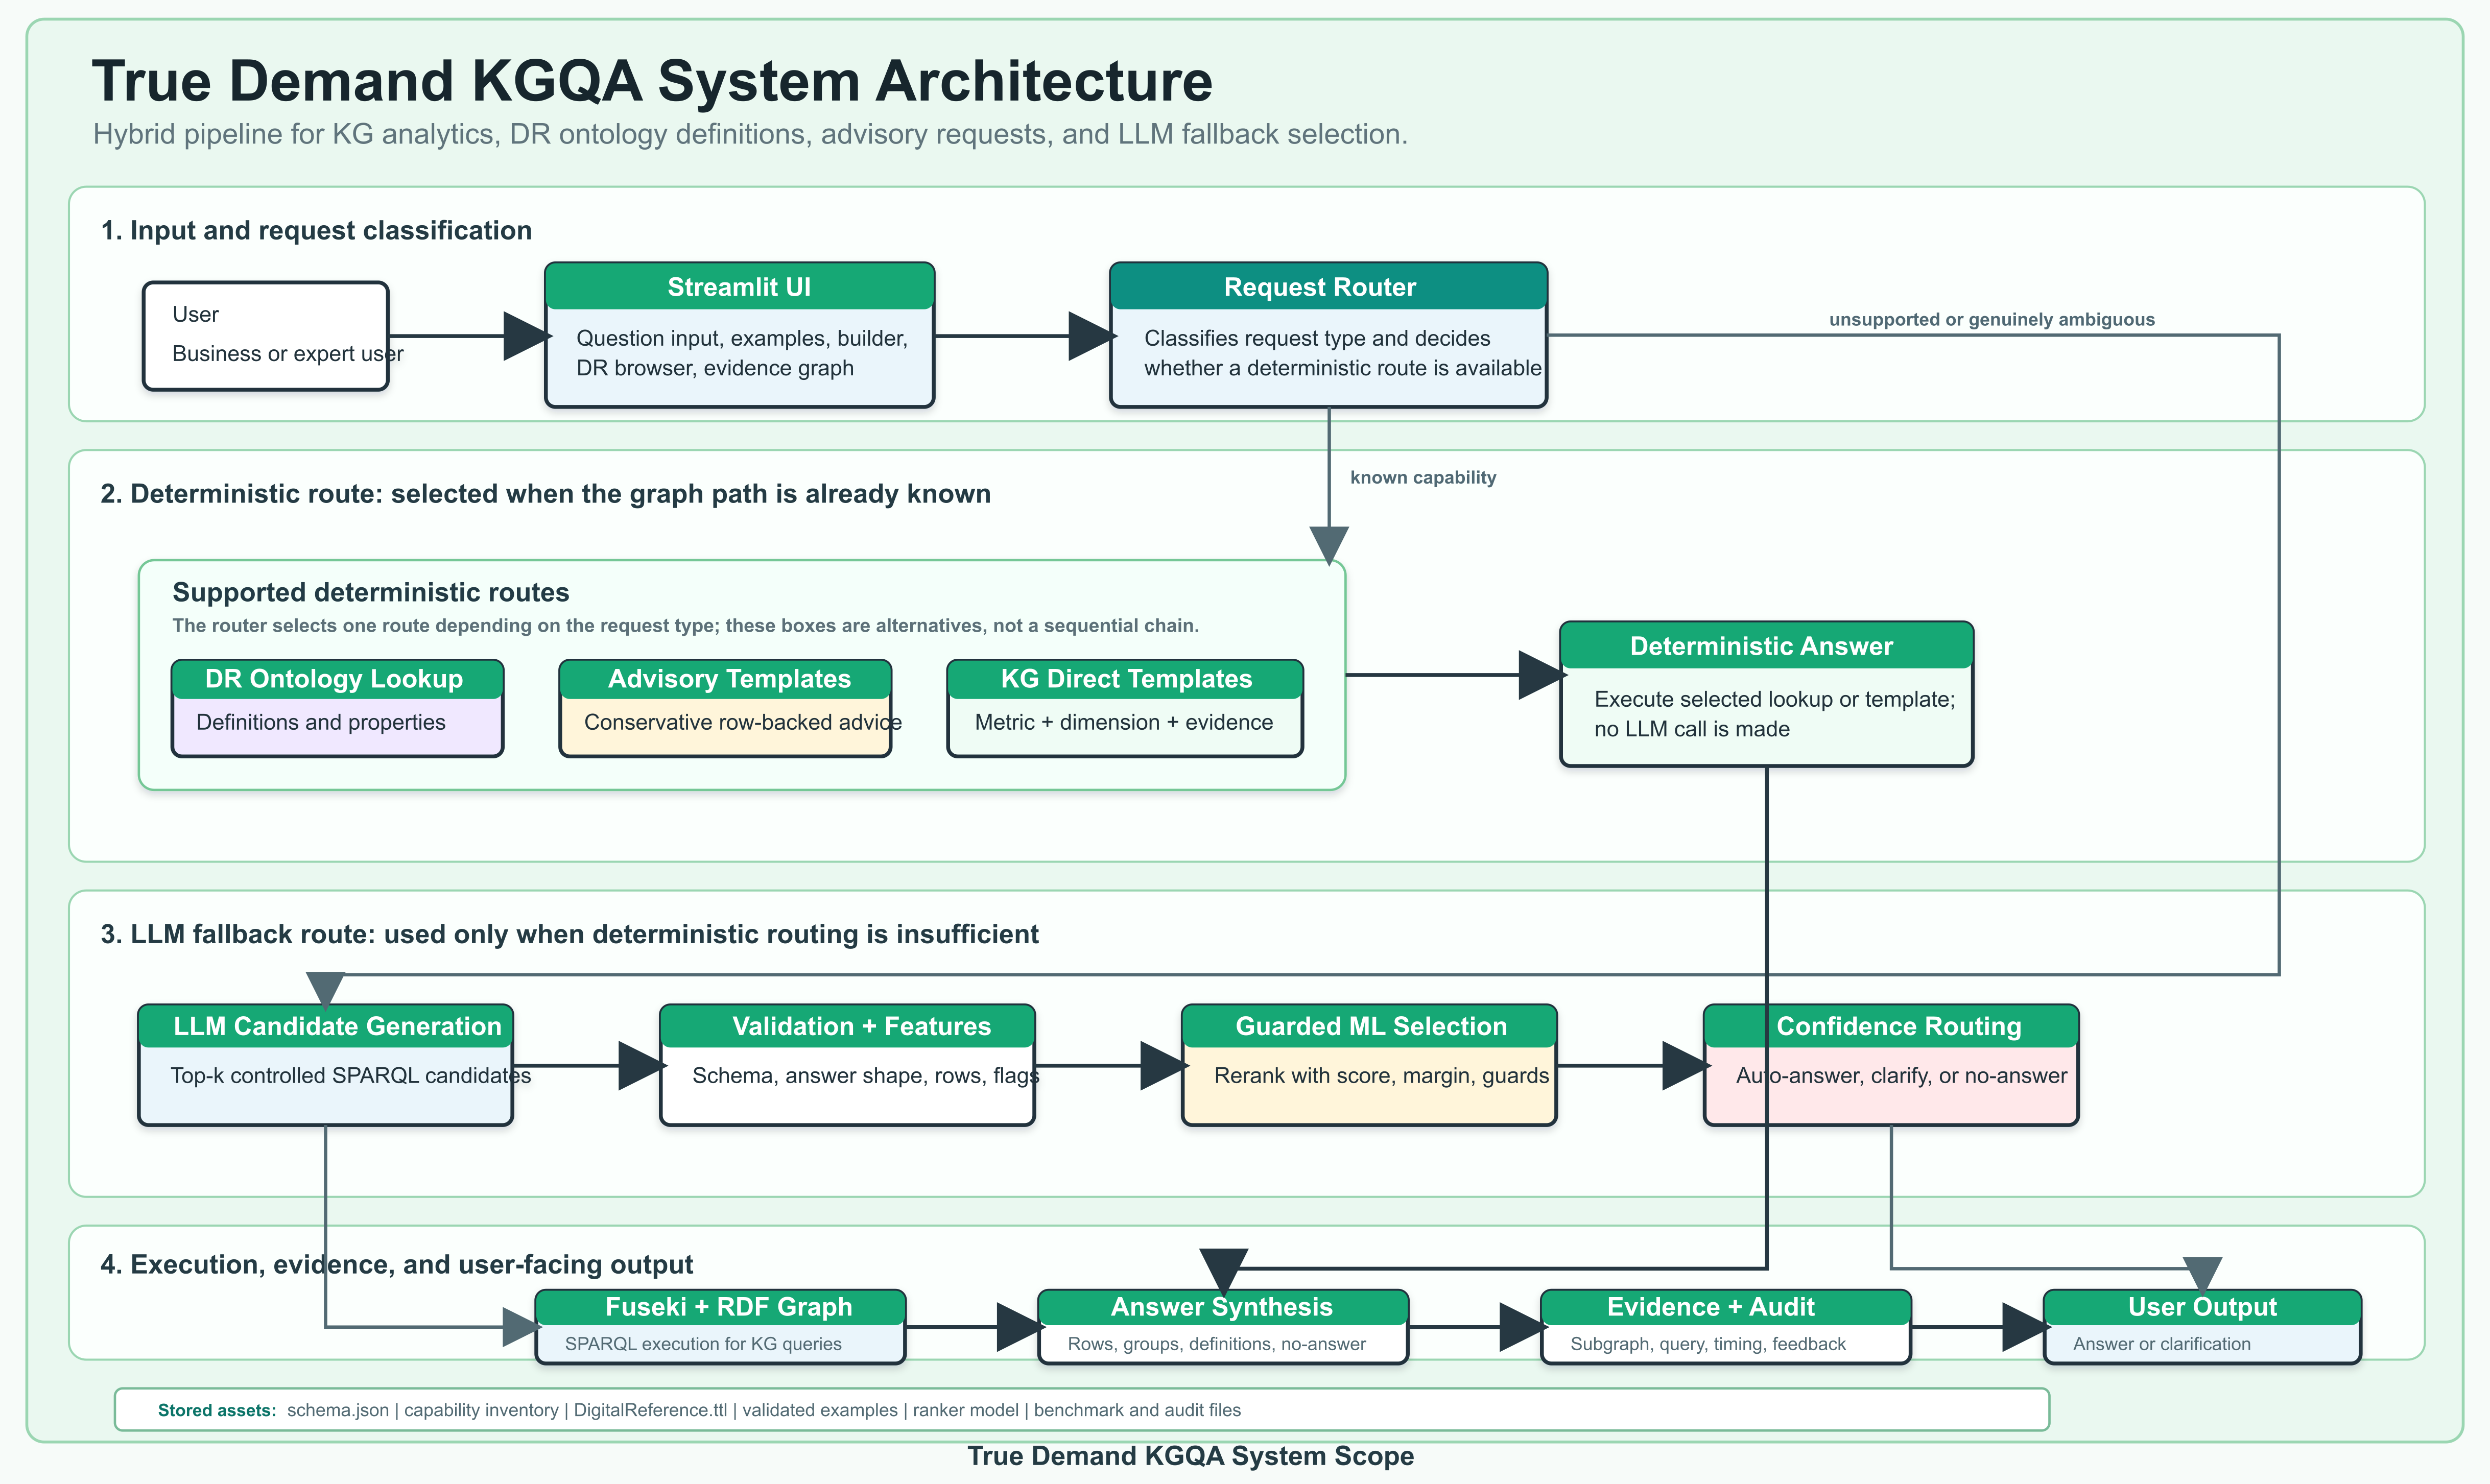
\includegraphics[width=0.95\textwidth]{system_architecture_pipeline.png}
    \caption{Overall architecture of the True Demand KGQA system. The LLM generates candidate interpretations only when deterministic graph-supported routing is insufficient; downstream validation, ranking, confidence routing, and execution determine whether an answer is returned automatically or whether clarification is required.}
    \label{fig:system-architecture-pipeline}
\end{figure}

The architecture was derived from the practical requirements of enterprise KGQA over the True Demand graph. The system must support natural-language access for users who do not know SPARQL, but it must also avoid presenting unsupported or semantically wrong graph results. Table~\ref{tab:architecture-requirements} summarizes the main requirements and the architectural mechanism used to address each one.



\begin{table}[htbp]
\centering
\caption{Architectural requirements and corresponding system mechanisms.}
\label{tab:architecture-requirements}
\small
\begin{tabularx}{\textwidth}{
>{\raggedright\arraybackslash}p{3.0cm}
>{\raggedright\arraybackslash}p{5.0cm}
>{\raggedright\arraybackslash}X
}
\toprule
\textbf{Requirement} & \textbf{Problem addressed} & \textbf{Architectural mechanism} \\
\midrule
Natural-language access & Business users should not need to know SPARQL or ontology identifiers. & Streamlit question interface, guided examples, autocomplete, answer synthesis. \\
Graph grounding & Answers must be supported by the RDF graph rather than generated from free text. & SPARQL execution over Fuseki/RDFLib, row previews, evidence graph. \\
Semantic correctness & Valid SPARQL can still use the wrong metric, class, dimension, or answer shape. & Schema validation, query-plan features, answer-contract features, ML reranking. \\
Cost control & LLM calls should not be used for simple known graph patterns. & Direct graph-supported routing and capability inventory. \\
Ambiguity handling & Some questions have multiple plausible interpretations. & Candidate-set scoring, score margin, entropy, safety flags, clarification UI. \\
Auditability & The system should expose why an answer or clarification was produced. & Technical SPARQL expander, developer diagnostics, routing metadata, execution logs. \\
\bottomrule
\end{tabularx}
\end{table}

These requirements motivate a staged architecture. Each stage either narrows the interpretation space, validates the candidate query, or decides whether automatic answering is safe. This is different from a direct LLM-to-SPARQL design, where a single generated query is immediately executed and the user may receive a confident but wrong answer.

\section{Runtime Component View}
\label{sec:runtime-component-view}

At runtime, the system consists of five main component groups: the Streamlit user interface, the routing and capability layer, the LLM candidate-generation layer, the validation/ranking layer, and the execution/answer-synthesis layer. Stored assets such as the schema abstraction, ranking model, benchmark files, capability inventory, and audit reports support these runtime components.


\begin{table}[htbp]
\centering
\caption{Main runtime components of the system architecture.}
\label{tab:runtime-components}
\small
\begin{tabularx}{\textwidth}{
>{\raggedright\arraybackslash}p{3.1cm}
>{\raggedright\arraybackslash}p{5.5cm}
>{\raggedright\arraybackslash}X
}
\toprule
\textbf{Component} & \textbf{Responsibility} & \textbf{Main artefacts or outputs} \\
\midrule
Streamlit application & Provides the user-facing interface for questions, suggestions, answers, clarification cards, evidence, feedback, and developer settings. & User question, selected clarification option, answer panel, evidence graph, diagnostic views. \\
Request and capability routing & Determines whether the request is a graph question, definition request, unsupported request, or directly answerable graph-supported capability. & Route label, capability report, optional deterministic SPARQL template. \\
LLM candidate generation & Produces multiple SPARQL candidates when deterministic routing is insufficient. & Candidate SPARQL queries with source metadata. \\
Validation and feature extraction & Checks syntax, schema consistency, semantic coverage, answer shape, grouping, aggregation, scope, and execution behavior. & Candidate feature vectors, safety flags, row counts, query-shape metadata. \\
ML and confidence selection & Scores candidate queries, applies guarded reranking, and decides whether to answer, clarify, or avoid a forced answer. & Selected candidate, confidence decision, clarification alternatives. \\
Execution and answer synthesis & Executes the selected SPARQL query and converts result rows into a readable answer. & Graph rows, synthesized answer, evidence graph, technical SPARQL. \\
Stored assets & Provide schema, examples, trained models, capability definitions, benchmark data, and logs. & \texttt{schema.json}, ranking model, capability inventory, audit CSV, benchmark files. \\
\bottomrule
\end{tabularx}
\end{table}

The component view is important because it makes clear that the LLM does not directly control the answer. It generates possible graph interpretations. The rest of the system decides whether any of these interpretations are valid, graph-supported, and reliable enough for the user.

\section{Overall Pipeline}
\label{sec:overall-pipeline}

The full runtime pipeline is shown in Figure~\ref{fig:runtime-flow}. The process begins when the user submits a natural-language question. The system first performs lightweight routing and capability resolution. If the question matches exactly one supported capability and the required dimensions and aggregation are clear, the system uses a deterministic SPARQL template. If the question is not directly resolvable, the LLM generates a set of candidate SPARQL queries. These candidates are validated, featurized, ranked, and checked by the confidence router. Only after this selection process is a query executed and synthesized into an answer.

For interactive use, the implementation also includes runtime safety controls that are stricter than the offline evaluation scripts. User-facing requests are handled under a short interactive time budget, configured around 10 seconds for deployment testing. Deterministic routes and validated graph templates are attempted first because they avoid LLM latency. If the request requires LLM fallback and the generation or ranking path does not complete within the budget, the interface stops waiting for an automatic answer and returns supported clarification options instead of leaving the user in an indefinite loading state.

The timeout guard is not treated as evidence that the question is unanswerable. It is a user-experience and safety mechanism: the system may still be able to answer the request offline or with a more precise formulation, but the interactive interface prefers a bounded response with explicit alternatives. The same guard is used for broad demand questions, unsupported relative-time windows such as ``the past three months'', and ambiguous requests where the graph contains related but not identical time granularities.

\begin{figure}[htbp]
    \centering
    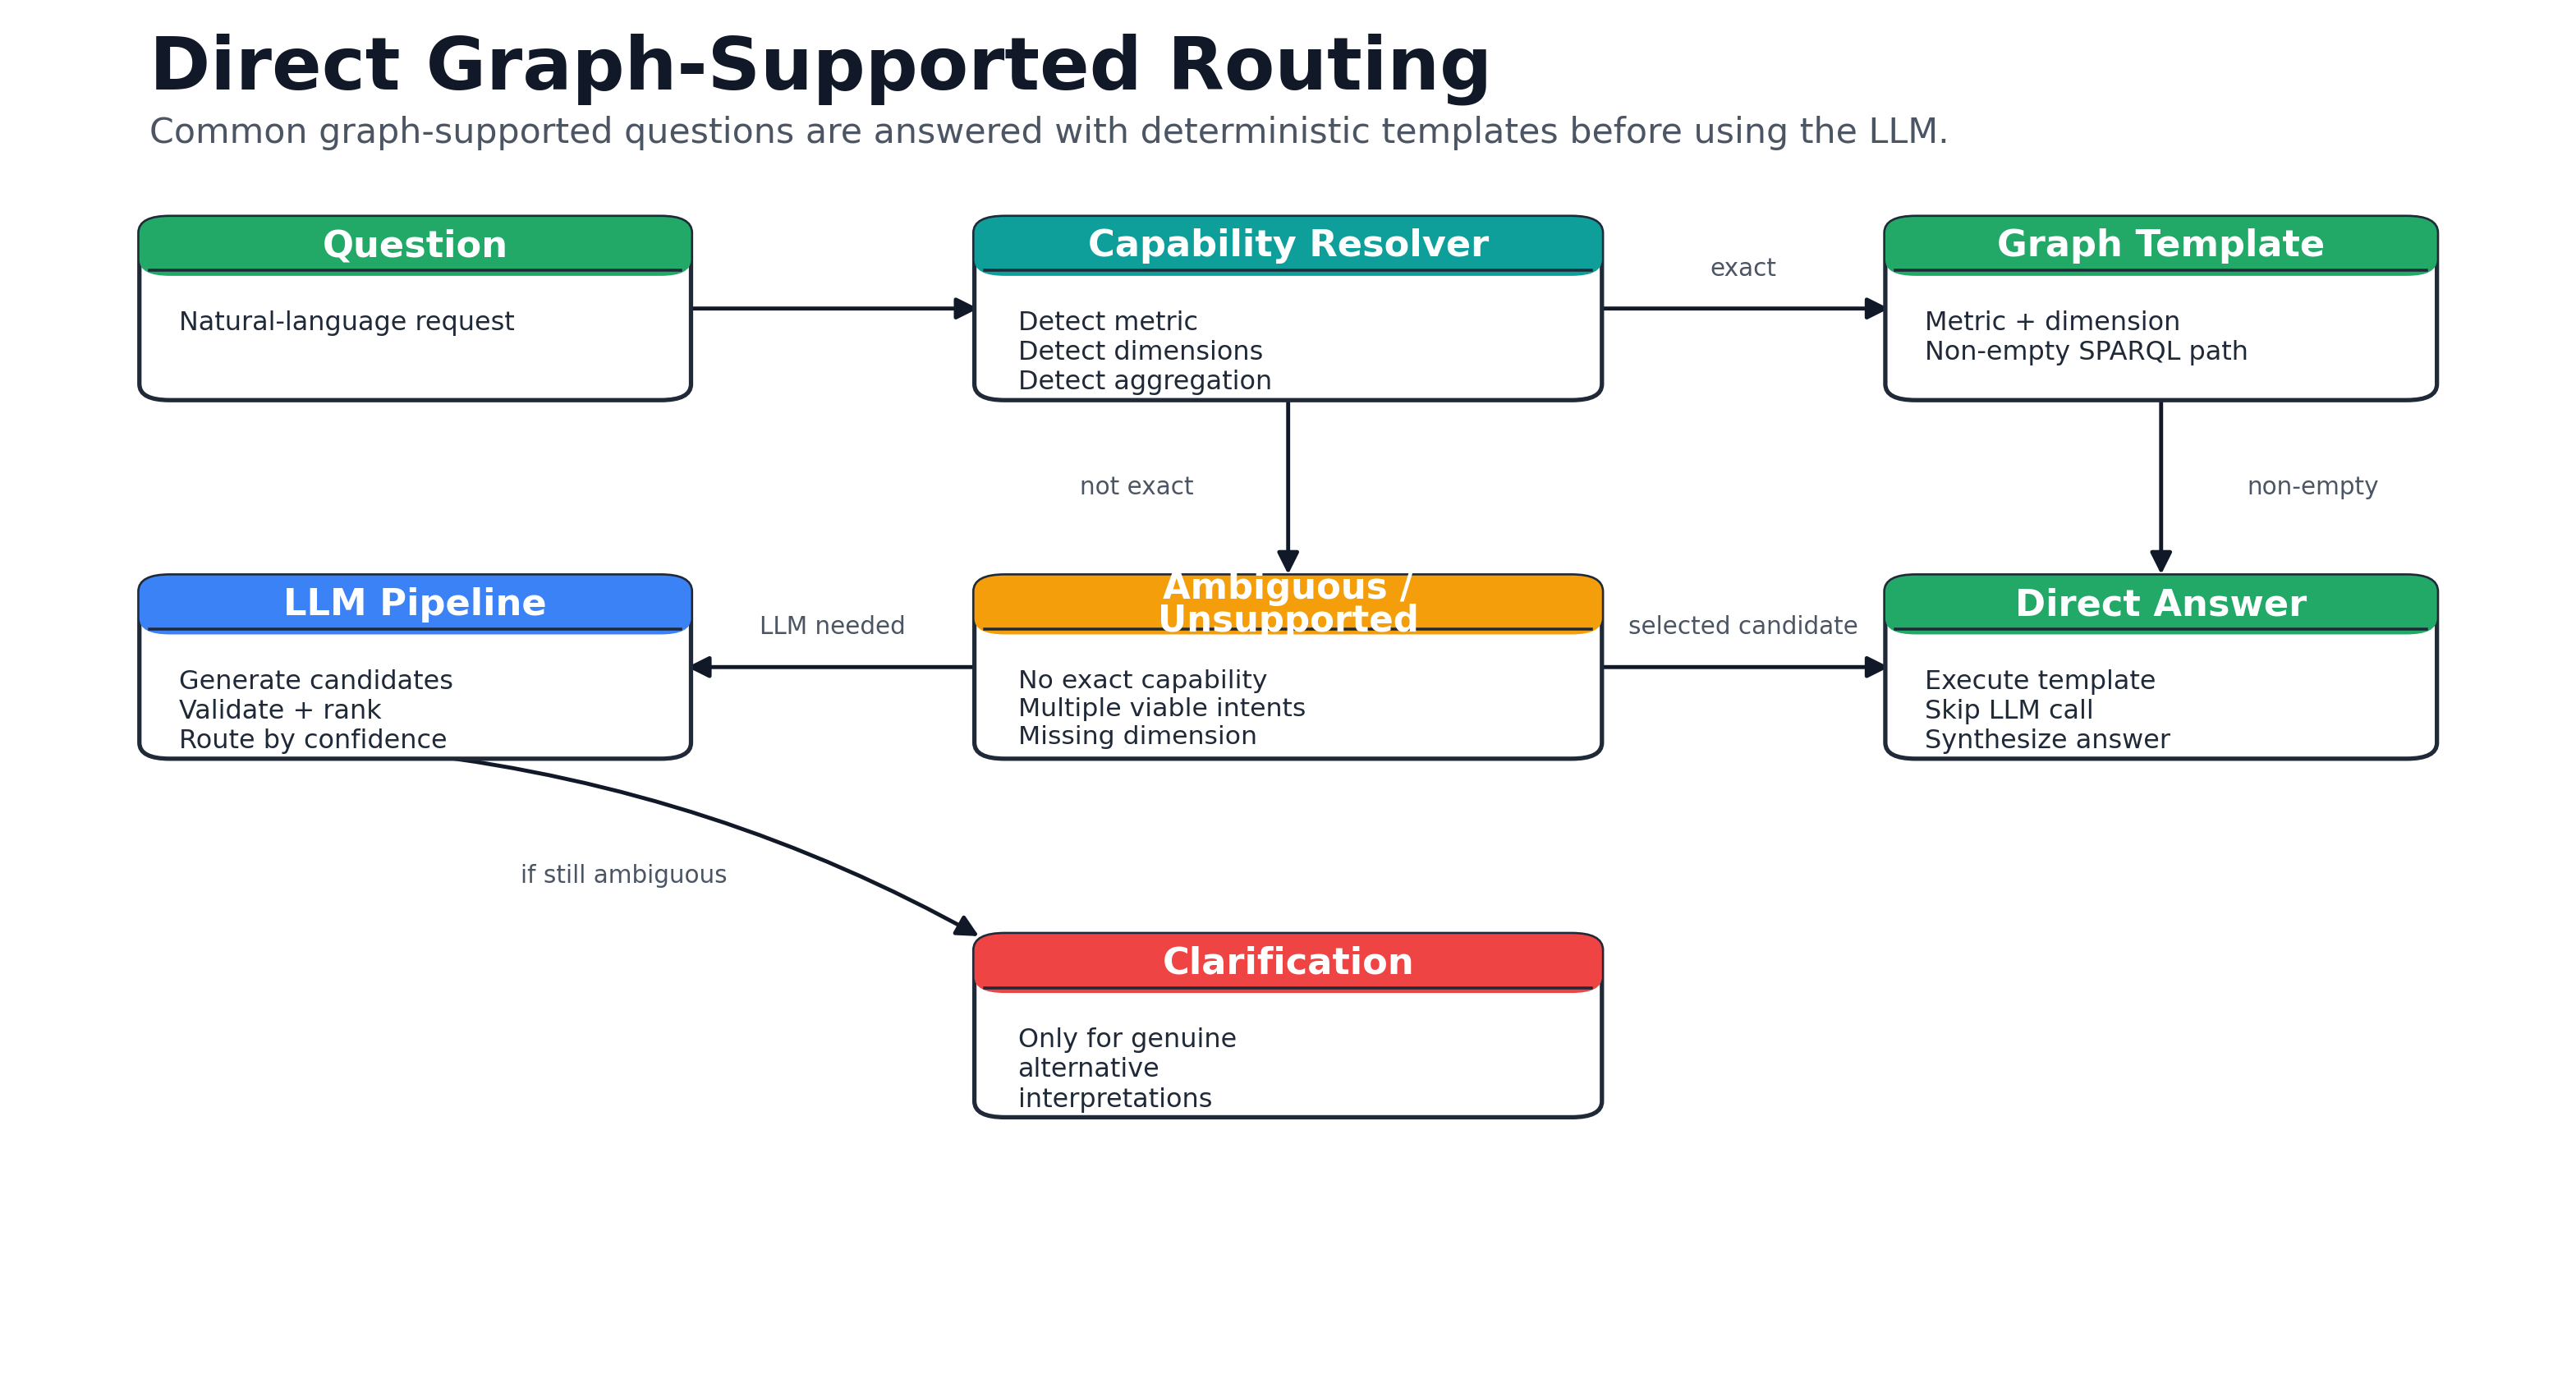
\includegraphics[width=\textwidth]{direct_graph_supported_routing.png}
    \caption{Direct graph-supported routing before LLM candidate generation. The system first attempts to resolve a question through the capability inventory. If exactly one supported graph path matches, the query is executed deterministically; otherwise the request is passed to the LLM/ranking path or clarification.}
    \label{fig:runtime-flow}
\end{figure}

\begin{table}[htbp]
\centering
\caption{Runtime stages in the True Demand KGQA pipeline.}
\label{tab:runtime-stages}
\small
\begin{tabularx}{\textwidth}{
>{\raggedright\arraybackslash}p{3.2cm}
>{\raggedright\arraybackslash}p{5.2cm}
>{\raggedright\arraybackslash}X
}
\toprule
\textbf{Stage} & \textbf{Purpose} & \textbf{Output} \\
\midrule
Question intake & Collect the user's natural-language request. & Raw question and UI metadata. \\
Request routing & Decide whether the request is a KG question, definition question, unsupported question, or graph-supported analytical query. & Route label. \\
Capability resolution & Match the question to supported metric--dimension--aggregation combinations. & Capability report and optional template. \\
Candidate generation & Generate multiple SPARQL candidates when no deterministic route is safe. & Candidate set. \\
Validation and feature extraction & Convert each query into structured validity, schema, semantic, shape, and execution features. & Candidate feature table. \\
Selection and confidence routing & Rank candidates and decide between automatic answer, clarification, or no forced answer. & Selected candidate or clarification options. \\
Execution & Execute the selected query against the True Demand graph. & Rows, errors, row count, evidence paths. \\
Answer synthesis & Produce a readable answer consistent with the requested answer shape. & User-facing answer and optional evidence graph. \\
\bottomrule
\end{tabularx}
\end{table}

\begin{lstlisting}[
caption={Simplified runtime pipeline for one user question.},
label={lst:overall-runtime-pipeline},
breaklines=true,
basicstyle=\ttfamily\small
]
question = read_user_question()

route = route_request(question)
if route is not graph_question:
    return route_specific_response(route)

capability = resolve_graph_capability(question)
if capability.has_exact_supported_template():
    query = capability.direct_query
    rows = execute(query)
    return synthesize_answer(question, query, rows)

candidates = generate_llm_candidates(question, schema_context)
features = extract_validation_features(candidates, question)
ranked = rank_candidates(features)
decision = confidence_route(ranked)

if decision == auto_answer:
    rows = execute(ranked.top.query)
    return synthesize_answer(question, ranked.top.query, rows)

if decision == clarify:
    return show_clarification_choices(ranked.top_k)

return controlled_no_answer()
\end{lstlisting}

The key architectural idea is the separation of \emph{generation} and \emph{selection}. The LLM proposes candidate interpretations, but the system validates and selects them using graph-aware mechanisms. This is the core contribution of the architecture.

\section{Direct Graph-Supported Routing}
\label{sec:direct-graph-supported-routing}

Direct graph-supported routing is the first major control layer. Its purpose is to answer frequent and unambiguous graph questions without invoking the LLM. A direct route is not a simple keyword shortcut. It is a capability-level match: the system must identify the intended metric, the grouping dimension, the aggregation type, and a valid SPARQL path that is known to return graph rows.

For example, a question such as ``show sales volume by month'' can be mapped directly to a vehicle-sales template because the metric, time dimension, and aggregation pattern are supported. Similarly, current demand by region, shortage counts by survey group, and autonomous-driving averages by vehicle type can be answered by deterministic templates when the user's request is specific enough. In contrast, a vague question such as ``demand by region'' should not automatically be converted into one template if both current demand and future demand remain plausible.

\begin{table}[htbp]
\centering
\caption{Examples of direct graph-supported route families.}
\label{tab:direct-route-families}
\small
\begin{tabularx}{\textwidth}{
>{\raggedright\arraybackslash}p{3.2cm}
>{\raggedright\arraybackslash}p{5.0cm}
>{\raggedright\arraybackslash}X
}
\toprule
\textbf{Family} & \textbf{Direct patterns} & \textbf{Reason for direct routing} \\
\midrule
Current/regional demand & Total or average demand by region, survey group, or vehicle type. & Metric and grouping dimensions are explicit and graph-supported. \\
Future demand & Future-demand change by region, quarter, vehicle type, or technology category. & Predefined analytical paths exist for supported dimensions. \\
Vehicle sales & Vehicle-sales units by month, year, or vehicle type. & Stable observation table and time dimensions are available. \\
Shortage & Count companies by shortage status or survey group. & Count shape and target class are clear. \\
Autonomous driving & Average development percentage by vehicle type, SAE level, year, or survey group. & AVG answer shape and grouping dimensions are known. \\
Inventory & Inventory development by component, technology category, or trend. & Supported survey-derived inventory classes exist. \\
Order cancellation & Cancellation responses by technology category or response type. & Count/SUM patterns are stable. \\
\bottomrule
\end{tabularx}
\end{table}

\begin{lstlisting}[
caption={Conservative direct-routing policy.},
label={lst:direct-routing-policy},
breaklines=true,
basicstyle=\ttfamily\small
]
report = capability_registry.resolve(question)

if report.primary_capability is None:
    continue_to_llm_pipeline()

if report.has_one_capability():
    if report.has_one_requested_dimension():
        query = capability_registry.direct_query_for(report)

        if query exists and query_returns_rows(query):
            return direct_answer(query)

continue_to_llm_pipeline_or_clarification()
\end{lstlisting}

The direct-routing layer is intentionally conservative. It should answer directly only when the graph path is known and the user's intent is specific enough. This avoids a common failure mode of natural-language interfaces: making a broad user question look more precise than it actually is.

The final repaired 1000-question audit supports this design choice. In that run, 514 questions were handled through deterministic graph-supported or ontology-supported routing, while 486 entered the LLM fallback route. This corresponds to 51.4\% deterministic coverage and 48.6\% LLM fallback coverage. Table~\ref{tab:architecture-audit-snapshot} summarizes the main architecture-level audit signals. These values are reported in more detail in the evaluation chapter, but they are useful here to justify the architectural separation between deterministic routing and candidate-based ranking.

\begin{table}[htbp]
\centering
\caption{Architecture-level snapshot from the final 1000-question audit file.}
\label{tab:architecture-audit-snapshot}
\small
\begin{tabularx}{\textwidth}{
>{\raggedright\arraybackslash}p{6cm}
>{\raggedright\arraybackslash}X
}
\toprule
\textbf{Metric} & \textbf{Observed value in audit file} \\
\midrule
Evaluated questions & 1000 \\
Deterministic / graph-supported route & 514 questions (51.4\%) \\
LLM fallback route & 486 questions (48.6\%) \\
DR ontology definition route & 150 questions (15.0\%) \\
Advisory route & 50 questions (5.0\%) \\
Validated-retrieval selected source & 330 questions \\
Capability-inventory selected source & 326 questions \\
Infineon LLM selected source & 150 questions \\
Observed cold-cache LLM calls & 486 calls \\
Estimated cold-cache LLM-call reduction & 51.4\% \\
\bottomrule
\end{tabularx}
\end{table}


\section{LLM Candidate Generation}
\label{sec:llm-candidate-generation}

The LLM is used when deterministic graph-supported routing is insufficient. In this architecture, the LLM does not generate the final answer directly. Its role is to generate candidate SPARQL queries that represent plausible interpretations of the user's question. The candidate set is then inspected by the downstream validation and ranking components.

The candidate-generation prompt contains the user question, schema context, graph naming conventions, examples of valid SPARQL structures, and capability hints where available. The schema context restricts the model to known classes and predicates, while the capability hints encourage graph-supported analytical patterns. In the final candidate-generation benchmark, each unresolved question requested up to eight SPARQL candidates at temperature 0.2. Candidate sets may contain fewer than eight usable candidates after duplicate removal, syntax validation, and limited repair of invalid candidates. In some cases, a family-aware schema slice can be used to reduce prompt size by focusing on the most relevant graph area. If routing confidence is low, the system can use a broader schema context to avoid excluding the correct family too early.

\begin{lstlisting}[
caption={Abbreviated LLM candidate-generation prompt structure.},
label={lst:candidate-generation-prompt},
breaklines=true,
basicstyle=\ttfamily\small
]
Task: Generate up to K candidate SPARQL SELECT queries for the True Demand KG.
Question: {user_question}

Use only the provided schema vocabulary and namespace conventions.
Prefer graph-supported analytical patterns from the capability hints.
Do not invent classes, predicates, or literal values that are not present.
Return multiple plausible interpretations when the question is ambiguous.

Schema slice: {classes, predicates, relationships, datatype properties}
Capability hints: {known metric-dimension-aggregation patterns}
Validated examples: {few-shot question-query pairs}

Output: JSON list of candidates with SPARQL query and short rationale.
\end{lstlisting}

\begin{table}[htbp]
\centering
\caption{Inputs used during LLM candidate generation.}
\label{tab:candidate-generation-inputs}
\small
\begin{tabularx}{\textwidth}{
>{\raggedright\arraybackslash}p{3.0cm}
>{\raggedright\arraybackslash}p{5.3cm}
>{\raggedright\arraybackslash}X
}
\toprule
\textbf{Input} & \textbf{Description} & \textbf{Purpose} \\
\midrule
User question & Natural-language request entered in the UI. & Provides the intended metric, dimension, scope, and answer shape. \\
Schema context & Classes, predicates, relationships, and data properties from the True Demand schema. & Constrains generated SPARQL to graph vocabulary. \\
Capability hints & Known metric--dimension--aggregation combinations. & Encourages answerable graph paths. \\
Validated examples & Previously validated question--query patterns. & Provides reusable graph-query patterns. \\
Family route & Optional domain focus such as future demand, vehicle sales, shortage, or inventory. & Reduces irrelevant schema terms and prompt noise. \\
\bottomrule
\end{tabularx}
\end{table}

Generating multiple candidates is essential because the first candidate is not always the best interpretation. A demand question may generate candidates over current demand, regional demand, or future demand. A breakdown question may generate both a grouped query and a scalar count query. The architecture treats this candidate set as the object of selection rather than assuming that the first LLM output should be executed.

\section{Validation and Feature Extraction}
\label{sec:validation-feature-extraction}

After candidate generation, each SPARQL candidate is validated and transformed into a structured feature representation. This step makes selection less dependent on raw generated text and more dependent on graph-aware properties of the query. The system checks syntax, schema vocabulary, query structure, aggregation, grouping, scope, and execution behavior.

Syntax validation filters malformed SPARQL, but the harder problem is semantic mismatch. Many wrong candidates are syntactically valid and use real graph terms. For example, a user may ask for a regional breakdown, but a candidate may return a scalar count. Or the user may ask about future demand, while the query uses a current-demand class. Therefore, the system extracts answer-contract features that compare the user's expected answer shape with the actual query structure.

\begin{table}[htbp]
\centering
\caption{Feature groups used for validation and ranking.}
\label{tab:feature-groups}
\small
\begin{tabularx}{\textwidth}{
>{\raggedright\arraybackslash}p{3.8cm}
>{\raggedright\arraybackslash}p{4.8cm}
>{\raggedright\arraybackslash}X
}
\toprule
\textbf{Feature group} & \textbf{Examples} & \textbf{Failure addressed} \\
\midrule
Syntax features & Parse success, query type, selected variables. & Invalid or incomplete SPARQL. \\
Schema features & Known classes, known predicates, relationship compatibility. & Hallucinated or unsupported graph terms. \\
Query-plan features & Aggregation, grouping variables, filters, ordering, limit. & Wrong calculation or answer shape. \\
Question-contract features & Expected metric, dimension, scope, and answer shape. & Mismatch between user intent and query structure. \\
Source features & Candidate source such as LLM, template, validated retrieval, or capability inventory. & Different source reliability patterns. \\
Execution-aware features & Row count, empty result, graph error, preview execution status. & Queries that are valid but return no useful evidence. \\
\bottomrule
\end{tabularx}
\end{table}

Execution-aware validation is especially important. A query that returns no rows should not usually be presented as a high-confidence answer if another semantically plausible candidate returns rows with the expected answer shape. At the same time, row count alone is not treated as correctness: a wrong query can also return rows. Execution is therefore used as a penalty and safety signal rather than as the only selection criterion.

\begin{lstlisting}[
caption={Execution-aware candidate preference.},
label={lst:execution-aware-selection},
breaklines=true,
basicstyle=\ttfamily\small
]
for cand in ranked_candidates:
    rows, error = preview_execute(cand.query)
    penalty = 0

    if error:
        penalty += high_penalty
    if rows is empty:
        penalty += high_penalty

    asks_breakdown = question_asks_for_breakdown(question)
    asks_count = question_asks_for_count(question)

    if asks_breakdown and not cand.has_group_by:
        penalty += shape_penalty
    if asks_count and not cand.has_count:
        penalty += shape_penalty

select cand with best score and acceptable penalty
\end{lstlisting}

The output of this stage is a candidate table containing the original query, candidate source, validation flags, extracted features, preview execution metadata, and ranking scores. This table is used both for runtime selection and for later error analysis.

\section{ML-Based Query Selection}
\label{sec:ml-based-query-selection}

The ML selector addresses the core ambiguity problem: given a natural-language question and several candidate SPARQL queries, select the candidate most likely to match the user's intended graph interpretation. This is a grouped ranking problem because candidates must be compared within the same question. The model should not simply classify a query globally; it must choose among alternatives produced for one user request.

The final selector is used as a reranking component. It scores existing candidates but does not generate new queries or modify the graph. This makes its behavior auditable: when the selector improves or fails, the candidate set, extracted features, selected query, and execution result can be inspected.

The strongest refinement uses XGBoost as a learning-to-rank model rather than as an independent pointwise classifier. Each natural-language question forms one ranking group, and all candidates generated for that question stay in the same train, tune, or holdout split. This avoids leakage between near-duplicate candidates from the same question. The reported holdout refinement compares \texttt{rank:pairwise} and \texttt{rank:ndcg} objectives with 180 trees, maximum depth 3, learning rate 0.03, subsampling 0.9, column subsampling 0.9, and L2 regularization 8.0. The pairwise objective performed best on the untouched holdout, so it is reported as the strongest tested reranking variant. The model wrapper keeps a compatibility name from an earlier classifier implementation, but the final experiment uses XGBoost's grouped ranking API.

\begin{table}[htbp]
\centering
\caption{Selection components and their role in the architecture.}
\label{tab:selection-components}
\small
\begin{tabularx}{\textwidth}{
>{\raggedright\arraybackslash}p{3.5cm}
>{\raggedright\arraybackslash}p{4.8cm}
>{\raggedright\arraybackslash}X
}
\toprule
\textbf{Component} & \textbf{Strength} & \textbf{Limitation} \\
\midrule
Original LLM order & Cheap and always available. & Often ranks a plausible but wrong interpretation first. \\
Schema/semantic validation & Uses graph structure and expected concepts. & Cannot always distinguish semantically close valid queries. \\
ML reranker & Learns recurring differences between correct and incorrect candidates. & Can be wrong if the feature representation misses the relevant distinction. \\
Execution-aware selector & Avoids empty or shape-inconsistent answers. & Non-empty result does not guarantee semantic correctness. \\
Clarification & Avoids forced selection under genuine ambiguity. & Adds a user interaction step. \\
\bottomrule
\end{tabularx}
\end{table}

The selector is applied with guard conditions. A model-selected switch is accepted only when the selected candidate satisfies constraints such as minimum score, sufficient margin over the next candidate, and acceptable candidate rank. If these conditions are not satisfied, the system either keeps the safer candidate or routes the request to clarification.

\begin{lstlisting}[
caption={Guarded ML reranking policy.},
label={lst:guarded-ml-policy},
breaklines=true,
basicstyle=\ttfamily\small
]
ranked = score_candidates(question, candidates)

best = ranked[0]
runner_up = ranked[1]

high_confidence = (
    best.rank <= max_rank and
    best.score >= min_score and
    (best.score - runner_up.score) >= min_margin
)

if high_confidence:
    selected = best
else:
    selected = original_or_clarify()
\end{lstlisting}

This guarded policy prevents the ML model from becoming an unconditional override. The architecture therefore uses ML as one reliability component, combined with deterministic routing, schema validation, execution checks, and clarification.

\section{Worked Ambiguity Case Study}
\label{sec:worked-ambiguity-case-study}

This section shows one compact end-to-end example of how the selection pipeline behaves when several generated candidates are plausible but not equivalent. The user question is: ``How many OEM companies reported experiencing a shortage compared to those that did not?'' The phrase ``compared to those that did not'' defines the required answer shape: the query should not only count companies with shortage, but return a grouped yes/no comparison for the OEM survey scope.

\begin{table}[htbp]
\centering
\caption{Abbreviated ambiguity case study for one generated candidate set.}
\label{tab:worked-ambiguity-case}
\scriptsize
\setlength{\tabcolsep}{3pt}
\begin{tabularx}{\textwidth}{
>{\raggedright\arraybackslash}p{2.0cm}
>{\raggedright\arraybackslash}X
>{\raggedright\arraybackslash}p{3.3cm}
>{\raggedleft\arraybackslash}p{1.5cm}
}
\toprule
\textbf{Candidate} & \textbf{Abbreviated SPARQL interpretation} & \textbf{Key signal} & \textbf{ML score} \\
\midrule
A & \texttt{COUNT(?c) ... OEM\_Survey ... FILTER(?flag = true)} & Correct scope, but only counts shortage=true and misses the requested comparison. & -0.04 \\
B & \texttt{?status COUNT(?Company) ... OEM\_Survey ... BIND(IF(...)) GROUP BY ?status} & Correct OEM scope and correct grouped yes/no answer shape. & 0.06 \\
C & \texttt{?surveyType ?status COUNT(?c) ... GROUP BY ?surveyType ?status} & Computes the comparison, but broadens the scope to all survey types. & -0.61 \\
\bottomrule
\end{tabularx}
\end{table}

The reranking decision selects Candidate B because it best satisfies the question contract: OEM scope, shortage predicate, count aggregation, and grouped comparison. The selected query executes against the graph and returns two rows: \texttt{yes = 2} and \texttt{no = 1}. The final answer therefore reports that, within the OEM survey data, two companies reported a shortage and one company did not. If the score margin or execution evidence had been weaker, the same candidate set would have been converted into a clarification request rather than an automatic answer.

\section{Confidence and Ambiguity Routing}
\label{sec:confidence-ambiguity-routing}

Confidence routing decides whether the system should answer automatically. This step is needed because even the top-ranked candidate may not be safe enough to execute as the final answer. The router combines model score, score margin, candidate-set entropy, safety flags, and execution behavior.

Entropy is interpreted as candidate-set uncertainty, not as a perfect linguistic measure of ambiguity. If several candidates receive similar probabilities, the system has weak evidence for choosing one interpretation. This often corresponds to user ambiguity, but it may also occur when candidates are near duplicates or when the feature representation does not separate them well.

\begin{figure}[ht]
    \centering
    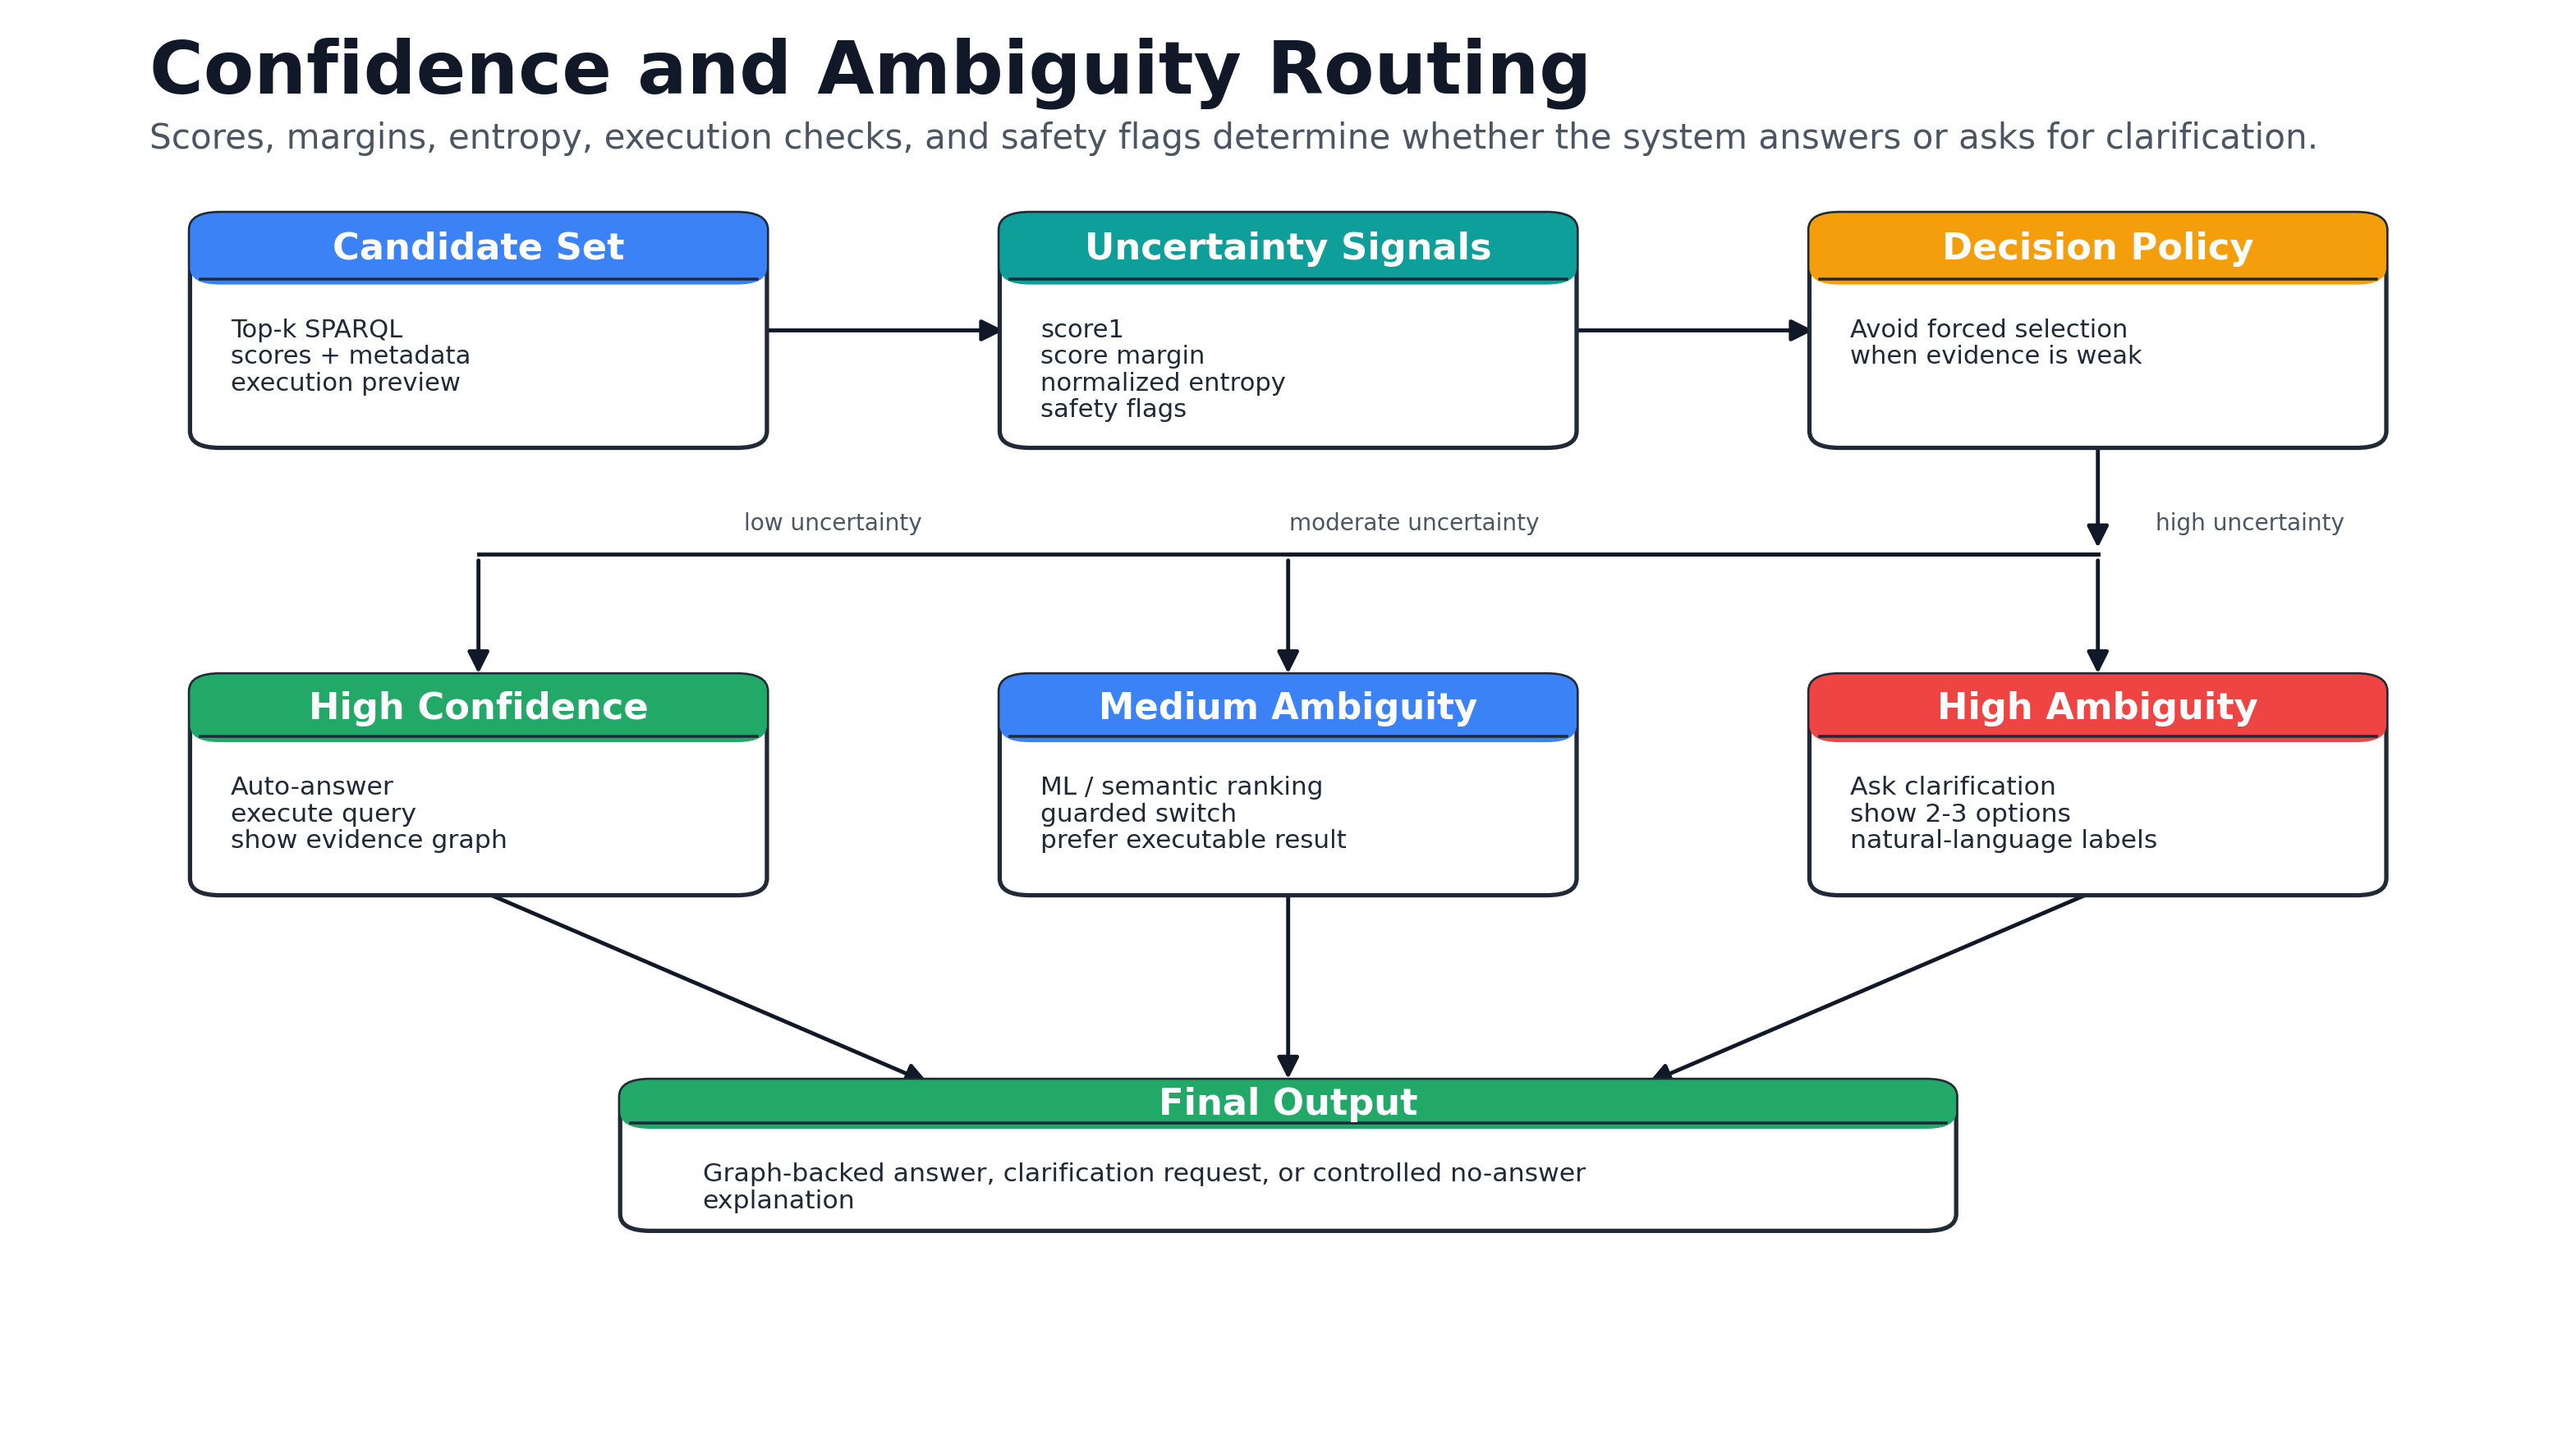
\includegraphics[width=0.92\textwidth]{confidence_ambiguity_routing.png}
    \caption{Confidence and ambiguity routing. Score, margin, entropy, execution checks, and safety flags determine whether the system answers automatically, applies guarded reranking, or asks the user for clarification.}
    \label{fig:confidence-ambiguity-routing}
\end{figure}

\begin{table}[htbp]
\centering
\caption{Signals used by the confidence and ambiguity router.}
\label{tab:confidence-signals}
\begin{tabularx}{\textwidth}{
>{\raggedright\arraybackslash}p{3.2cm}
>{\raggedright\arraybackslash}p{5.2cm}
>{\raggedright\arraybackslash}X
}
\toprule
\textbf{Signal} & \textbf{Interpretation} & \textbf{Typical action} \\
\midrule
High top score & The selected candidate is strongly preferred. & Candidate may be eligible for auto-answer. \\
Small margin & Top candidates are close. & Prefer guarded reranking or clarification. \\
High entropy & Candidate probabilities are diffuse. & Treat as uncertainty and inspect alternatives. \\
Safety flags & Contract, scope, shape, or capability mismatch is detected. & Block auto-answer or ask for clarification. \\
Empty result & Query executes but returns no rows. & Penalize candidate or avoid final answer. \\
Shape mismatch & Query result shape differs from requested answer type. & Penalize, rerank, or clarify. \\
\bottomrule
\end{tabularx}
\end{table}

The router has three operating regimes. In high-confidence cases, the selected candidate has a strong score, acceptable margin, no blocking safety flags, and executable graph evidence; the system answers automatically. In medium-uncertainty cases, the system may apply guarded ML selection and execution-aware checks. In high-ambiguity cases, the system shows two or three natural-language alternatives and asks the user to choose.

In the final user-testing version, slow fallback behavior is also converted into a clarification outcome. If no deterministic route is available and the LLM path exceeds the interactive budget, the router produces a small set of supported graph-backed alternatives instead of continuing to wait. This makes latency part of the reliability policy: an answer that cannot be selected quickly and safely is not forced.

\section{Execution Layer and Answer Synthesis}
\label{sec:execution-answer-synthesis}

After a query is selected, it is executed against the True Demand graph. The preferred runtime mode uses an Apache Jena Fuseki SPARQL endpoint because the graph can remain loaded and indexed during repeated querying. For local development or fallback execution, the system can use RDFLib over the Turtle graph file.

\begin{table}[htbp]
\centering
\caption{Execution modes supported by the system.}
\label{tab:execution-modes}
\begin{tabularx}{\textwidth}{p{3.5cm} p{4cm} X}
\toprule
\textbf{Mode} & \textbf{Role} & \textbf{Practical implication} \\
\midrule
Fuseki endpoint & Executes SPARQL over the loaded True Demand graph. & Suitable for interactive UI use and repeated queries. \\
RDFLib local graph & Parses and executes queries locally from the Turtle graph. & Useful for fallback and local debugging, but slower for repeated execution. \\
Preview execution & Executes candidate queries before final selection in selected modes. & Helps avoid empty or shape-inconsistent answers. \\
\bottomrule
\end{tabularx}
\end{table}

Execution returns rows, graph errors, or an empty result. These outputs are not treated as a passive final step. They are part of the reliability logic. A query that returns no evidence should not be presented as a successful high-confidence answer without qualification.

The answer synthesis module converts result rows into natural language. It must respect the expected answer shape. A grouped breakdown should be summarized as grouped results, not converted into a top-one answer unless the user explicitly asked for the highest, lowest, maximum, or minimum value.

\begin{table}[htbp]
\centering
\caption{Answer-shape handling during synthesis.}
\label{tab:answer-shape-synthesis}
\begin{tabularx}{\textwidth}{
>{\raggedright\arraybackslash}p{3.2cm}
>{\raggedright\arraybackslash}p{4.5cm}
>{\raggedright\arraybackslash}X
}
\toprule
\textbf{Question type} & \textbf{Expected result shape} & \textbf{Answer behavior} \\
\midrule
Scalar count & One row with a count value. & Report the count directly. \\
Grouped breakdown & Multiple rows with group variables and metric values. & Summarize the grouped results and preserve the table/evidence. \\
Ranking question & Ordered rows or explicit max/min aggregation. & Report the highest/lowest result and optionally supporting context. \\
List lookup & One column or small table of labels. & List returned values or summarize count and examples. \\
No result & Empty row set. & State that no graph-backed answer was found. \\
\bottomrule
\end{tabularx}
\end{table}

This stage closes the loop between query selection and user-facing answer quality. Even a correct query can be presented incorrectly if answer synthesis ignores the requested shape.

\section{User Interface and Visual Walkthrough}
\label{sec:user-interface}

The user interface is implemented as a Streamlit application. Its role is not only to collect a question and display an answer, but also to expose the system's decision process at the right level of detail. The interface supports natural-language question entry, validated examples, a guided question builder, a searchable Digital Reference ontology browser, clarification choices, answer synthesis, evidence graph visualization, feedback, and deployment diagnostics.

The user-testing version also refines the behavior of clarification choices. When a user selects a supported clarification option, the selected graph query is executed immediately and the answer is shown below, instead of copying the option back into the question box and requiring a second Ask action. Loading states are kept visually stable so that the page does not appear blurred or disabled while the backend is working.

Figure~\ref{fig:ui-main-question} shows the main question-entry view. The user can type a free natural-language question, but the interface also provides controlled alternatives through the question guide. This is important because the target user should not need to know SPARQL, while the system should still guide users toward graph-supported questions when possible.

\begin{figure}[!ht]
    \centering
    \includegraphics[width=0.78\textwidth]{figures/main-question.png}
    \caption{Main question-entry view in the Streamlit application. Users can ask a free natural-language question, while the question guide remains available for graph-supported examples and controlled question construction.}
    \label{fig:ui-main-question}
\end{figure}

The question guide exposes four complementary entry points. Validated examples provide known working questions. The guided builder allows users to compose a question by selecting only supported topic--metric--breakdown combinations. The available-topics view summarizes what kinds of questions the graph can answer. The Digital Reference tab exposes deterministic ontology definition lookup. Figure~\ref{fig:ui-question-guide-modes} groups these modes together.

\begin{figure}[!ht]
    \centering
    \begin{minipage}[t]{0.48\textwidth}
        \centering
        \includegraphics[width=\linewidth]{figures/question-guide-examples.png}\\[-1mm]
        \small (a) Validated examples
    \end{minipage}\hfill
    \begin{minipage}[t]{0.48\textwidth}
        \centering
        \includegraphics[width=\linewidth]{figures/question-guide-examples-guided-builder.png}\\[-1mm]
        \small (b) Guided builder
    \end{minipage}
    
    \vspace{2mm}
    
    \begin{minipage}[t]{0.48\textwidth}
        \centering
        \includegraphics[width=\linewidth]{figures/question-guide-examples-available-topics.png}\\[-1mm]
        \small (c) Available topics
    \end{minipage}\hfill
    \begin{minipage}[t]{0.48\textwidth}
        \centering
        \includegraphics[width=0.78\linewidth]{figures/question-guide-examples-digital-reference.png}\\[-1mm]
        \small (d) Digital Reference browser
    \end{minipage}
    \caption{Question-guide modes in the Streamlit interface. Users can choose validated examples, construct supported questions through the guided builder, inspect available graph topics, or browse Digital Reference ontology terms.}
    \label{fig:ui-question-guide-modes}
\end{figure}

The Digital Reference tab is intentionally separated from the KG analytics flow: ontology definition questions are answered from the DR ontology index, while analytical questions are answered from the True Demand KG.

After execution, the application presents both the answer and the reason why the answer was selected. Figure~\ref{fig:ui-main-answer} shows a high-confidence deterministic answer. The explanation states that the capability resolver found a single supported metric, dimension, aggregation, and graph path. This explicitly communicates that the LLM was skipped and that the answer is backed by graph execution.

\begin{figure}[!ht]
    \centering
    \includegraphics[width=0.72\textwidth]{figures/main-answer.png}
    \caption{User-facing answer and explanation. The interface reports the route decision, confidence score, row evidence, and the reasoning behind the selected answer.}
    \label{fig:ui-main-answer}
\end{figure}

The UI separates business-facing information from technical details. The default view uses natural-language interpretations and readable answers. The technical SPARQL query, candidate diagnostics, and developer controls are available through expandable sections. This separation is important because the target user may not know SPARQL, while developers and evaluators still need access to the internal decision process.

\begin{table}[!ht]
\centering
\caption{Main UI elements and their purpose.}
\label{tab:ui-elements}
\scriptsize

\begin{tabularx}{\textwidth}{
>{\raggedright\arraybackslash}p{3.5cm}
>{\raggedright\arraybackslash}p{4cm}
>{\raggedright\arraybackslash}X
}
\toprule
\textbf{UI element} & \textbf{Purpose} & \textbf{User benefit} \\
\midrule
Question input & Allows free natural-language questions. & No SPARQL knowledge required. \\
Guided examples & Shows graph-supported question patterns. & Reduces unsupported or underspecified questions. \\
Autocomplete suggestions & Suggests graph-aware metrics and dimensions. & Helps users phrase answerable questions. \\
Clarification cards & Shows plausible interpretations in natural language. & Avoids forced wrong answers. \\
Technical SPARQL expander & Shows generated and selected query. & Supports debugging and expert inspection. \\
Answer panel & Presents the synthesized graph-backed answer. & Provides a business-readable output. \\
Evidence graph & Shows entities and relationships related to the answer. & Increases trust and explainability. \\
Feedback controls & Allows the user to mark whether the answer was useful. & Supports iterative evaluation. \\
Developer/status panel & Shows backend, model, graph, and routing configuration. & Supports reproducibility and deployment debugging. \\
\bottomrule
\end{tabularx}
\end{table}
\normalsize

\section{Ontology and Evidence Visualization}
\label{sec:ontology-evidence-visualization}

The final interface uses two integrated graph visualizations. The first is a schema-level graph overview that helps users and developers inspect the main True Demand classes and relationships. The second is a query-specific answer evidence graph that shows the smaller subgraph related to the selected answer. Earlier in development, WebVOWL was used as an external ontology viewer to inspect the first schema representation; it is not part of the final user-facing system and is therefore not used as the main thesis screenshot.

Figure~\ref{fig:ui-schema-overview-details} shows the integrated schema overview. Users can zoom, pan, click nodes, and inspect outgoing and incoming relationships. This view is useful for understanding the graph structure, but it is still a schema-level overview. It does not replace SPARQL execution over the full 1.16 million-triple graph.

\begin{figure}[!ht]
    \centering
    \begin{minipage}[t]{0.48\textwidth}
        \centering
        \includegraphics[width=\linewidth]{figures/schema1.png}\\[-1mm]
        \small (a) Schema-level graph overview
    \end{minipage}\hfill
    \begin{minipage}[t]{0.48\textwidth}
        \centering
        \includegraphics[width=\linewidth]{figures/schema3.png}\\[-1mm]
        \small (b) Node-level relationship inspection
    \end{minipage}
    \caption{Integrated schema-level graph visualization. The overview shows the main True Demand ontology classes and relationships, while clicking a node opens available identifiers and incoming/outgoing relationships.}
    \label{fig:ui-schema-overview-details}
\end{figure}

The answer evidence graph is different. It is generated after a question is answered and contains only the entities and predicates relevant to the selected query and returned rows. Figure~\ref{fig:ui-answer-evidence-graph} shows this query-specific evidence view. It helps users verify that the response came from graph execution and not from unsupported free-text generation.

\begin{figure}[!ht]
    \centering
    \includegraphics[width=0.74\textwidth]{figures/main-answer-graph2.png}
    \caption{Query-specific answer evidence graph. The visualization shows the graph relationships used by the selected query together with a preview of the returned answer row.}
    \label{fig:ui-answer-evidence-graph}
\end{figure}

\section{Developer and Deployment Controls}
\label{sec:developer-deployment-controls}

The deployed system includes lightweight status diagnostics and a separate confidence-routing dashboard. The status panel verifies that the schema, ranker model, graph backend, and LLM configuration are available. This is useful for deployment because a missing model file, unreachable Fuseki endpoint, or missing LLM credential would otherwise appear to the user as a generic application failure.

These diagnostics are particularly important for deployment because local and deployed runs may differ in their graph backend mode. For example, a local run may use a Fuseki endpoint, while a deployed run may load a Turtle file inside the container unless the endpoint is configured explicitly. The status panel and guided-example availability therefore act as practical checks that the deployed runtime is using the same graph, schema, DR ontology, model, and validated query assets as the local system.

The graph overview page also contains a compact natural-language description of the graph, its scale, and the types of questions users can ask. Figure~\ref{fig:ui-overview-status} shows the status and overview documentation together. This view is intentionally separate from the confidence dashboard: the overview explains what the graph contains, while the confidence dashboard explains how the system behaves during evaluation.

\begin{figure}[!ht]
    \centering
    \begin{minipage}[t]{0.32\textwidth}
        \centering
        \includegraphics[width=\linewidth]{figures/system-status.png}\\[-1mm]
        \small (a) Runtime status
    \end{minipage}\hfill
    \begin{minipage}[t]{0.32\textwidth}
        \centering
        \includegraphics[width=\linewidth]{figures/true-demand-overview1.png}\\[-1mm]
        \small (b) Graph overview
    \end{minipage}\hfill
    \begin{minipage}[t]{0.32\textwidth}
        \centering
        \includegraphics[width=\linewidth]{figures/true-demand-overview2.png}\\[-1mm]
        \small (c) Measures and examples
    \end{minipage}
    \caption{Status and graph-overview documentation. The application exposes runtime availability checks, graph scope, available question types, schema scale, example questions, and usage guidance.}
    \label{fig:ui-overview-status}
\end{figure}

The confidence-routing dashboard is an evaluation-oriented view. It exposes aggregate routing behavior and error cases, including high-confidence wrong examples, family filters, safety flags, and bucket composition. This dashboard is useful for developers and evaluators, but it is not intended as the primary business-user interface.

\begin{figure}[!ht]
    \centering
    \includegraphics[width=0.68\textwidth]{figures/confidence-routing.png}
    \caption{Confidence-routing case browser. Evaluators can filter high-confidence wrong examples by family, score, safety flags, and other diagnostic attributes.}
    \label{fig:ui-confidence-case-browser}
\end{figure}

\section{Summary}
\label{sec:architecture-summary}

The True Demand KGQA architecture combines deterministic and probabilistic components. Direct graph-supported routing handles frequent answerable questions without using the LLM. The LLM is reserved for cases where candidate generation is needed. Candidate queries are then validated, featurized, ranked, checked for execution behavior, and routed through confidence and ambiguity logic. The selected query is executed against the knowledge graph, and the result is synthesized into a natural-language answer with optional evidence visualization.

This architecture addresses the main weaknesses of a naive LLM-to-SPARQL system. It reduces unnecessary LLM usage, avoids unsupported graph paths, separates query generation from query selection, penalizes empty or shape-inconsistent candidates, and gives the user a clarification path when automatic selection would be unreliable. The user interface makes this behavior visible through autocomplete, clarification options, technical SPARQL expanders, answer evidence graphs, and developer diagnostics.





\chapter{Methodology}
\label{chap:methodology}

\section{Benchmark Construction}
\label{sec:benchmark-construction}

The evaluation uses two complementary benchmark views. The first view isolates the LLM-based query-selection problem. In this setting, each natural-language question is associated with a candidate set of SPARQL queries generated by the LLM or retrieved from validated examples. The task is to select the candidate that best matches the intended interpretation. This benchmark is useful for measuring candidate generation coverage, Top-1 selection accuracy, and the effect of schema-aware and ML-based ranking.

The second view evaluates the complete user-facing system. In this setting, the system is allowed to use all available routing mechanisms: deterministic graph-supported templates, DR ontology definition lookup, advisory templates, LLM candidate generation, guarded ML reranking, execution checks, and answer synthesis. This benchmark measures the final answer that a user would see, not only whether a particular candidate query was selected.

The final system benchmark contains 1000 questions. It was constructed to cover three usage modes:

\begin{itemize}
    \item \textbf{KG analytics questions}: 800 questions over True Demand data, covering current demand, future demand, regional demand, vehicle sales, shortage, inventory, order cancellation, autonomous-driving indicators, and catalog lookup.
    \item \textbf{DR ontology questions}: 150 definition-style questions asking for the meaning of ontology classes and properties.
    \item \textbf{Advisory questions}: 50 graph-grounded questions asking for planning signals, monitoring priorities, or risk indicators based on available graph results.
\end{itemize}

The KG analytics questions were designed to include both simple and compositional requests. Examples include grouped breakdowns, total counts, average values, top-value questions, survey-scope filters, and multi-dimensional combinations. The ontology questions test whether users can ask about the conceptual model without knowing ontology identifiers. The advisory questions test whether the system can transform graph results into conservative data-grounded recommendations.

\begin{table}[htbp]
\centering
\caption{Evaluation views used in the thesis.}
\label{tab:evaluation-views}
\small
\begin{tabularx}{\textwidth}{
>{\raggedright\arraybackslash}p{3.5cm}
>{\raggedright\arraybackslash}p{4.2cm}
>{\raggedright\arraybackslash}X
}
\toprule
\textbf{Evaluation view} & \textbf{Scope} & \textbf{Purpose} \\
\midrule
LLM selection benchmark & Candidate sets for LLM-needed questions & Measures candidate coverage, raw selection, schema-aware selection, and ML reranking. \\
Fallback subset benchmark & Questions not answered deterministically in the final system & Measures raw/schema/ML selection on the exact questions that enter the fallback layer. \\
Full-system benchmark & 1000 mixed user-facing questions & Measures end-to-end answer correctness, routing, LLM-call reduction, and practical system behavior. \\
DR ontology benchmark & 300 ontology definition questions & Measures deterministic ontology-definition lookup without LLM calls. \\
\bottomrule
\end{tabularx}
\end{table}

\section{Gold Benchmark Validation and Repair}
\label{sec:gold-benchmark-validation-repair}

The final evaluation depends on the quality of the benchmark itself. If a gold SPARQL query is wrong, empty for the wrong reason, or mapped to a question that it does not actually answer, the measured system accuracy becomes misleading. For this reason, the 1000-question KG benchmark was not used as a raw generated dataset. It was validated and repaired before the final system evaluation.

The validation process combined manual inspection and automated checks. First, each gold query was checked for syntactic validity and executable behavior against the True Demand RDF graph. Queries were executed through the same graph backend used by the application, including Fuseki when available. The validation script recorded whether the query executed, how many rows it returned, whether the result shape matched the expected answer type, and whether the question belonged to the expected analytical family. This automatically identified queries that were invalid, returned no rows, or looked suspicious because the requested metric, grouping dimension, or answer shape did not match the query.

Second, the suspicious and representative cases were manually inspected. Approximately half of the 1000 benchmark questions were checked manually either directly through Fuseki result inspection or through the detailed audit sheets used during system evaluation. This manual step was especially important for questions where a query returned rows but still might be semantically wrong. For example, a query can return a non-empty result while grouping by region although the question asks for survey group, or it can return a top-ranked value although the question asks for a full breakdown. These cases cannot be validated by row count alone.

The manual validation followed a consistent procedure:

\begin{enumerate}
    \item inspect the natural-language question and identify the requested metric, scope, grouping dimension, aggregation, and answer shape;
    \item execute the gold SPARQL query in Fuseki or through the local RDF graph;
    \item inspect whether the returned rows were non-empty and whether they matched the requested interpretation;
    \item mark the gold query as correct, probably correct, or incorrect;
    \item repair incorrect gold queries when the graph contained a better supported path;
    \item keep notes explaining whether the problem was an empty result, a wrong path, a wrong aggregation, a missing scope, or an answer-shape mismatch.
\end{enumerate}

This process exposed several concrete benchmark problems. Some autonomous-driving questions referred to survey-specific classes that were not populated in the graph, while the actual graph used a shared \texttt{AutonomousDrivingDevelopment} class with survey information represented differently. Some vehicle-sales questions used the wrong actual/forecast filter or counted observations instead of summing \texttt{unitsSold}. Some future-demand and order-cancellation questions returned only the highest category even though the question asked for a breakdown across categories. These were repaired by changing the gold query, and in a few cases by changing the question wording to match the graph-supported interpretation.

\begin{table}[htbp]
\centering
\caption{Benchmark validation checks applied before the final evaluation.}
\label{tab:benchmark-validation-checks}
\small
\begin{tabularx}{\textwidth}{
>{\raggedright\arraybackslash}p{3.2cm}
>{\raggedright\arraybackslash}p{3.1cm}
>{\raggedright\arraybackslash}X
}
\toprule
\textbf{Validation layer} & \textbf{Applied to} & \textbf{Purpose} \\
\midrule
SPARQL syntax and prefix check & All KG gold queries & Detect malformed queries, unresolved prefixes, and queries that cannot be parsed. \\
Fuseki / RDF execution & Manual sample and flagged queries & Verify that the query actually runs against the loaded True Demand graph and inspect returned rows. \\
Empty-result inspection & Queries with zero rows & Distinguish genuinely absent data from unsupported or overly specific gold paths. \\
Answer-shape check & All automatically processed rows & Verify that count, sum, average, top-value, raw-list, and grouped-breakdown questions return the expected result structure. \\
Manual semantic audit & Approximately half of the 1000-question benchmark & Check whether non-empty query results actually answer the natural-language question. \\
Result-signature comparison & Remaining KG analytics audit rows & Compare selected-query outputs against repaired gold-query outputs when no unchanged manual label was available. \\
\bottomrule
\end{tabularx}
\end{table}

The remaining half of the benchmark was validated automatically through execution and semantic diagnostics. This included syntactic parsing, non-empty execution checks where appropriate, expected-family checks, answer-shape checks, and result-signature comparisons. For the final full-system audit, KG analytics answers were labeled by comparing the selected query's result signature against the repaired gold query result signature when no unchanged previous manual label was available. DR ontology definition questions were evaluated through deterministic ontology lookup behavior, and advisory questions were evaluated as graph-backed recommendations with non-empty evidence rows and conservative answer synthesis.

The final benchmark validation therefore used a layered approach rather than a single weak criterion. Manual Fuseki inspection was used for the difficult and suspicious cases, while automatic validation ensured that the remaining benchmark rows were executable and consistent with their expected result shape. This does not make the benchmark perfect in a formal semantic sense, but it makes it substantially more reliable than an unverified generated benchmark and provides an audit trail for the reported accuracy values.

\section{Evaluation Metrics}
\label{sec:evaluation-metrics}

The evaluation distinguishes between several metrics because they answer different questions.

\textbf{Top-1 selection accuracy} measures whether the first selected candidate query is correct. This is the main metric for the query-selection component. It is computed only on candidate sets where generated alternatives exist.

\textbf{Any-correct candidate coverage} measures whether at least one candidate in the generated set is correct. This evaluates candidate generation rather than selection. High Any-Correct with lower Top-1 accuracy indicates that the correct query is often generated but not always selected.

\textbf{Execution-plausible selected-query rate} measures whether the selected query executed without an error and returned graph rows. It is less strict than Top-1 selection accuracy because it does not require the selected query to be the canonical repaired gold query. Instead, it asks whether the selected query is executable and produces graph evidence. This metric is useful because multiple SPARQL queries may be semantically close or may produce an acceptable user-facing answer even when they are not identical to the gold query. However, execution plausibility alone is not sufficient for correctness: a non-empty query can still answer the wrong business question. Therefore, it is reported as an intermediate execution signal, not as a replacement for strict selection accuracy or manual answer-level correctness.

\textbf{Answer-level correctness} measures whether the final user-facing answer is correct. This is used for the full system because a final answer can be correct even when the selected query is not identical to a canonical gold query, for example when multiple semantically equivalent queries produce the same answer.

\textbf{LLM-call reduction} measures how many questions avoid an LLM call through deterministic routing. With an assumed cost of EUR 0.20 per LLM call, the cost of the final system can be compared against an all-LLM baseline.

\textbf{Human SPARQL difficulty} is used for error analysis. Incorrect final-system answers are classified according to how difficult it would be for a knowledgeable human to formulate the correct SPARQL query or validate the graph-grounded answer: easy, medium, or hard. This analysis helps distinguish avoidable system mistakes from genuinely schema-dependent or ambiguous graph-composition problems.

\begin{table}[htbp]
\centering
\caption{Metrics used in the final evaluation.}
\label{tab:evaluation-metrics}
\small
\begin{tabularx}{\textwidth}{
>{\raggedright\arraybackslash}p{3.6cm}
>{\raggedright\arraybackslash}X
}
\toprule
\textbf{Metric} & \textbf{Interpretation} \\
\midrule
Top-1 selection accuracy & Correct candidate selected as the first query. \\
Any-correct coverage & At least one correct candidate exists in the candidate set. \\
Execution-plausible selected query & Selected query executes without error and returns graph rows. \\
Answer-level correctness & Final answer judged correct in the system audit. \\
LLM-call reduction & Share of questions answered without LLM calls. \\
Human SPARQL difficulty & Estimated difficulty of manually writing the correct query for failed cases. \\
\bottomrule
\end{tabularx}
\end{table}

\section{Ambiguity Measurement}
\label{sec:ambiguity-measurement}

Ambiguity is measured at the candidate-set level. The key assumption is that a natural-language question is not evaluated in isolation, but together with the set of candidate SPARQL queries produced for it. Let a question \(Q\) have a candidate set

\[
C(Q) = \{q_1, q_2, \ldots, q_n\},
\]

where each \(q_i\) is a candidate query and \(n\) is the number of generated candidates. A ranking method assigns each candidate a score \(s_i\). This score may come from the raw LLM ordering, a schema-aware scoring function, or the ML reranker. Higher scores indicate that the candidate is considered more likely to match the intended interpretation of the question.

To compare candidates within the same question, the scores are converted into a probability-like distribution. In the implementation, this can be done through a softmax transformation:

\[
p_i =
\frac{\exp(s_i / \tau)}
{\sum_{j=1}^{n} \exp(s_j / \tau)},
\]

where \(\tau\) is a temperature parameter controlling how sharply score differences are translated into probabilities. A lower temperature makes the largest score dominate more strongly, while a higher temperature produces a flatter distribution. The resulting values satisfy:

\[
\sum_{i=1}^{n} p_i = 1, \qquad p_i \geq 0.
\]

The ambiguity of the candidate set is then estimated using Shannon entropy:

\[
H(Q) = - \sum_{i=1}^{n} p_i \log(p_i),
\]

where \(Q\) is the natural-language question, \(n\) is the number of candidates, and \(p_i\) is the normalized score assigned to candidate \(i\). The maximum entropy depends on the number of candidates. To make values comparable across questions with different candidate-set sizes, the normalized entropy is computed as:

\[
H_{\mathrm{norm}}(Q) =
\frac{H(Q)}{\log(n)}.
\]

This gives \(H_{\mathrm{norm}}(Q) \in [0,1]\) for candidate sets with \(n > 1\). A value close to 0 indicates that one candidate dominates the score distribution. A value close to 1 indicates that the scores are spread more evenly across candidates, meaning that the ranking model has no clear preference.

In addition to entropy, the system also uses the score margin between the two highest-ranked candidates:

\[
\Delta(Q) = s_{(1)} - s_{(2)},
\]

where \(s_{(1)}\) and \(s_{(2)}\) are the highest and second-highest candidate scores. A large margin indicates that the top candidate is clearly preferred by the scoring model. A small margin indicates that the first and second candidates are close competitors. Entropy and margin are complementary: entropy summarizes the whole candidate distribution, while the margin focuses on the local competition at the top of the ranking.

For analysis, candidate sets can be grouped into ambiguity regimes:

\[
\text{regime}(Q) =
\begin{cases}
\text{low ambiguity}, & H_{\mathrm{norm}}(Q) \leq \theta_1, \\
\text{medium ambiguity}, & \theta_1 < H_{\mathrm{norm}}(Q) \leq \theta_2, \\
\text{high ambiguity}, & H_{\mathrm{norm}}(Q) > \theta_2.
\end{cases}
\]

The thresholds \(\theta_1\) and \(\theta_2\) are not treated as universal constants. They can be defined by quantiles for diagnostic analysis or calibrated empirically on validation data for routing. This is important because the absolute scale of entropy depends on the scoring method, candidate generation strategy, and temperature.

In practice, this entropy measure should be interpreted as \emph{model uncertainty over candidate selection}, not as a perfect measure of the intrinsic ambiguity of the natural-language question. A high entropy score can occur because the question is genuinely ambiguous, because the generated candidates are near duplicates, or because the ranker cannot distinguish structurally similar queries. Conversely, a low entropy score can still be wrong if the ranker is confidently selecting a semantically incorrect candidate.

An important limitation is that entropy over individual SPARQL strings can overestimate ambiguity when several candidates are execution-equivalent. For example, two queries may use different variable names or reorder triple patterns but return the same projected rows. To make this explicit, the implementation includes a diagnostic execution-signature clustering step. For each candidate \(q_i\), a preview execution signature \(\sigma(q_i)\) can be defined from its projected columns, row count, and preview rows. Candidates with the same signature are grouped into clusters \(G_k\), and their probabilities are summed:

\[
P_k = \sum_{q_i \in G_k} p_i.
\]

The clustered entropy is then:

\[
H_{\mathrm{sig}}(Q) =
- \sum_{k=1}^{m} P_k \log(P_k),
\qquad
H_{\mathrm{sig,norm}}(Q) =
\frac{H_{\mathrm{sig}}(Q)}{\log(m)}.
\]

Here, \(m\) is the number of distinct execution signatures. This diagnostic does not replace the main entropy measure, because execution previews are not always available before final selection and equivalent row previews do not prove full semantic equivalence. However, it makes the limitation transparent: entropy should be interpreted over candidate alternatives, and execution-equivalent alternatives should not be over-read as genuine user ambiguity.

For this reason, entropy is not used as a standalone truth signal. It is used as a routing and diagnostic signal together with confidence, margin, schema features, answer shape, execution behavior, and candidate source. The final system uses this logic to decide when to answer automatically, when to apply guarded ML reranking, and when clarification or conservative fallback is more appropriate.

This connects the theoretical measure to the implemented system. Low-uncertainty candidate sets are candidates for automatic answering if execution checks also succeed. Medium-uncertainty candidate sets are where the guarded ML reranker is most useful, because several plausible candidates exist but there may still be enough signal to select one. High-uncertainty candidate sets indicate that automatic selection is less reliable; in these cases, the system should prefer clarification, abstention, or conservative fallback rather than forcing a potentially wrong query. Thus, entropy is not presented as a replacement for validation. It provides a principled uncertainty signal that complements the system's graph-based safety checks.

\section{System-Level Evaluation}
\label{sec:system-level-evaluation-method}

The full-system benchmark was executed through the same pipeline used by the Streamlit application. Each question first passed through the deterministic routing layer. If a supported graph capability, DR ontology definition, or advisory route was available, the system answered without LLM generation. Otherwise, the question entered the LLM fallback layer, where candidates were generated or retrieved, validated, reranked, executed, and synthesized into a final answer.

The final audit file records the question ID, question text, topic, expected route, selected source, selected query, row count, answer text, and correctness label. Correctness was evaluated at the answer level. This means that the final answer was judged according to whether it answered the user question, not only whether the selected SPARQL query matched one canonical query string. For KG analytics rows without an unchanged previous manual label, the final label was produced by comparing the result signature of the selected query with the result signature of the repaired gold query. This made the audit stricter than a purely text-based answer review. For DR ontology and advisory rows, deterministic route-specific checks were used because those answers are not ordinary KG analytics queries.


\chapter{Experiments and Results}
\label{chap:experiments-results}

\section{Baseline Selection Results}
\label{sec:baseline-selection-results}

The first experiment evaluates the LLM candidate-generation and selection pipeline independently of deterministic routing. On the repaired 1000-question KG selection benchmark, the raw LLM candidate order achieved 51.7\% Top-1 accuracy, while Any-Correct coverage reached 81.4\%. This means that in most cases the correct query was present somewhere in the generated candidate set, but the first selected candidate was often not the correct interpretation.

This result confirms the core motivation of the thesis: the main bottleneck is not only query generation, but query selection under ambiguity. If the correct query appears in the candidate set but is not selected, improving the ranking and routing layer can improve reliability without necessarily requiring more LLM calls.

The gap between Top-1 accuracy and Any-Correct coverage is the most important observation in this experiment. A Top-1 value of 51.7\% means that the raw candidate order produced by the LLM is not reliable enough to be executed blindly. However, the Any-Correct value of 81.4\% means that the LLM still frequently generated a correct query somewhere in the candidate set. The system is therefore not only failing because the LLM cannot express the graph query at all. It also fails because several plausible candidates are generated and the wrong one is ranked first. This justifies treating KGQA as a candidate-selection problem rather than as a single-query generation problem.

\begin{table}[htbp]
\centering
\caption{LLM-only selection benchmark results on the 1000-question KG benchmark.}
\label{tab:llm-selection-baseline-results}
\small
\begin{tabularx}{\textwidth}{
>{\raggedright\arraybackslash}X
>{\raggedleft\arraybackslash}p{1.7cm}
>{\raggedleft\arraybackslash}p{1.6cm}
>{\raggedleft\arraybackslash}p{1.9cm}
>{\raggedleft\arraybackslash}p{1.8cm}
}
\toprule
\textbf{Mode} & \textbf{Questions} & \textbf{Top-1} & \textbf{Any Correct} & \textbf{Gen. fail.} \\
\midrule
Raw LLM order & 1000 & 51.7\% & 81.4\% & 18.6\% \\
Schema / semantic selection & 1000 & 48.2\% & 81.4\% & 18.6\% \\
Guarded ML selection & 1000 & 53.6\% & 81.4\% & 18.6\% \\
\bottomrule
\end{tabularx}
\end{table}

The schema-only result is lower than raw LLM ordering in this benchmark. This is an important finding. Schema validity alone is not sufficient for semantic correctness: a query can use valid classes and relationships while still answering the wrong analytical question. This motivates the use of answer-shape features, execution-aware validation, and ML-based reranking rather than relying only on schema matching.

This result also explains why a purely ontology-constrained system is not enough for the True Demand graph. The ontology can say that a class, property, or path is valid, but it cannot always decide whether the query matches the user's business intent. For example, a query that counts records may be structurally valid, but it is not correct if the user asked for a demand value. Similarly, a query over future demand may be schema-valid but wrong for a current-demand question. The decrease from 51.7\% to 48.2\% shows that schema information can even hurt selection when it over-prioritizes structurally clean but semantically mismatched candidates.

This does not contradict the use of schema-derived features inside the ML reranker. The difference is that schema-only selection treats structural validity as the main decision criterion, while the guarded ML model treats schema validity as one signal among many. The ML feature vector also contains answer-shape indicators, aggregation type, selected variables, candidate source, scope/provenance cues, and safety flags. This allows the model to down-weight schema-valid but intent-mismatched candidates, such as a valid count query when the user asked for a grouped demand value. In other words, schema information is useful as evidence, but harmful when used as the complete objective. On the repaired benchmark, this produces a smaller but still positive strict-selection gain: guarded ML improves Top-1 from 51.7\% to 53.6\%.

\section{ML Reranking Results}
\label{sec:ml-reranking-results}

The ML reranker was trained on grouped candidate-query examples, where candidates belonging to the same natural-language question form a ranking group. The model uses query-plan and schema-derived features, including aggregation type, grouping behavior, selected variables, expected domains, source metadata, and semantic coverage signals. The model is applied in a guarded manner: it does not override the selected candidate unless score, margin, and rank constraints are satisfied.

Before the final repaired benchmark was fixed, a separate calibration split was used during model development to choose a guarded reranking configuration. However, the final reported selection result is the repaired 1000-question benchmark below. This avoids mixing calibration diagnostics with the final evaluation.

The repaired 1000-question candidate set was analyzed with detailed failure counts. Raw LLM ordering selected the correct candidate for 517 questions. Schema-only selection selected 482 correctly, confirming that structural validity alone can over-prioritize semantically wrong candidates. Guarded ML selected 536 correctly, improving over raw ordering by 19 questions. Candidate coverage was 81.4\% for all three settings because the candidate set was the same; only the selection strategy changed.

\begin{table}[htbp]
\centering
\caption{Detailed selection results on the repaired 1000-question KG benchmark.}
\label{tab:repaired1000-selection}
\small
\begin{tabularx}{\textwidth}{
>{\raggedright\arraybackslash}X
>{\raggedleft\arraybackslash}p{1.5cm}
>{\raggedleft\arraybackslash}p{1.3cm}
>{\raggedleft\arraybackslash}p{1.8cm}
>{\raggedleft\arraybackslash}p{1.6cm}
>{\raggedleft\arraybackslash}p{1.6cm}
}
\toprule
\textbf{Mode} & \textbf{Questions} & \textbf{Top-1} & \textbf{Any Correct} & \textbf{Rank fail.} & \textbf{Gen. fail.} \\
\midrule
Raw LLM selection & 1000 & 51.7\% & 81.4\% & 296 & 186 \\
Schema-only selection & 1000 & 48.2\% & 81.4\% & 331 & 186 \\
Guarded ML selection & 1000 & 53.6\% & 81.4\% & 277 & 186 \\
\bottomrule
\end{tabularx}
\end{table}

Guarded ML therefore improves the strict selection layer by 1.9 percentage points over raw LLM ordering, corresponding to 19 additional correctly selected queries on the repaired 1000-question KG benchmark. This is a more conservative result than the earlier fallback diagnostic, because the gold benchmark was repaired and the evaluation contract became stricter. The Any-Correct value shows that candidate generation still leaves selection headroom: 814 questions contain a correct candidate somewhere in the candidate set, while guarded ML selects 536 of them as Top-1.

The repaired selection benchmark should be interpreted separately from the final answer-level benchmark. It is strict: a candidate is correct only when it matches the repaired gold query intent. It does not count cases where a different query produces an acceptable answer, and it does not include deterministic ontology lookup, direct graph templates, advisory routing, or answer synthesis. This explains why strict guarded-ML selection reaches 53.6\%, while the final hybrid system reaches 89.4\% answer-level accuracy.

The low schema-only result on the same repaired benchmark further supports the argument that ambiguity is semantic, not only structural. The difficult questions often involve competing domains, similar metrics, missing scope, or subtle differences between a grouped breakdown and a top-value query. Schema-only selection does not capture these distinctions well, while guarded ML can use additional features such as query shape, aggregation, selected variables, candidate source, and score margins.

To make this interpretation reproducible, the repository includes a schema-versus-ML diagnostic script. The script compares raw, schema-only, and guarded-ML analysis files and, when the ranker model is available, reports the largest absolute feature weights grouped into interpretable feature families. This provides an audit trail for the claim that the ML model succeeds by combining schema signals with non-schema signals, rather than by merely applying schema validation more strongly.

The full 1000-question KG selection benchmark is useful as a controlled scientific diagnostic, but it is not identical to the set of questions that actually reaches the LLM in the final hybrid system. In the final system, deterministic graph-supported templates, DR ontology lookup, and advisory templates answer many questions before LLM generation is attempted. Therefore, an additional fallback-subset analysis was computed. This analysis takes the 486 questions that the final system routed to the LLM fallback layer, maps them back to the repaired KG candidate benchmark where possible, and compares raw, schema-only, and guarded-ML selection only on that mapped fallback subset.

\begin{table}[htbp]
\centering
\caption{Selection results on the final-system LLM fallback subset.}
\label{tab:fallback-subset-selection}
\small
\setlength{\tabcolsep}{3pt}
\begin{tabularx}{\textwidth}{
>{\raggedright\arraybackslash}X
>{\raggedleft\arraybackslash}p{1.4cm}
>{\raggedleft\arraybackslash}p{1.35cm}
>{\raggedleft\arraybackslash}p{1.6cm}
>{\raggedleft\arraybackslash}p{1.8cm}
>{\raggedleft\arraybackslash}p{1.45cm}
>{\raggedleft\arraybackslash}p{1.45cm}
}
\toprule
\textbf{Mode} & \textbf{Q.} & \textbf{Top-1} & \textbf{Any Correct} & \textbf{Exec.-plaus.} & \textbf{Rank fail.} & \textbf{Gen. fail.} \\
\midrule
Raw LLM selection & 482 & 56.2\% & 82.8\% & 85.9\% & 128 & 83 \\
Schema-only selection & 482 & 53.7\% & 82.8\% & 81.7\% & 140 & 83 \\
Guarded ML selection & 482 & 58.7\% & 82.8\% & 86.1\% & 116 & 83 \\
\bottomrule
\end{tabularx}
\end{table}

Table~\ref{tab:fallback-subset-selection} is the most direct selection diagnostic for the deployed hybrid pipeline, because it evaluates only the questions that were not solved deterministically. Of the 486 final-system fallback questions, 482 could be mapped to repaired KG candidate IDs; the four unmatched questions were advisory-style fallback cases and are excluded from strict KG candidate selection. On this mapped fallback subset, guarded ML improves Top-1 selection from 56.2\% to 58.7\%, corresponding to 12 additional correctly selected candidates over raw LLM ordering. The Any-Correct value remains 82.8\% across modes because the generated candidate set is unchanged. Schema-only selection again performs worse than raw ordering, confirming that schema validity is a useful signal but an insufficient decision rule.

A second diagnostic evaluates the same selection problem with a less strict execution-oriented signal. The strict Top-1 metric asks whether the selected candidate is the repaired canonical gold candidate. The execution-plausible metric instead asks whether the selected candidate executed successfully and returned graph evidence. This is not the same as correctness, because a non-empty query may still answer the wrong question. However, it explains why strict selection scores can be substantially lower than final answer-level scores: the final system can still produce an acceptable answer when the selected query is executable, semantically close, or result-equivalent to the repaired gold query.

To avoid evaluating a model on the same examples used for training or threshold tuning, a clean train--tune--holdout split was created from the repaired benchmark. The split used 600 questions for training, 200 questions for tuning, and 200 untouched questions for holdout evaluation. Table~\ref{tab:holdout200-selection-exec} reports this holdout analysis. In addition to raw and schema-only selection, it compares a feature-rich non-parametric reranker with two XGBoost learning-to-rank objectives. These variants test whether grouped ranking objectives improve selection without changing the generated candidate set.

\begin{table}[htbp]
\centering
\caption{Strict and execution-plausible selection results on the 200-question repaired holdout split.}
\label{tab:holdout200-selection-exec}
\footnotesize
\setlength{\tabcolsep}{3pt}
\begin{tabularx}{\textwidth}{
>{\raggedright\arraybackslash}X
>{\raggedleft\arraybackslash}p{1.25cm}
>{\raggedleft\arraybackslash}p{1.25cm}
>{\raggedleft\arraybackslash}p{1.45cm}
>{\raggedleft\arraybackslash}p{1.65cm}
>{\raggedleft\arraybackslash}p{1.35cm}
>{\raggedleft\arraybackslash}p{1.35cm}
}
\toprule
\textbf{Mode} & \textbf{Q.} & \textbf{Top-1} & \textbf{Any Correct} & \textbf{Exec.-plaus.} & \textbf{Rank fail.} & \textbf{Gen. fail.} \\
\midrule
Raw LLM selection & 200 & 51.5\% & 81.5\% & 80.5\% & 60 & 37 \\
Schema-only selection & 200 & 46.5\% & 81.5\% & 76.5\% & 70 & 37 \\
Feature-rich non-parametric & 200 & 50.5\% & 81.5\% & 81.5\% & 62 & 37 \\
XGBoost pairwise LTR & 200 & 54.0\% & 81.5\% & 83.0\% & 55 & 37 \\
XGBoost NDCG LTR & 200 & 51.5\% & 81.5\% & 80.5\% & 60 & 37 \\
\bottomrule
\end{tabularx}
\end{table}

The holdout results show three important patterns. First, schema-only selection again performs worse than raw ordering, both in strict Top-1 accuracy and in execution plausibility. This confirms that selecting the most schema-compatible candidate is not enough. Second, feature-rich non-parametric reranking improves execution plausibility but does not improve strict Top-1 accuracy, which indicates that execution-friendly signals and canonical-query correctness are related but not identical. Third, the pairwise XGBoost learning-to-rank objective gives the best holdout result, improving strict Top-1 selection from 51.5\% to 54.0\% and execution-plausible selection from 80.5\% to 83.0\%. The gain is modest but clean: it is measured on an untouched holdout split and uses grouped candidate sets rather than tuning on the final evaluation rows.

The NDCG objective did not improve over raw ordering on this holdout. This suggests that the main bottleneck is not simply the tree objective or hyperparameter tuning, but the available semantic features and the quality of the generated candidate set. The reported system therefore keeps the ranking layer conservative: ML is useful, but it should be interpreted as a guarded selection aid rather than as a complete semantic judge.

The distinction between Top-1 and execution plausibility is central to interpreting the numbers. Top-1 is a strict scientific metric for candidate selection: the selected candidate must match the repaired gold intent. Execution plausibility is an operational metric: the selected query must execute and return rows. The former answers whether the selection model chose the canonical target; the latter answers whether the selected query produced graph evidence. Neither metric alone is sufficient. Strict Top-1 can undercount result-equivalent or acceptable alternatives, while execution plausibility can overcount non-empty but semantically wrong queries. For this reason, the thesis reports both, and keeps final system accuracy as a separate answer-level audit.

\section{Error Analysis}
\label{sec:error-analysis-results}

The final repaired full-system audit contains 106 incorrect answers out of 1000 questions. Of these, 11 occur in the deterministic route and 95 occur in the LLM fallback route. The audit did not leave any rows as unclear. Each incorrect row was also assigned a human SPARQL difficulty label. This label estimates how difficult it would be for a knowledgeable human analyst, with access to the schema and graph, to formulate and validate the correct query manually. It does not measure whether the final answer is obviously wrong after inspection; it measures how difficult the correct query would be to produce from the original question.

\begin{table}[htbp]
\centering
\caption{Human SPARQL difficulty of incorrect answers in the final audit.}
\label{tab:human-sparql-difficulty}
\small
\begin{tabularx}{\textwidth}{
>{\raggedright\arraybackslash}X
>{\raggedleft\arraybackslash}p{1.8cm}
>{\raggedleft\arraybackslash}p{2.6cm}
>{\raggedleft\arraybackslash}p{2.4cm}
}
\toprule
\textbf{Difficulty} & \textbf{Errors} & \textbf{Share of errors} & \textbf{Share of all questions} \\
\midrule
Easy & 7 & 6.6\% & 0.7\% \\
Medium & 25 & 23.6\% & 2.5\% \\
Hard & 74 & 69.8\% & 7.4\% \\
\bottomrule
\end{tabularx}
\end{table}

The result shows that most remaining errors are not simple parsing mistakes. Only 7 out of 1000 benchmark questions, or 0.7\%, are errors classified as easy for a knowledgeable human to formulate correctly. In contrast, 74 errors are hard cases. These are questions where the natural-language wording requires a graph path that is not obvious from the wording alone, or where several semantically adjacent classes and metrics compete.

The easy failures are still important because they indicate avoidable implementation weaknesses. Typical examples include grouped-versus-top answer-shape mismatches, overly narrow survey filters, or cases where a question explicitly asks for companies but the query returns counts or status buckets. These should be handled through stronger templates, stricter answer-shape checks, and more precise contract validation.

Medium failures occur when the user intent is understandable, but the correct graph path still requires schema inspection. Examples include survey-scope questions, demand questions where total demand and percentage change are easy to confuse, and analytical questions that require joining a measure with the correct grouping dimension. A human analyst could usually answer these questions, but would likely need to inspect the schema and test at least one candidate query.

Hard failures represent the main limitation of the current graph interface. They require non-obvious joins, derived interpretation, or paths that are not aligned with how a user would naturally phrase the question. For such cases, it is reasonable that the LLM and deterministic router struggle. The error is not simply a language-understanding failure; it reflects a mismatch between natural business phrasing and the actual graph modeling structure.

\begin{table}[htbp]
\centering
\caption{Main failure families among the 106 incorrect final-system answers.}
\label{tab:final-failure-types}
\small
\begin{tabularx}{\textwidth}{
>{\raggedright\arraybackslash}p{4.2cm}
>{\raggedleft\arraybackslash}p{1.4cm}
>{\raggedright\arraybackslash}X
}
\toprule
\textbf{Failure family} & \textbf{Cases} & \textbf{Interpretation} \\
\midrule
Autonomous-driving complex grouping & 24 & Multi-dimensional vehicle, SAE-level, year, or survey-provenance questions remain difficult. \\
Current-demand baseline or scope & 22 & BL1/BL2, current-demand, and survey-scope cues are sometimes confused. \\
Future-demand complex dimension & 16 & The query selects a related future-demand path but misses the requested grouping or scope. \\
Vehicle-sales metric or dimension & 14 & Sales units, observation counts, actual/forecast filters, and time dimensions compete. \\
Other semantic mismatch & 10 & The selected query is executable but does not match the intended business interpretation. \\
Regional demand scope or dimension & 8 & Region, vehicle type, quarter, and survey scope are not always aligned in the graph path. \\
Wrong scope or grouping & 5 & The answer uses a narrower scope or different grouping than requested. \\
Advisory not synthesized & 2 & The question needed a graph-grounded recommendation, but the route returned raw analytic rows. \\
Other single-case failures & 5 & Inventory, shortage, wrong-answer-shape, and incomplete-comparison errors. \\
\bottomrule
\end{tabularx}
\end{table}

The largest remaining categories are concentrated in difficult analytical families rather than in ontology lookup or simple direct templates. Autonomous-driving, current-demand baseline, future-demand, vehicle-sales, and regional-demand questions often require several constraints to be satisfied simultaneously. The selected query may be executable and graph-supported, but it can still miss the requested scope, aggregation, or grouping dimension. This is why the benchmark validation step is important: the final errors are measured against repaired gold result signatures rather than against unverified generated labels.

\section{Confidence Routing Results}
\label{sec:confidence-routing-results}

Confidence routing is used to decide whether the system should answer automatically, apply guarded reranking, or ask for clarification. The final architecture separates deterministic confidence from ML confidence. A deterministic route is considered high confidence only when the capability, dimensions, aggregation, and graph path are known and the query returns data. For LLM fallback candidates, confidence depends on the selected score, score margin, candidate source, schema consistency, execution behavior, and answer shape.

The final system avoids treating empty results as high-confidence answers. If the selected high-confidence candidate returns no graph rows, the system either tries a supported alternative or reports that no checked interpretation returned graph evidence. This is important because a syntactically valid query with zero rows should not be presented as a confident answer unless the user explicitly asked whether such records exist.

In the final repaired benchmark, 514 questions were routed deterministically, while 486 entered the LLM fallback layer. This split shows that the router reduced unnecessary LLM usage while still preserving a flexible candidate-generation route for harder questions.

This routing split also explains why the final system can be more reliable than a pure LLM-to-SPARQL pipeline. The deterministic route handles questions where the system has strong prior knowledge: the metric, dimension, aggregation, and graph path are already known. These questions do not need probabilistic generation. The fallback route is reserved for cases where the system cannot safely map the question to one graph-supported template. This separation prevents simple questions from being exposed to unnecessary LLM variability and prevents ambiguous questions from being forced into an arbitrary deterministic template.

The confidence policy is therefore not only a ranking mechanism but also a cost-control mechanism. Every deterministic answer avoids an LLM call. At the same time, the system remains conservative: deterministic routing is used only when the path is known to be graph-supported. This is why the deterministic route achieves higher accuracy than the fallback route, but does not cover every question.

\section{Entropy and Ambiguity Analysis}
\label{sec:entropy-ambiguity-results}

Entropy-based analysis was used as a diagnostic tool for understanding selection uncertainty. The entropy measure captures how concentrated or diffuse the candidate scores are. A low-entropy case means one candidate dominates according to the scoring model; a high-entropy case means candidates are closer together.

The experiments showed that entropy is useful but must be interpreted carefully. It measures model uncertainty over the candidate set, not intrinsic ambiguity in a perfect semantic sense. High entropy can arise from harmless near-duplicate candidates, and low entropy can still be wrong if the model is confidently biased toward an incorrect candidate. Therefore, the final thesis interprets entropy as one component of ambiguity-aware routing rather than as a complete measure of question difficulty.

The practical value of entropy is that it supports an ambiguity-gated policy. Low-uncertainty cases can be answered automatically, medium-uncertainty cases benefit from guarded ML reranking, and high-uncertainty cases are candidates for clarification or abstention. This connects the theoretical ambiguity model with the implemented system behavior.

The entropy analysis also explains why high confidence should not be interpreted blindly. A low-entropy distribution may simply mean that the model is confidently wrong, for example when it strongly prefers a count query although the user asked for a grouped breakdown. Conversely, high entropy may occur when several generated candidates are near duplicates and all produce equivalent answers. This is why the final system combines entropy with other signals rather than using it as a single decision rule. In practical terms, entropy is most useful for identifying when selection is unstable and when a clarification or guarded policy is safer than unconditional auto-answering.

\section{Final System-Level Evaluation}
\label{sec:final-system-level-evaluation}

The final 1000-question system benchmark evaluates the complete user-facing pipeline. The benchmark contains 800 True Demand KG questions, 150 DR ontology definition questions, and 50 advisory questions. After gold-query validation and repair, the system answered 514 questions through deterministic graph-supported routing or ontology lookup and 486 through the LLM fallback route.

\begin{table}[htbp]
\centering
\caption{Final end-to-end system accuracy on the 1000-question benchmark.}
\label{tab:final-system-accuracy}
\small
\begin{tabularx}{\textwidth}{
>{\raggedright\arraybackslash}X
>{\raggedleft\arraybackslash}p{1.7cm}
>{\raggedleft\arraybackslash}p{1.5cm}
>{\raggedleft\arraybackslash}p{1.4cm}
>{\raggedleft\arraybackslash}p{1.5cm}
}
\toprule
\textbf{Route} & \textbf{Questions} & \textbf{Share} & \textbf{Correct} & \textbf{Accuracy} \\
\midrule
Deterministic / graph-supported & 514 & 51.4\% & 503 & 97.9\% \\
LLM fallback & 486 & 48.6\% & 391 & 80.5\% \\
\midrule
Overall system & 1000 & 100.0\% & 894 & 89.4\% \\
\bottomrule
\end{tabularx}
\end{table}

The final audited answer-level accuracy is 89.4\%. This is higher than the selection-only accuracy because the full-system audit evaluates the final answer, not only whether the selected query exactly matches a single canonical candidate. Some selected queries can still produce acceptable answers even when they are not identical to the expected candidate.

The difference between the 53.6\% strict guarded-ML selection accuracy and the 80.5\% fallback answer-level accuracy is expected. Selection accuracy asks whether the system selected the exact correct candidate according to the repaired candidate benchmark. Answer-level correctness asks whether the final answer returned to the user is acceptable. These are related but not identical. Multiple SPARQL queries can sometimes produce the same relevant answer, especially for counts, lookups, or grouped summaries. In addition, the final fallback layer includes validated retrieval and execution-aware candidate selection, not only the ML ranking decision. Therefore, the answer-level audit can be higher than strict Top-1 candidate selection.

The numerical gap should therefore be interpreted as a difference between two evaluation contracts. The selection benchmark is strict: a candidate is counted as correct only if it matches the labeled intended query candidate. The answer-level audit is user-facing: it checks whether the final answer is acceptable for the question. Some differences are harmless, for example when two grouped queries return the same rows, when variable names differ, or when a retrieval-backed candidate produces the same answer as the canonical query. Other differences are not harmless, such as returning a top-ranked value when the user asked for a full breakdown. For this reason, the thesis reports both metrics separately and includes a diagnostic script that extracts cases where strict Top-1 selection and audited answer correctness diverge.

This distinction is important for interpreting the contribution. The 53.6\% value should not be read as the accuracy of the user-facing system. It measures only whether the reranker selected the repaired canonical query as the first candidate in an LLM-only KG selection setting. The 89.4\% value measures the full deployed pipeline after deterministic routing, ontology lookup, advisory routing, execution checks, and answer synthesis. In other words, strict Top-1 selection evaluates the ranking component under a deliberately difficult contract, while answer-level accuracy evaluates whether the final response shown to the user was correct.

The deterministic route is more accurate because it fires only when the capability resolver has enough evidence to identify a supported metric, dimension, aggregation, and graph path. This explains the 97.9\% deterministic accuracy. The repaired benchmark also makes the deterministic result more credible because direct answers are evaluated against a cleaned gold benchmark and not against queries that may themselves use unsupported graph paths.

The LLM fallback route reaches 80.5\% answer-level accuracy. These questions are precisely the ones that deterministic routing could not safely resolve. They contain more ambiguity, more schema-dependent joins, and more competing interpretations. The fallback accuracy should therefore not be interpreted as a weakness of the system alone; it reflects the higher difficulty of the subset routed to the LLM.

These results were measured in batch evaluation. The deployed interactive UI adds the 10-second timeout guard described in Chapter~\ref{chap:system-architecture}. This guard changes the user-facing behavior for slow fallback requests: instead of waiting indefinitely for the LLM, the system returns clarification choices or a controlled no-answer. Therefore, the timeout guard primarily affects auto-answer coverage and user experience, not the definition of correctness in the reported benchmark.

\begin{table}[htbp]
\centering
\caption{Final system accuracy by question type.}
\label{tab:final-system-by-type}
\small
\begin{tabularx}{\textwidth}{
>{\raggedright\arraybackslash}X
>{\raggedleft\arraybackslash}p{1.8cm}
>{\raggedleft\arraybackslash}p{1.6cm}
>{\raggedleft\arraybackslash}p{1.7cm}
}
\toprule
\textbf{Question type} & \textbf{Questions} & \textbf{Correct} & \textbf{Accuracy} \\
\midrule
True Demand KG analytics & 800 & 696 & 87.0\% \\
DR ontology definitions & 150 & 150 & 100.0\% \\
Advisory questions & 50 & 48 & 96.0\% \\
\bottomrule
\end{tabularx}
\end{table}

The DR ontology route reached 100.0\% accuracy in the final mixed benchmark because definition questions were resolved through deterministic ontology lookup rather than LLM generation. A separate 300-question DR ontology benchmark reached 88.0\% before additional normalization and routing improvements, showing that ontology term normalization was an important implementation detail.

The question-type breakdown also explains the overall 89.4\% result. Ontology definition questions perform best because they are resolved through a controlled lookup over labels and definitions. Advisory questions also perform strongly because they are constrained to graph-grounded templates and conservative recommendations. KG analytics questions are harder: they require selecting the correct metric, graph class, aggregation, grouping dimension, and survey scope. The 87.0\% KG analytics accuracy therefore reflects the difficulty of the actual data-querying task, while the higher ontology and advisory scores show the value of deterministic routing for well-defined request types.

The difference between KG analytics and ontology definitions is particularly important for the final system design. If ontology questions were sent to the LLM as ordinary free-text questions, the system could hallucinate definitions. By routing them through the DR ontology, the answer becomes deterministic and explainable. This is why adding the DR ontology improves the system as a user-facing assistant even though it does not directly improve SPARQL candidate selection.

Advisory questions are also deterministic, but they have a different boundary than ontology definitions. They do not ask the system to invent a business recommendation. Instead, the router selects a small set of predefined graph-grounded advisory templates, executes the corresponding SPARQL query, ranks the returned rows by the relevant metric, and presents the leading signal with an explicit caveat. If the advisory query returns no rows, the system should return a controlled no-answer rather than fabricate advice. The deterministic boundary can be summarized as follows:

\begin{lstlisting}[
caption={Deterministic advisory route boundary.},
label={lst:advisory-boundary},
breaklines=true,
basicstyle=\ttfamily\small
]
plan = resolve_advisory_plan(question)
if plan is None:
    route_to_llm_or_clarification()

rows = execute_checked_sparql(plan.query)
if not rows:
    return controlled_no_answer()

ranked_rows = sort_by_metric(rows, plan.value_key)
return conservative_advice(
    leading_group=ranked_rows[0][plan.group_key],
    evidence_rows=ranked_rows[:3],
    caveat="data-grounded signal, not an autonomous decision",
)
\end{lstlisting}

\begin{table}[htbp]
\centering
\caption{LLM usage and estimated cost reduction.}
\label{tab:llm-cost-reduction}
\small
\begin{tabularx}{\textwidth}{
>{\raggedright\arraybackslash}X
>{\raggedleft\arraybackslash}p{3.0cm}
}
\toprule
\textbf{Metric} & \textbf{Value} \\
\midrule
Total questions & 1000 \\
Observed cold-cache LLM calls & 486 \\
All-LLM baseline calls & 1000 \\
Estimated cold-cache cost at EUR 0.20 per call & EUR 97.20 \\
All-LLM baseline cost & EUR 200.00 \\
Estimated cold-cache cost reduction & 51.4\% \\
Observed warm-cache LLM calls & 35 \\
Observed warm-cache cost & EUR 7.00 \\
Observed warm-cache cost reduction & 96.5\% \\
\bottomrule
\end{tabularx}
\end{table}

The final benchmark also supports a conservative time-saving estimate. Manually formulating and validating SPARQL queries for 1000 mixed questions would require substantial expert time, especially for schema-dependent analytical questions. Under conservative assumptions, the remaining incorrect cases alone correspond to dozens of analyst hours. The estimate is not presented as an exact measurement or as a user study, but it illustrates why a graph-backed natural-language interface is useful for non-technical users.

\begin{table}[htbp]
\centering
\caption{Transparent assumptions for manual SPARQL effort estimation on incorrect final-system cases.}
\label{tab:manual-sparql-effort}
\small
\begin{tabularx}{\textwidth}{
>{\raggedright\arraybackslash}X
>{\raggedleft\arraybackslash}p{1.8cm}
>{\raggedleft\arraybackslash}p{2.4cm}
>{\raggedleft\arraybackslash}p{2.4cm}
}
\toprule
\textbf{Difficulty tier} & \textbf{Cases} & \textbf{Assumed min. / case} & \textbf{Total minutes} \\
\midrule
Easy & 7 & 5 & 35 \\
Medium & 25 & 15 & 375 \\
Hard & 74 & 30 & 2220 \\
\midrule
Total & 106 & -- & 2630 \\
\bottomrule
\end{tabularx}
\end{table}

The assumptions in Table~\ref{tab:manual-sparql-effort} are intentionally conservative. They apply only to the 106 incorrect final-system cases, not to the full benchmark, and they estimate the time a knowledgeable analyst would need to formulate and validate a correct SPARQL query or advisory interpretation. Under these assumptions, the remaining errors alone correspond to about 43.8 hours of manual query-engineering effort. The estimate is not a replacement for a user study, but it anchors the time-saving claim in a transparent calculation.

The cost result follows directly from the routing architecture. In an all-LLM baseline, every question would require an LLM call, resulting in 1000 calls for the benchmark. In a cold-cache run, the final system requires 486 LLM calls because deterministic KG routes, DR ontology definitions, and advisory templates answer a substantial portion of the questions without generation. At an assumed cost of EUR 0.20 per call, this reduces the estimated cost from EUR 200.00 to EUR 97.20. The 51.4\% cold-cache reduction is therefore not an abstract optimization; it is a direct consequence of moving answerable questions out of the LLM path. A warm-cache rerun observed only 35 new LLM calls, corresponding to EUR 7.00 and a 96.5\% incremental cost reduction, but that value reflects cache reuse and is therefore reported separately from the cold-cache cost claim.

The time-saving interpretation is similar. A human analyst writing SPARQL manually would need to understand the ontology, identify the correct graph path, test the query, inspect empty results, and summarize the output. The system automates this process for most questions and leaves only the difficult or incorrect cases for review. The exact time saved depends on the analyst's expertise, but the benchmark shows that the system can answer 894 out of 1000 mixed questions correctly and can do so with substantially fewer LLM calls than an all-LLM approach.


\chapter{Discussion}
\label{chap:discussion}

\section{What Worked}
\label{sec:what-worked}

The strongest result is the combination of deterministic routing and LLM fallback. Deterministic routes answered 51.4\% of the final benchmark with 97.9\% accuracy. This shows that many recurring business questions do not require LLM generation at all if the graph capabilities are known and validated. At the same time, the LLM fallback layer remains useful for questions outside the deterministic capability inventory.

The second important result is that candidate generation is substantially stronger than candidate selection. On the repaired 1000-question KG selection benchmark, Any-Correct coverage reached 81.4\%, meaning that the correct query was often present in the candidate set even when it was not ranked first. Guarded ML improved strict Top-1 selection from 51.7\% to 53.6\%. The gain is modest, but it is still positive and supports the central claim that ambiguity-aware selection is a meaningful component in LLM-based KGQA.

The holdout diagnostics clarify why the strict selection numbers should not be read as the complete user-facing performance of the LLM fallback. On the 200-question repaired holdout split, the best pairwise XGBoost learning-to-rank variant reached 54.0\% strict Top-1 accuracy, while 83.0\% of selected queries were execution-plausible, meaning that they executed successfully and returned graph rows. This does not prove that all of these answers were semantically correct, but it explains why answer-level audit scores can be higher than strict canonical-query scores. The strict metric evaluates exact candidate selection against the repaired gold intent; the execution-plausible metric evaluates whether the selected query produced graph evidence; the final answer-level audit evaluates whether the user-facing answer was correct.

The DR ontology integration also worked well in the final system. Definition questions can be answered deterministically, avoiding unnecessary LLM calls and reducing hallucination risk. This makes the system more useful for non-technical users because they can ask both analytical and model-explanation questions through the same interface.

\section{What Did Not Fully Work}
\label{sec:what-did-not-work}

Schema-only selection did not perform well on the repaired KG selection benchmark. It reduced Top-1 accuracy from 51.7\% for raw LLM ordering to 48.2\%. This indicates that schema validity can be misleading when several structurally valid candidates correspond to different business interpretations.

This result is counter-intuitive but important. The schema-only selector is good at identifying candidates that look valid with respect to the ontology: they use existing classes, known properties, and plausible graph paths. However, this is not the same as selecting the candidate that answers the intended business question. In the True Demand KG, many wrong candidates are structurally clean. A query can correctly traverse the graph and still compute a count when the user asked for a sum, return a top-ranked value when the user asked for a breakdown, use future-demand records for a current-demand question, or group by region when the requested dimension was survey group. In these cases, schema validity becomes a deceptive signal: it rewards candidates that are formally well-formed but semantically misaligned.

This explains why schema features are still useful inside the guarded ML reranker. The ML model does not treat schema compatibility as the objective. It combines schema information with answer-shape features, aggregation cues, selected variables, source metadata, score margins, and safety flags. Therefore, the result should not be read as ``schema is useless''. It should be read as ``schema validity is necessary but not sufficient''. Schema validity is a filter and feature; it is not a semantic objective. The guarded ML layer improves over schema-only selection because it can learn when a schema-valid candidate is likely to be the wrong interpretation of the question, for example when the query is executable but violates the requested metric, grouping, scope, or answer shape.

Some analytical families remain difficult. Shortage, current-demand baselines, autonomous-driving questions with year or survey provenance, and some vehicle-sales questions still produce errors. The error analysis shows that many of these errors are avoidable with better templates, filters, and answer-shape constraints. However, a smaller subset requires deeper graph-path reasoning and cannot be solved reliably through simple schema matching.

Another limitation is that the answer-level audit and the selection benchmark measure different things. The full system reached 89.4\% answer-level correctness, while guarded ML reached 53.6\% strict Top-1 selection on the repaired KG candidate benchmark. These numbers should not be compared directly. The former evaluates the final user-facing answer; the latter evaluates whether the selected candidate matches the intended query candidate.

Concrete audit examples illustrate this gap. For the question ``How many companies are currently recorded?'', the selected query counted \texttt{?company a survey:Company}, while the repaired gold query counted \texttt{?c a survey:Company}. The query strings and variable names differed, but both produced the same answer: 9 companies. For ``Count the FutureDemandAnalysis entries that are related to Semiconductor surveys?'', the selected query used a direct origin constraint \texttt{survey:hasSurveyOrigin survey:Semiconductor\_Survey}, while the repaired gold query used an intermediate origin variable typed as \texttt{survey:Semiconductor\_Survey}. Both forms returned the same count of 3. A similar case occurred for actual vehicle sales by month: the selected query and the repaired gold query used different projected variable names and label bindings, but both summed \texttt{survey:unitsSold} over actual \texttt{VehicleSalesObservation} records grouped by month. These cases are not strict string-level or canonical-query matches, but they are correct at the user-facing answer level.

Execution-plausible selection sits between these two levels. It is useful for diagnosing whether the selected query was at least executable and evidence-producing, but it is not a substitute for either strict query selection or answer-level correctness. In the holdout analysis, this intermediate metric was much higher than strict Top-1, but it still required careful interpretation because a non-empty result can be semantically wrong.

The execution-signature entropy diagnostic should also be interpreted cautiously. The methodology defines \(H_{\mathrm{sig}}\) as a way to collapse candidates that produce the same preview result before computing entropy. This would avoid overestimating ambiguity when two SPARQL strings are different but execution-equivalent. In the final logged evaluation, however, candidate-level execution signatures were not consistently available before the diagnostic step, so no reliable quantitative case study is reported. This is an implementation limitation rather than a theoretical contradiction. The current thesis therefore keeps \(H_{\mathrm{sig}}\) as a transparent methodological extension and reports execution plausibility separately, while leaving full execution-signature clustering as future instrumentation work.

\section{Practical Value for Infineon}
\label{sec:practical-value-infineon}

The system makes the True Demand KG more accessible to non-technical users. Without such a system, a user would need to understand the ontology, identify the correct class and property path, write SPARQL, execute it, inspect empty results, and summarize the output. The final application automates much of this process and exposes answers through natural language, clarification options, and evidence graphs.

The practical value is visible in three areas:

\begin{itemize}
    \item \textbf{Accessibility}: business users can ask KG analytics and ontology-definition questions without writing SPARQL.
    \item \textbf{Cost control}: deterministic and ontology routes reduce cold-cache LLM calls by 51.4\% compared with an all-LLM baseline, while cache reuse reduces incremental repeated-run calls even further.
    \item \textbf{Reliability}: generated candidates are not trusted blindly; they are validated, reranked, checked for execution behavior, and audited.
\end{itemize}

For reporting purposes, a conservative claim is that the system reduces manual KG-querying effort substantially while reaching 89.4\% audited answer accuracy on a repaired mixed 1000-question benchmark. The exact time saving depends on the expertise of the human analyst and the complexity of the question, but the system clearly reduces the need for manual SPARQL formulation in a large share of cases.

The value is also connected to the supply-chain motivation discussed in Chapter~2. In semiconductor planning, ambiguity between current demand, future demand, regional demand, OEM demand, and semiconductor-supplier demand can amplify misinterpretation across the planning chain. This is related to the bullwhip effect: small misunderstandings or delayed interpretations of demand signals can lead to larger planning deviations upstream. The KGQA system does not solve the bullwhip effect by itself, but it reduces one practical source of information distortion: users can ask for a specific demand signal and receive a graph-grounded answer with the selected metric, dimension, and scope made explicit.

For example, the question ``demand by region'' is not treated as a single obvious request. It may refer to current regional demand, future demand by region, OEM demand, semiconductor demand, or total regional demand. By separating deterministic routes from ambiguous fallback cases, the system forces these distinctions to be resolved before presenting an answer. For a planner, this matters because acting on future demand when the intended signal was current demand can lead to different allocation, inventory, and escalation decisions. The practical contribution is therefore not only faster access to graph data, but also more controlled interpretation of demand signals before they are used in planning discussions.

\section{Limitations}
\label{sec:discussion-limitations}

The final benchmark is still limited by the available graph and survey coverage. Some business questions are meaningful but not answerable because the required metric, dimension, or graph path does not exist. The system should therefore continue to distinguish between unsupported questions and failed generation.

A related deployment limitation is latency. Some free-text questions trigger the full fallback path: LLM candidate generation, validation, preview execution, ML ranking, confidence routing, and answer synthesis. Even when such a question is answerable, this path can be too slow for interactive business use. The implemented timeout guard addresses this by returning graph-supported clarification choices after the configured time budget, but it also means that some answerable questions may require a second, more specific user choice.

The human difficulty analysis is an informed audit rather than a controlled user study. It estimates how difficult failed queries would be for a knowledgeable human to write, but it does not measure actual human completion time. A future study with SPARQL users could provide a stronger empirical comparison.

The ML reranker improves selection, but it does not solve all semantic ambiguity. Additional experiments with richer query-shape features and pairwise/listwise objectives showed only modest gains, with pairwise XGBoost performing best on the clean holdout. This suggests that further improvement will likely require stronger semantic signals rather than only additional hyperparameter tuning. Embedding-based similarity between the user question and a natural-language candidate-query description was implemented as an optional extension, but it is not part of the reported final system because no approved local embedding model was included in the stable deployment. Future work should evaluate such embeddings or preference-learning approaches under the same repaired benchmark protocol. High-ambiguity cases will still require clarification or abstention when the user intent cannot be inferred from the question alone.


\chapter{Conclusion and Future Work}
\label{chap:conclusion}

\section{Summary}
\label{sec:conclusion-summary}

This thesis developed and evaluated a hybrid KGQA system for the True Demand knowledge graph in the semiconductor supply-chain domain. The system combines deterministic graph-supported routing, DR ontology definition lookup, LLM-based SPARQL candidate generation, ML-based candidate selection, confidence routing, execution checks, and user-facing answer synthesis.

The final evaluation shows that the hybrid architecture improves both reliability and efficiency. On a repaired mixed 1000-question benchmark, the system achieved 89.4\% audited answer accuracy. It answered 51.4\% of questions through deterministic graph-supported routing and reduced cold-cache LLM calls by 51.4\% compared with an all-LLM baseline. On the repaired KG candidate benchmark, guarded ML improved strict Top-1 selection accuracy from 51.7\% to 53.6\%, while candidate coverage remained 81.4\%. A separate clean holdout refinement showed that pairwise XGBoost LTR was the strongest tested ML variant, reaching 54.0\% strict Top-1 and 83.0\% execution-plausible selection on the untouched 200-question holdout.

These results support the main thesis: reliable LLM-based KGQA should not be treated as a single prompt-to-query problem. The LLM can generate useful candidates, but reliable operation requires downstream validation, selection, routing, and graph-grounded execution.

\section{Future Work}
\label{sec:future-work}

Future work should focus on three directions. First, the direct capability inventory can be expanded for the remaining weak families, especially shortage, current-demand baselines, autonomous-driving provenance, and vehicle-sales filters. These improvements should be based on general graph patterns rather than overfitting to individual benchmark questions.

Second, the ML reranker can be improved with richer semantic features. The current model uses structured query and schema-derived features, and the best clean holdout result came from a pairwise learning-to-rank objective. Embedding-based similarity between the natural-language question and candidate query descriptions could help distinguish candidates that are structurally similar but semantically different, but this should be evaluated only with a stable local or enterprise-approved embedding model. The grouped candidate-query dataset could also support preference-learning approaches, such as DPO-style fine-tuning of the query generator. This would not eliminate the need for ambiguity estimation, but it may reduce the number of semantically incorrect candidates generated in the first place.

Third, future evaluation should include human user studies. The current thesis estimates the manual effort required to write SPARQL, but it does not directly measure analyst time. A controlled study comparing manual SPARQL formulation against the KGQA system would make the time-saving claim more precise.

Finally, the system should continue to improve its handling of unsupported questions. A production-grade interface should not only answer correctly when possible, but also clearly explain when the graph does not contain the required data.

\clearpage
\renewcommand{\bibname}{References}
\begingroup
\small
\raggedright
\sloppy
\setlength{\parskip}{2pt}
\begin{thebibliography}{99}
\bibitem[Cyganiak, Wood, Lanthaler(2014)]{cyganiak2014rdf}
Richard Cyganiak, David Wood, Markus Lanthaler. {RDF} 1.1 Concepts and Abstract Syntax. 2014.

\bibitem[Harris, Seaborne(2013)]{harris2013sparql}
Steve Harris, Andy Seaborne. {SPARQL} 1.1 Query Language. 2013.

\bibitem[Hogan, Blomqvist, Cochez, et al.(2021)]{hogan2021knowledge}
Aidan Hogan, Eva Blomqvist, Michael Cochez, Claudia d'Amato, Gerard de Melo, Claudio Gutierrez, et al.. Knowledge Graphs. ACM Computing Surveys. 2021.

\bibitem[Diefenbach, Lopez, Singh, et al.(2018)]{diefenbach2018core}
Dennis Diefenbach, Vanessa Lopez, Kamal Singh, Pierre Maret. Core Techniques of Question Answering Systems over Knowledge Bases: A Survey. Knowledge and Information Systems. pp. 529--569. 2018.

\bibitem[Lan, He, Jiang, et al.(2021)]{lan2021survey}
Yunshi Lan, Gaole He, Jinhao Jiang, Jing Jiang, Wayne Xin Zhao, Ji-Rong Wen. A Survey on Complex Knowledge Base Question Answering: Methods, Challenges and Solutions. Proceedings of the Thirtieth International Joint Conference on Artificial Intelligence (IJCAI 2021). pp. 4483--4491. doi: 10.24963/IJCAI.2021/611. 2021.

\bibitem[Yani, Krisnadhi(2021)]{yani2021challenges}
Mohammad Yani, Adila Alfa Krisnadhi. Challenges, Techniques, and Trends of Simple Knowledge Graph Question Answering: A Survey. Information. pp. 271. 2021.

\bibitem[Meyer, Frey, Brei, et al.(2024)]{meyer2024assessing}
Lars-Peter Meyer, Johannes Frey, Felix Brei, Natanael Arndt. Assessing {SPARQL} Capabilities of Large Language Models. arXiv preprint arXiv:2409.05925. 2024.

\bibitem[Avila, Vidal, Franco, et al.(2024)]{avila2024experiments}
Caio Viktor S. Avila, V\^ania M. P. Vidal, Wellington Franco, Marco A. Casanova. Experiments with Text-to-{SPARQL} Based on {ChatGPT}. 2024 IEEE 18th International Conference on Semantic Computing (ICSC). pp. 277--284. doi: 10.1109/ICSC59802.2024.00050. 2024.

\bibitem[D'Abramo, Zugarini, Torroni(2025)]{dabramo2025investigating}
Jacopo D'Abramo, Andrea Zugarini, Paolo Torroni. Investigating Large Language Models for Text-to-{SPARQL} Generation. Proceedings of the 4th International Workshop on Knowledge-Augmented Methods for Natural Language Processing. pp. 66--80. doi: 10.18653/v1/2025.knowledgenlp-1.5. 2025.

\bibitem[Zahera, Ali, Sherif, et al.(2024)]{zahera2024generating}
Hamada M. Zahera, Manzoor Ali, Mohamed Ahmed Sherif, Diego Moussallem, Axel-Cyrille Ngonga Ngomo. Generating {SPARQL} from Natural Language Using Chain-of-Thoughts Prompting. SEMANTiCS. 2024.

\bibitem[Kovriguina, others(2023)]{kovriguina2023sparqlgen}
Liubov Kovriguina, others. {SPARQLGEN}: One-Shot Prompt-Based Approach for {SPARQL} Query Generation. SEMANTiCS (Posters \& Demos). 2023.

\bibitem[Emonet, Bolleman, Duvaud, et al.(2024)]{emonet2024llm}
Vincent Emonet, Jerven Bolleman, Severine Duvaud, Tarcisio Mendes de Farias, Ana Claudia Sima. {LLM}-Based {SPARQL} Query Generation from Natural Language over Federated Knowledge Graphs. arXiv preprint arXiv:2410.06062. 2024.

\bibitem[Liu, Semnani, Triedman, et al.(2024)]{liu2024spinach}
Shicheng Liu, Sina Semnani, Harold Triedman, Jialiang Xu, Isaac Dan Zhao, Monica Lam. {SPINACH}: {SPARQL}-Based Information Navigation for Challenging Real-World Questions. Findings of the Association for Computational Linguistics: EMNLP 2024. pp. 15977--16001. 2024.

\bibitem[Agrawal, Kumarage, Alghamdi, et al.(2024)]{agrawal2024knowledge}
Garima Agrawal, Tharindu Kumarage, Zeyad Alghamdi, Huan Liu. Can Knowledge Graphs Reduce Hallucinations in {LLMs}?: A Survey. Proceedings of the 2024 Conference of the North American Chapter of the Association for Computational Linguistics: Human Language Technologies (NAACL). pp. 3947--3960. doi: 10.18653/v1/2024.naacl-long.219. 2024.

\bibitem[Trivedi, Maheshwari, Dubey, et al.(2017)]{trivedi2017lcquad}
Priyansh Trivedi, Gaurav Maheshwari, Mohnish Dubey, Jens Lehmann. {LC-QuAD}: A Corpus for Complex Question Answering over Knowledge Graphs. The Semantic Web -- ISWC 2017. pp. 210--218. 2017.

\bibitem[Dubey, Banerjee, Abdelkawi, et al.(2019)]{dubey2019lcquad2}
Mohnish Dubey, Debayan Banerjee, Abdelrahman Abdelkawi, Jens Lehmann. {LC-QuAD} 2.0: A Large Dataset for Complex Question Answering over {Wikidata} and {DBpedia}. The Semantic Web -- ISWC 2019. pp. 69--78. 2019.

\bibitem[Usbeck, Ngomo, Haarmann, et al.(2018)]{usbeck2018qald9}
Ricardo Usbeck, Axel-Cyrille Ngonga Ngomo, Bastian Haarmann, Anastasia Krithara, Michael R{\"o}der, Giulio Napolitano. 9th Question Answering over Linked Data Challenge ({QALD}-9). Proceedings of the 9th Question Answering over Linked Data Challenge (QALD-9) co-located with 17th International Semantic Web Conference (ISWC 2018). 2018.

\bibitem[Perevalov, Diefenbach, Usbeck, et al.(2022)]{perevalov2022qald9plus}
Aleksandr Perevalov, Dennis Diefenbach, Ricardo Usbeck, Andreas Both. {Qald-9-plus}: A Multilingual Dataset for Question Answering over {DBpedia} and {Wikidata} Translated by Native Speakers. 2022 IEEE 16th International Conference on Semantic Computing (ICSC). pp. 229--234. 2022.

\bibitem[Banerjee, Awale, Usbeck, et al.(2023)]{banerjee2023dblpquad}
Debayan Banerjee, Sushil Awale, Ricardo Usbeck, Chris Biemann. {DBLP-QuAD}: A Question Answering Dataset over the {DBLP} Scholarly Knowledge Graph. BIR@ECIR. pp. 37--51. 2023.

\bibitem[Wang, Wei, Schuurmans, et al.(2023)]{wang2023selfconsistency}
Xuezhi Wang, Jason Wei, Dale Schuurmans, Quoc Le, Ed Chi, Sharan Narang, et al.. Self-Consistency Improves Chain of Thought Reasoning in Language Models. International Conference on Learning Representations (ICLR). 2023.

\bibitem[Pourreza, Talaei, Sun, et al.(2024)]{pourreza2024chasesql}
Mohammadreza Pourreza, Shayan Talaei, Ruoxi Sun, Xingchen Wan, Hailong Li, Azalia Mirhoseini, et al.. {CHASE-SQL}: Multi-Path Reasoning and Preference Optimized Candidate Selection in Text-to-{SQL}. arXiv preprint arXiv:2410.01943. 2024.

\bibitem[Li, others(2025)]{li2025xiyansql}
Yingqi Li, others. {XiYan-SQL}: A Novel Multi-Generator Framework for Text-to-{SQL}. arXiv preprint arXiv:2507.04701. 2025.

\bibitem[Li, others(2024)]{li2024usingllm}
Zhenwen Li, others. Using {LLM} to Select the Right {SQL} Query from Candidates. arXiv preprint arXiv:2401.02115. 2024.

\bibitem[Chen, Guestrin(2016)]{chen2016xgboost}
Tianqi Chen, Carlos Guestrin. {XGBoost}: A Scalable Tree Boosting System. Proceedings of the 22nd ACM SIGKDD International Conference on Knowledge Discovery and Data Mining. pp. 785--794. 2016.

\bibitem[Wang, Gao, Li, et al.(2023)]{wang2023knowwhat}
Bing Wang, Yan Gao, Zhoujun Li, Jian-Guang Lou. Know What {I} Don't Know: Handling Ambiguous and Unanswerable Questions for Text-to-{SQL}. arXiv preprint arXiv:2212.08902. 2023.

\bibitem[Ding, others(2025)]{ding2025ambisql}
Bolin Ding, others. {AmbiSQL}: Interactive Ambiguity Detection and Resolution for Text-to-{SQL}. arXiv preprint arXiv:2508.15276. 2025.

\bibitem[Kuhn, Gal, Farquhar(2023)]{kuhn2023semantic}
Lorenz Kuhn, Yarin Gal, Sebastian Farquhar. Semantic Uncertainty: Linguistic Invariances for Uncertainty Estimation in Natural Language Generation. International Conference on Learning Representations (ICLR). 2023.

\bibitem[Farquhar, Kossen, Kuhn, et al.(2024)]{farquhar2024detecting}
Sebastian Farquhar, Jannik Kossen, Lorenz Kuhn, Yarin Gal. Detecting Hallucinations in Large Language Models Using Semantic Entropy. Nature. pp. 625--630. 2024.

\bibitem[Shannon(1948)]{shannon1948mathematical}
Claude E. Shannon. A Mathematical Theory of Communication. Bell System Technical Journal. pp. 379--423. 1948.

\bibitem[Lewis, Perez, Piktus, et al.(2020)]{lewis2020retrieval}
Patrick Lewis, Ethan Perez, Aleksandra Piktus, Fabio Petroni, Vladimir Karpukhin, Naman Goyal, et al.. Retrieval-Augmented Generation for Knowledge-Intensive {NLP} Tasks. Advances in Neural Information Processing Systems 33 (NeurIPS 2020). 2020.

\bibitem[Ji, Lee, Frieske, et al.(2023)]{ji2023survey}
Ziwei Ji, Nayeon Lee, Rita Frieske, Tiezheng Yu, Dan Su, Yan Xu, et al.. Survey of Hallucination in Natural Language Generation. ACM Computing Surveys. pp. 1--38. 2023.

\bibitem[Gao, Xiong, Gao, et al.(2023)]{gao2023retrieval}
Yunfan Gao, Yun Xiong, Xinyu Gao, Kangxiang Jia, Jinliu Pan, Yuxi Bi, et al.. Retrieval-Augmented Generation for Large Language Models: A Survey. arXiv preprint arXiv:2312.10997. 2023.

\bibitem[Lee, Padmanabhan, Whang(1997)]{lee1997bullwhip}
Hau L. Lee, V. Padmanabhan, Seungjin Whang. The Bullwhip Effect in Supply Chains. Sloan Management Review. pp. 93--102. 1997.

\bibitem[Chen, Drezner, Ryan, et al.(2000)]{chen2000quantifying}
Frank Chen, Zvi Drezner, Jennifer K. Ryan, David Simchi-Levi. Quantifying the Bullwhip Effect in a Simple Supply Chain: The Impact of Forecasting, Lead Times, and Information. Management Science. pp. 436--443. 2000.

\bibitem[Ramzy, Auer, Chamanara, et al.(2021)]{ramzy2021knowgraphpm}
Nour Ramzy, S\"oren Auer, Javad Chamanara, Hans Ehm. {KnowGraph-PM}: A Knowledge Graph Based Pricing Model for Semiconductor Supply Chains. Computer and Information Science 2021---Summer. pp. 61--75. doi: 10.1007/978-3-030-79474-3\_5. 2021.

\end{thebibliography}
\endgroup

\newgeometry{margin=0pt}
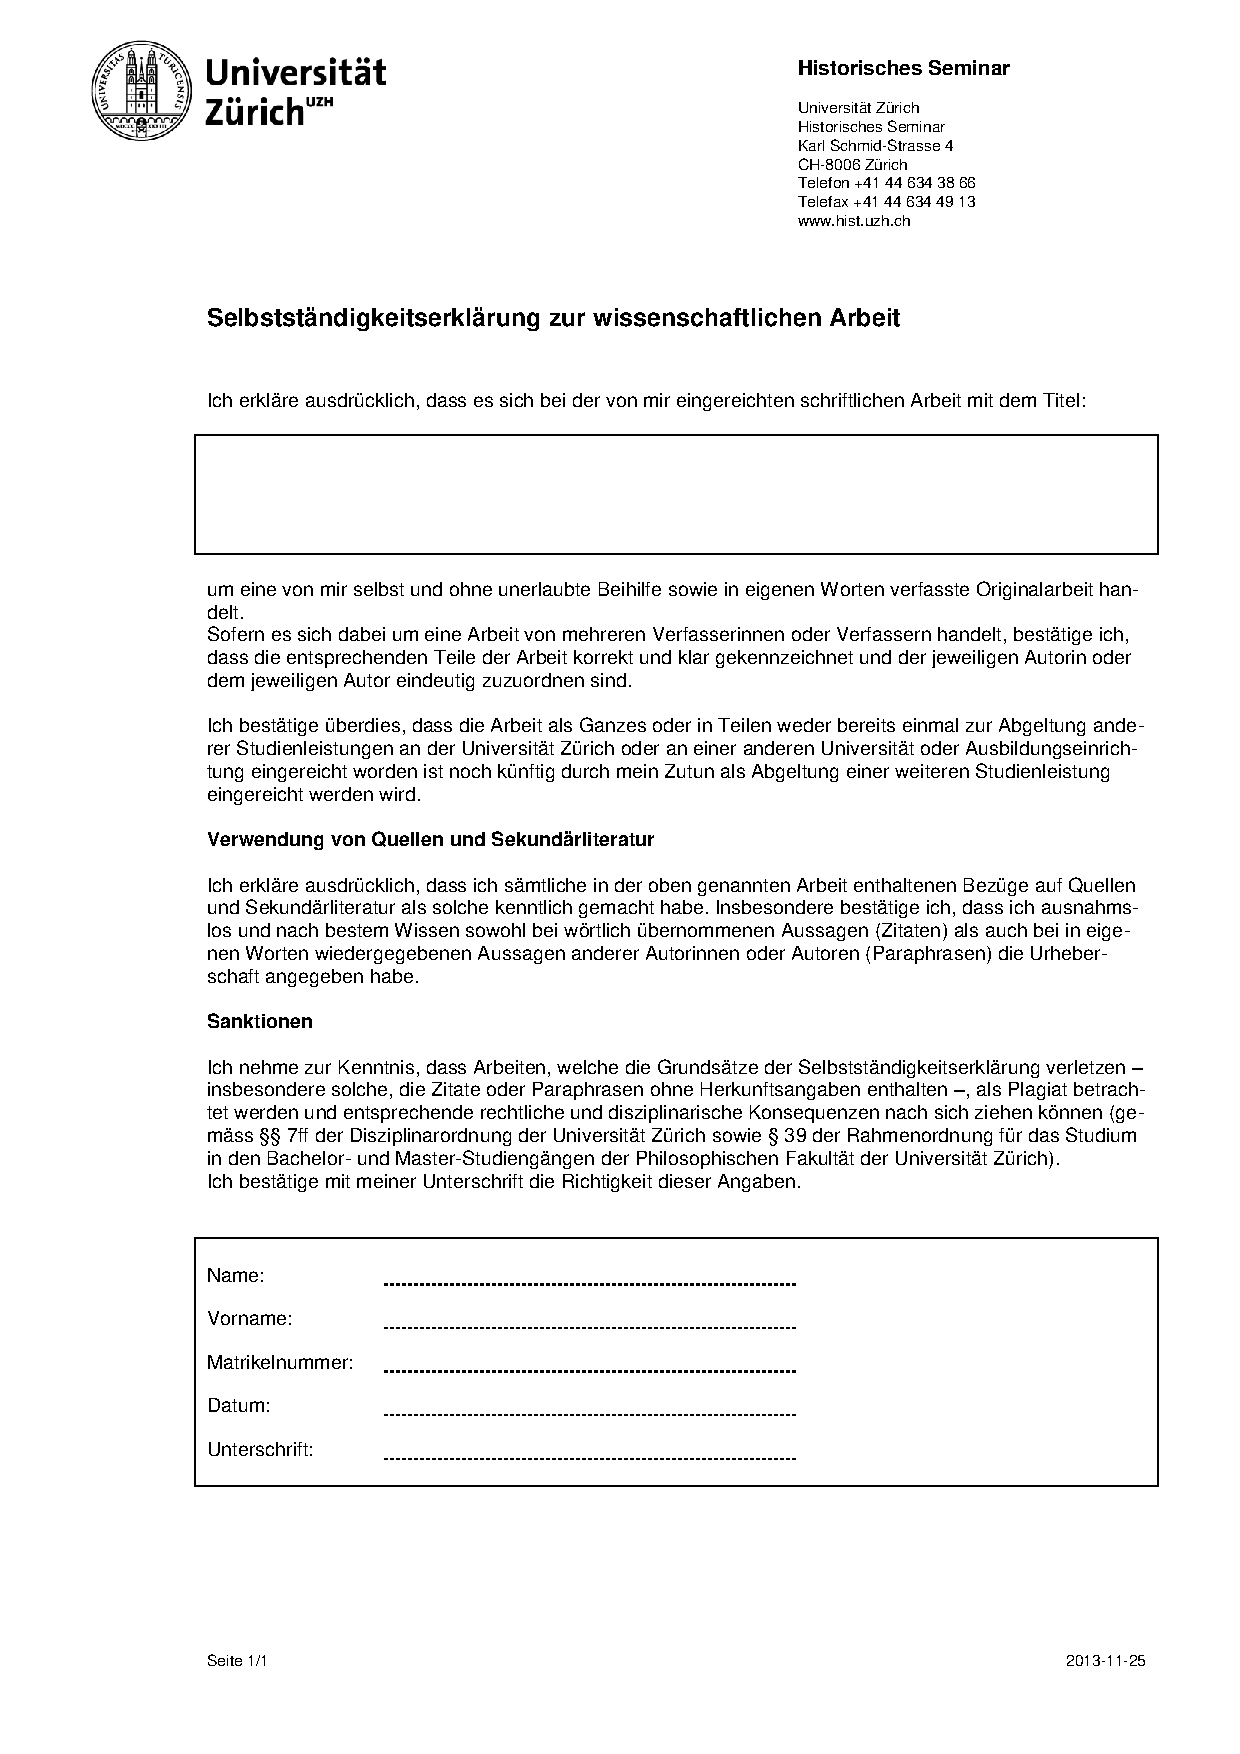
\includegraphics[width=\paperwidth,height=\paperheight,keepaspectratio]{./addendum/selbststaendigkeitserklaerung.pdf}
\end{document}
